\documentclass[11pt]{article}

\usepackage[margin=1in]{geometry}
\usepackage[T1]{fontenc}
\usepackage[utf8]{inputenc}
\usepackage{microtype}
\usepackage{amsmath,amssymb}
\usepackage{amsthm}
\usepackage{graphicx}
\usepackage{float}
\usepackage{array}
\usepackage{booktabs}
\usepackage{longtable}
\usepackage{tabularx}
\usepackage{xcolor}
\usepackage{tikz}
\usepackage[numbers,sort&compress]{natbib}
\usepackage[hyphens]{url}
\usepackage[colorlinks=true,linkcolor=blue!50!black,citecolor=blue!50!black,urlcolor=blue!50!black]{hyperref}

\usetikzlibrary{arrows.meta,positioning,fit,shapes.geometric}
\urlstyle{tt}
\emergencystretch=3em
\raggedbottom
\hbadness=10000
\floatstyle{ruled}
\newfloat{algorithm}{t}{loa}
\floatname{algorithm}{Algorithm}
\newtheorem{lemma}{Lemma}
\newtheorem{proposition}{Proposition}

\newcommand{\systemname}{AEN}
\newcommand{\athena}{Athena}
\newcommand{\aria}{Aria}
\newcommand{\artemis}{Artemis}
\newcommand{\rab}{RAB}
\newcommand{\artifact}[1]{\textit{evidence record}}
\newcommand{\status}[1]{\textsc{#1}}

\title{Artificial Evaluation Network (AEN): Runtime-at-Boot, Certified Context Loading, and Triadic Controller Algorithms for Mathematical Reasoning}
\author{
  Aaditya Paudel \\
  \small Research preprint
}
\date{April 2026}

\begin{document}
\maketitle

\begin{abstract}
Mathematical reasoning systems are often evaluated as if accuracy were determined only by model weights. The Artificial Evaluation Network (\systemname{}) studies a different scaling surface: long-context runtime memory, certified dataset loading, role-separated inference, and controller-managed finalization. The system loads role-specific boot memory into long-context sessions, verifies that each role can recall certified records through Runtime-at-Boot (\rab{}), and then runs a bounded triadic protocol in which \athena{} proposes and synthesizes, \aria{} pressure-tests proof structure, and \artemis{} audits computation and edge cases.

The core contribution is a deployable runtime architecture rather than a new model checkpoint. AEN combines Yet another Rotary Position Embedding extension (YaRN)-style long-context enablement, \rab{} certification, a three-body controller protocol, Canon v2.1 YAML-style problem distillation, strict closeout parsing, transcript export, and safe-memory dataset loading. These components make the solve process auditable: the paper separates memory loading from memory certification, role dialogue from controller state, mathematical confidence from final-answer emission, and external benchmark claims from internal diagnostics.

This paper presents the architecture as a reproducible systems method for constrained mathematical reasoning. It reports the implemented protocol, the dataset-loading and certification surfaces, diagnostic runs, and the remaining evaluation plan. The goal is not to claim that context memory alone proves mathematical competence, but to show how certified runtime memory and controller algorithms can make long-context model sessions inspectable under fixed offline deployment constraints.
\end{abstract}

\tableofcontents
\clearpage

\section{Introduction}

Large language models can solve difficult mathematical problems, but an exact-answer mathematical deployment is not only a language-model benchmark. It is a runtime system. A model or set of models must be loaded under fixed memory and wall-clock limits, receive the correct problem statement, preserve the evaluator's answer contract, avoid drift across long contexts, and emit a single normalized answer. A mathematically promising trace that selects the wrong transcription, loops on a false heuristic, or fails to normalize into the expected answer field is still invalid for evaluation.

The usual adaptation routes change model weights. Supervised fine-tuning and instruction tuning train on demonstration-style targets or instruction-formatted task collections, thereby teaching the model to imitate desired output behavior under a data distribution \citep{wei2021finetuned,ouyang2022training}. Reinforcement learning from human feedback (RLHF) trains a reward model from preference comparisons and then optimizes the policy against that reward model \citep{christiano2017deep,ouyang2022training}. These methods are powerful, but they are expensive axes for a constrained mathematical notebook: they require training compute, curated demonstrations or preference data, and, for reinforcement-learning-from-human-feedback-style pipelines, substantial human feedback infrastructure. They also remain output-shaping methods; after deployment, the system must still load the right context, verify the problem object, control dialogue, and emit an evaluator-valid answer.

This paper studies a different axis: inference-time curriculum and controller design. \rab{} treats the model as a reader before it becomes a solver. Role-specific boot datasets are loaded into long-context sessions; a simple certification test is then run at boot to check whether the model actually read and can recall the injected memory; only then does the solve loop begin. In human terms, this is like studying for a test before taking the test. It is not a replacement for all fine-tuning, but it is a lower-cost runtime mechanism for situations where changing weights is unavailable, too expensive, or too slow relative to the evaluation cycle.

\systemname{} combines this boot-time curriculum with a triadic controller algorithm. A single model instance can drift, repeat itself, over-trust a clean heuristic, or spend scarce tokens defending an early mistake. AEN is designed to improve practical accuracy over base-weight one-shot behavior through strict runtime discipline rather than through weight changes alone. Any naming convention could be used for role separation; this implementation adopts three generic AI role names. The \athena{}--\aria{}--\artemis{} protocol splits the pressures into roles: \athena{} preserves the problem object and later synthesizes, \aria{} attacks and repairs proof structure, and \artemis{} audits computation, edge cases, and candidate consistency. The AEN controller algorithm is the runtime procedure responsible for turn order, source-of-truth injection, transcript collection, confidence parsing, fallback labeling, and final answer emission.

The main advantage of \rab{} is that better curriculum data can improve inference behavior without retraining the model. The better the injected dataset, the better the model's test-time behavior can become, provided the memory teaches reusable mathematical procedures rather than answer leakage or surface-level templates. AEN therefore treats dataset loading, certification probes, safe-memory policy, and test-set separation as first-class components. The present implementation curates shorter, role-specific boot records for the three-role architecture and separates memory certification from solve-time scoring. This separation matters for any exact-answer evaluation because the target is mathematical performance, not recall of answer-bearing examples.

For \rab{}, a comprehensive boot dataset can consume a large prompt budget. More available context permits richer role memory, longer certification traces, and more complete peer transcripts. AEN therefore uses recent Qwen-family models with YaRN-style long-context enablement: each role session is configured for an approximately one-million-token context, and the three-role architecture distributes the effective context budget across roughly three million total tokens. Because this much context also demands efficient serving throughput, AEN uses the vLLM inference-serving library for model servers, with role sessions exposed as separate runtime endpoints. Together, Qwen-family long context, YaRN enablement, vLLM inference serving, role-specific boot datasets, and controller-visible budget accounting form the systems substrate for the AEN architecture summarized in Table~\ref{tab:contribution-roadmap}.

\section{Contribution Roadmap}

The paper is organized around system events rather than implementation version names. Table~\ref{tab:contribution-roadmap} gives the reader-facing map.

\begin{table}[p]
\centering
\scriptsize
\setlength{\tabcolsep}{4pt}
\renewcommand{\arraystretch}{1.08}
\begin{tabularx}{\textwidth}{@{}>{\raggedright\arraybackslash}p{0.20\linewidth}>{\raggedright\arraybackslash}p{0.36\linewidth}>{\raggedright\arraybackslash}X@{}}
\toprule
Event & What was achieved & Why it matters \\
\midrule
Dataset surfaces & AEN builds four dataset surfaces: three role-specific boot datasets loaded at runtime and one separate exact-answer test dataset. & Runtime memory, certification data, and evaluation rows are separated rather than treated as one undifferentiated prompt corpus. \\
YaRN long-context enablement & AEN treats multi-million-token-class context as a runtime substrate for role memory, problem transcripts, and controller state. & Long context becomes useful only when memory loading, certification, and truncation are measured rather than assumed. \\
vLLM inference-serving role endpoints & Role sessions are served through endpoints provided by the vLLM inference-serving library rather than a single undifferentiated model call. & Large-context multi-role inference becomes operationally feasible only when serving throughput, endpoint separation, and runtime health are part of the system. \\
\rab{} & Role memory is loaded from boot datasets and certified through deterministic probes before solve-time use. & The controller can distinguish a role that merely has a prompt from a role that demonstrated recall of its boot records. \\
Dataset loading and publication controls & Boot-study files, certification probes, safe-memory mode, and evaluation rows are treated as separate dataset objects. & This keeps role memory, certification state, and answer-bearing test data from being silently conflated. \\
3-body protocol & \athena{}, \aria{}, and \artemis{} receive distinct mathematical jobs: synthesis, proof-structure pressure, and computation/audit. & Same-family model instances are made more useful by role separation and turn discipline rather than by unconstrained debate. \\
Controller algorithm & The AEN controller algorithm manages prompt assembly, loop count, candidate parsing, confidence gates, fallback labeling, and final emission. & A final integer becomes a system decision with a recorded mode, not an accidental substring in model prose. \\
Canon v2.1 YAML schema & First-turn problem intake is structured into a YAML-style object ledger before route selection. & It attacks the most damaging failure class: semantic drift before the system has preserved the live mathematical object. \\
Diagnostics and reporting & Runs are separated into structural checks, internal diagnostics, attached tests, and external contest-style evaluations. & The paper can report progress without overstating what a local or memory-bearing run proves. \\
\bottomrule
\end{tabularx}
\caption{Reader-facing roadmap of the main AEN achievements covered in this paper.}
\label{tab:contribution-roadmap}
\end{table}

\section{Why Runtime Architecture Matters}

\subsection{Why inference-time architecture matters}

A common response to weak reasoning is to post-train the model: supervised fine-tuning on worked solutions, adapter methods such as Low-Rank Adaptation (LoRA), and preference or reinforcement learning from human feedback pipelines are all established ways to change model behavior \citep{hu2021lora,christiano2017deep,ouyang2022training}. These methods are primarily output-optimized: they train the model to imitate or prefer target completions, proof styles, answer formats, and conversational behaviors. At large scale, that route remains important. The claim of AEN is narrower: when the available dataset, compute budget, and evaluation cycle are limited, a substantial part of the reliability problem can be attacked from the input side instead. Runtime architecture optimizes what the fixed-weight model is made to read, remember, compare, and emit during the solve session.

The evidence around post-training supports this caution. FLAN-style instruction tuning shows that instruction-formatted mixtures can improve broad zero-shot behavior when scaled across model size, task mixture, and chain-of-thought data \citep{wei2021finetuned,chung2022scaling,longpre2023flan}. LIMA shows a complementary result: a 65B-parameter LLaMA model fine-tuned on 1,000 curated examples can learn strong response behavior, while the authors argue that most knowledge remains inherited from pretraining \citep{zhou2023lima}. These results make post-training valuable, but they also clarify what small post-training often buys first: imitation of a desired response surface. Mathematical reliability still depends on whether the model has the right problem, the right intermediate facts, the right checks, and the right finalization constraints active at inference time.

The mathematical fine-tuning literature sharpens the same point. \citet{yuan2023scalingmath} find that ordinary supervised fine-tuning (SFT) for mathematical reasoning scales with data amount, while rejection-sampling fine-tuning over correct reasoning paths substantially outperforms ordinary supervised fine-tuning in their Grade School Math 8K (GSM8K) setting. \citet{dong2024abilities} show that supervised-fine-tuning data composition creates different scaling patterns for math, code, and general alignment, with possible conflicts and forgetting. \citet{chen2025rethinking} show that, under pass@\(N\) test-time search, longer cross-entropy fine-tuning can decrease pass@\(N\) accuracy through overconfidence. A recent math/domain-shift study reports cases where instruction-tuned variants underperform base models in zero-shot chain-of-thought settings and degrade under perturbation \citep{munjal2026instructiontuned}. The supported claim is therefore not that post-training fails; it is that post-training is data- and protocol-sensitive, and small or mismatched post-training runs can optimize the wrong surface.

Runtime context is the complementary, input-optimized lever. GPT-3 few-shot evaluation shows that task demonstrations supplied purely through text interaction can change behavior without gradient updates \citep{brown2020fewshot}. Chain-of-thought prompting shows that a few in-context reasoning traces can improve arithmetic, commonsense, and symbolic reasoning, including strong gains on GSM8K with eight exemplars for a 540B model \citep{wei2022cot}. Least-to-most prompting further shows that decomposing a problem into subproblems inside the prompt can improve generalization to harder compositional and math reasoning tasks \citep{zhou2022leasttomost}. These results suggest a practical baseline: before changing weights, a strong base model can often be made more capable by changing the curriculum, examples, decomposition, and constraints it receives in context.

AEN turns that baseline into a runtime architecture. It treats session memory as a curriculum injected into context, then uses role separation and a controller algorithm to assign responsibility for problem preservation, proof construction, computation audit, synthesis, and final answer eligibility. This does not replace large-scale post-training. It asks a different systems question: how far can a fixed-weight model go when the inference environment is designed as carefully as the model output is usually trained? The rest of the paper answers that question by specifying the AEN runtime, its boot memory discipline, its triadic protocol, and its evidence trail.

\subsection{Limits of single-agent answer generation}

A single-agent solver has a simple interface: receive a problem, produce a solution, extract an answer. This simplicity is appealing, but it hides an important runtime limitation. During one continuous generation, earlier tokens are already fixed. The model can continue by writing a correction, but the runtime has not converted its partial answer into a fresh object for independent inspection. In long contexts, the situation becomes more fragile: relevant information can be harder to use reliably as context grows or as important material sits away from the prompt boundaries \citep{liu2024lostmiddle}. Intrinsic self-correction is also limited; without external feedback, LLM reasoning self-correction can fail to improve and can even degrade performance \citep{huang2023selfcorrect}. A single response therefore tends to mix route selection, derivation, checking, confidence, and final answer emission inside one stream.

The advantage of multi-agent runtime design is that it externalizes that stream. A chunk of model-generated reasoning can be captured by the controller algorithm and supplied as an input message to another role. The next role receives the previous output as something to inspect, challenge, repair, or route around, rather than as tokens it is currently committed to producing. Self-Refine shows the general value of turning an initial output into an object for feedback and refinement \citep{madaan2023selfrefine}. Multiagent debate shows the same idea with multiple model instances: agents propose and critique answers over rounds, improving factuality and mathematical or strategic reasoning relative to a single response \citep{du2023multiagentdebate}. CAMEL studies role-playing as a way to coordinate communicative agents with distinct responsibilities \citep{li2023camel}. AutoGen generalizes multi-agent conversation into a programmable framework for tasks including mathematics and coding \citep{wu2023autogen}. ChatDev applies specialized communicative agents to software development, where design, implementation, testing, and debugging are naturally separate responsibilities \citep{qian2023chatdev}.

AEN follows this literature but narrows the interface for exact-answer reasoning. The target is not open-ended debate or a generic agent chat. The target is a bounded, controller-visible sequence in which one model's answer attempt becomes another role's input object before finalization. Route diversity matters only if the controller algorithm can also record which role proposed the answer, which role checked it, what memory was visible, what finalization mode selected the value, and which evidence record supports the decision. A two-body solver-verifier protocol can be efficient, and earlier AEN development used that pattern as a useful baseline. The three-body protocol is more generalizable: it separates synthesis, proof-structure pressure, and computation/audit into distinct roles that can scale without forcing one verifier to carry every non-solver duty. This is why AEN uses a triad rather than a lone solver as its general protocol surface.

\section{From 2-Body Protocol to 3-Body Protocol}

AEN's triadic protocol grew out of a public two-model evaluator and a sequence of private runtime studies \citep{paudel2026twollm}. The important primitive was not merely that two models could be compared side by side. It was that a controller algorithm could turn one model's generated reasoning into a fresh input object for another model, preserve the speaker/listener boundary, record the transcript, and normalize the final integer separately from the prose that suggested it. This is the bridge from a one-body model call to a protocol: the runtime can decide which generated artifact becomes visible, which role receives it, and which answer is eligible for emission.

The first stage was a local two-body protocol on consumer hardware: Qwen-family 2-billion-parameter (2B) and 4-billion-parameter (4B) models running through a pure Transformers stack on an NVIDIA RTX 5060 Ti 16 GB graphics processing unit (GPU) machine. That stage was deliberately small. Its purpose was to establish the mechanics of solver/verifier separation under tight memory limits: separate prompts, addressed turns, normalized integer extraction, visible logs, and a reproducible way to compare a one-body response with a two-body response. The local smoke tests from this stage are not mathematical benchmark evidence, but they establish the basic controller surface on which later AEN runs depend.

The next stage moved the same two-body idea to a Linux runtime with NVIDIA H100 graphics processing unit (GPU) acceleration and Qwen-family 9-billion-parameter (9B) models, still before RAB memory injection. This stage tested whether protocol structure alone could change behavior when weights and problem context were otherwise fixed. The development notes record the key motivation: examples existed where a single 9B solve path failed, while a two-body solver-verifier path could recover because the verifier received the solver's attempt as an object to attack rather than as tokens it had already committed to generating. This became the first strong reason to treat role-separated inspection as a systems lever rather than only as repeated sampling.

A stricter historical version paired a Qwen3.5-9B solver with a Phi-4-reasoning-vision-15B verifier. The motivation was model diversity: two different model families, with different pretraining mixtures and inductive biases, should in principle have produced more novel synthesis than two copies of the same family. In practice, the mismatch was counterproductive. The Phi verifier was weaker than expected relative to the Qwen 9B solver in the non-thinking text setting, and collaboration was brittle: the roles sometimes refused to cooperate, and when they did cooperate, reasoning quality did not improve enough to justify the added complexity. This stage was still valuable because it clarified what the verifier contract needed to be. The verifier could not merely disagree or re-solve; it had to locate a concrete error, explain the failure, propose a minimal fix, and only then suggest an integer.

The next natural test was a same-family asymmetric pair: a Qwen-family 27-billion-parameter-class (27B-class) solver with a 4B verifier/clerk. This removed the cross-family collaboration failure and produced more coherent interaction, but it introduced a new bottleneck. The 27B model dominated the mathematical route, while the 4B model often behaved more like a summarizer and local self-correction assistant than an independent refuter. Invalid claims from the larger model were not attacked sharply enough. At the same time, the runtime was near the edge of the vLLM inference-serving resource envelope: key-value (KV)-cache headroom and graphics-processing-unit-utilization allocation became first-order constraints. The lesson was that scale asymmetry alone did not solve collaboration. It concentrated too many duties in the large model and left the smaller partner unable to contribute enough proof pressure.

\begin{table}[!htbp]
\centering
\scriptsize
\begin{tabularx}{\linewidth}{p{0.18\linewidth}p{0.24\linewidth}X}
\toprule
Stage & Runtime/model surface & What it contributed to AEN \\
\midrule
Local two-body & Qwen-family 2B/4B, pure Transformers, NVIDIA RTX 5060 Ti 16GB & Established solver/verifier prompting, addressed turns, transcript capture, and integer normalization under tight memory. \\
H100 9B/9B & Qwen-family 9B pair on Linux with NVIDIA H100 graphics-processing-unit acceleration, before boot-memory injection & Showed that role-separated inspection could change solve behavior without changing weights. \\
Qwen9B/Phi15B & Qwen3.5-9B solver with Phi-4-reasoning-vision-15B verifier & Tested cross-family diversity; exposed collaboration refusal and capability mismatch while sharpening the verifier-actionability contract. \\
Asymmetric large/small & Qwen-family 27B-class solver with 4B verifier/clerk & Improved coherence but showed 27B route dominance, weak 4B refutation, and vLLM inference-serving/key-value-cache pressure near the graphics-processing-unit budget. \\
AEN triad & Three same-family Qwen3.5-9B roles under a controller algorithm & Fits the one-H100 envelope while separating synthesis, alternate proof structure, computation audit, and final answer eligibility. \\
\bottomrule
\end{tabularx}
\caption{Protocol lineage from the two-body solver-verifier baseline to the three-body AEN protocol. The table describes development stages and mechanism, not a standalone benchmark leaderboard.}
\label{tab:two-body-lineage}
\end{table}

The three-body AEN protocol responds to those failures. Cross-family pairing was brittle, and large/small two-body pairing overloaded the larger model. AEN therefore returns to same-family Qwen3.5-9B roles, where parsing, prompting conventions, confidence syntax, and convergence behavior are easier to align. Qwen-family context windows can also be extended through YaRN-style enablement; after repeated runtime trials, all three models could be served in one local run with roughly one million tokens of context per role. The result is a three-session system with approximately three million total distributed context tokens.

The transition from two bodies to three was therefore not a cosmetic role split. The two-body protocol was useful as a solver-verifier baseline, but it left one side overloaded whenever the route itself, the arithmetic audit, and the final-answer decision all needed separate pressure. The third role gives the controller algorithm a cleaner runtime graph: one role can preserve and synthesize the main route, one can construct or attack proof structure, and one can focus on computation and edge cases. That extra body also makes later scaling more natural, because additional roles can be added as new pressure points rather than as vague extra debaters.

The deeper reason for moving from two bodies to three was to build a local agent swarm rather than a single solver-verifier pair. The triad is the smallest AEN form that separates synthesis, alternate route construction, computation audit, memory certification, and finalization while still fitting on one H100-class runtime. In principle, the same controller-algorithm pattern can scale beyond three roles to an \(n\)-model swarm, with final-answer eligibility remaining a controller-algorithm decision. Figure~\ref{fig:aen-three-body-protocol} summarizes this protocol boundary.

\begin{figure}[H]
\centering
\makebox[\textwidth][c]{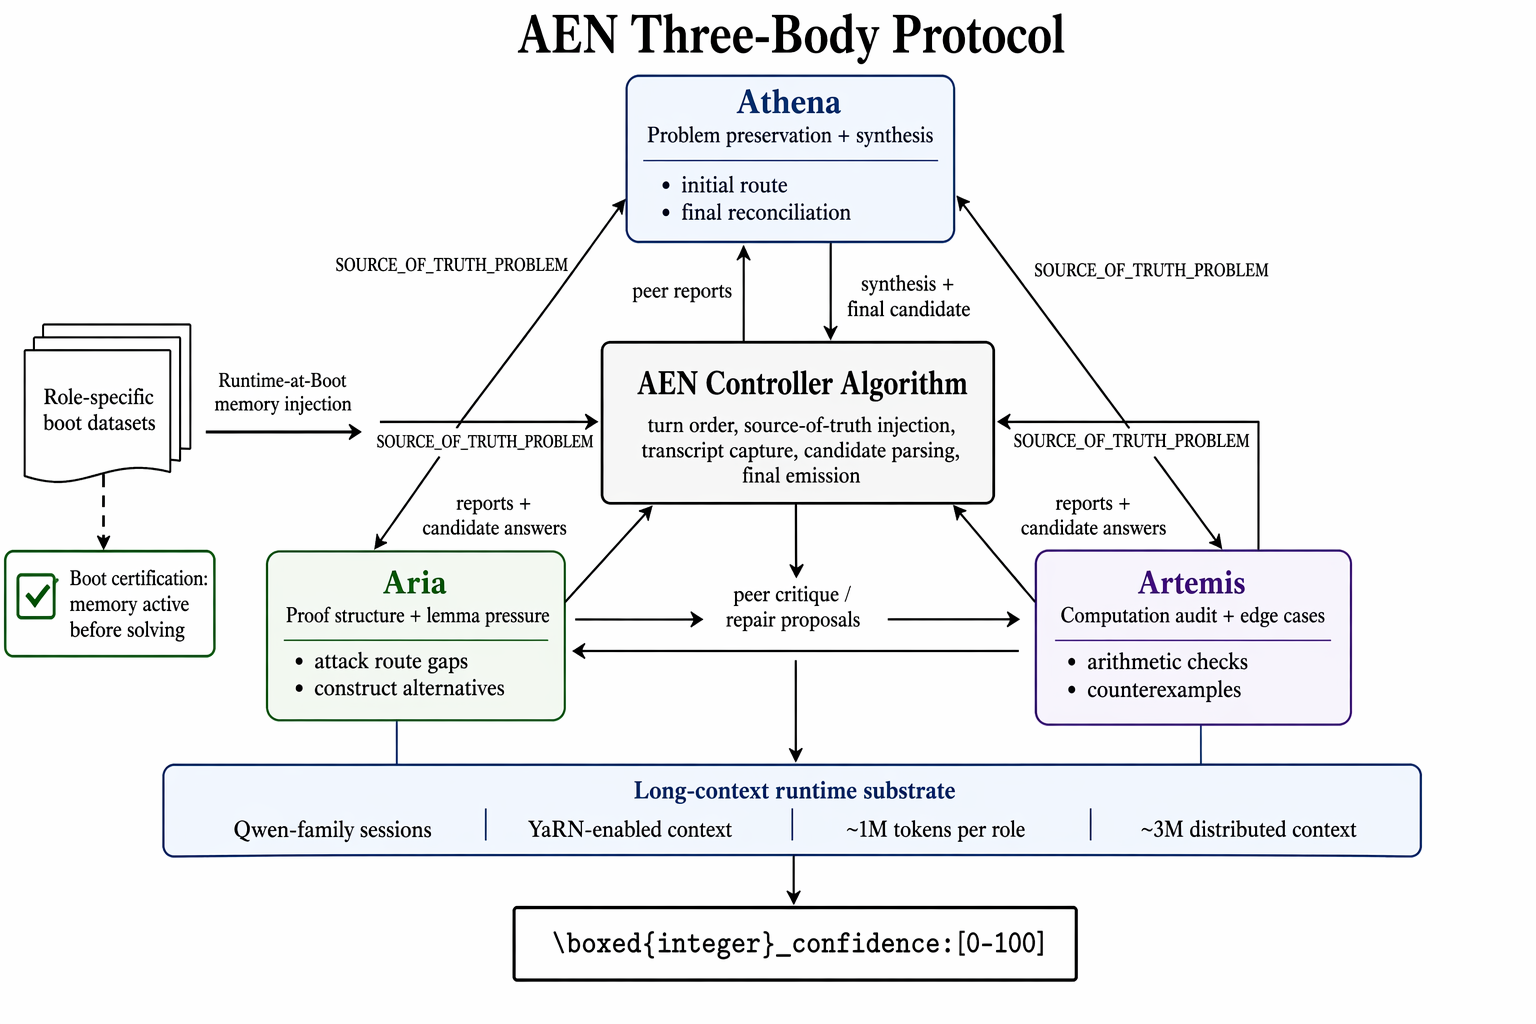
\includegraphics[width=1.14\textwidth]{diagrams/aen_three_body_protocol.png}}
\caption{AEN three-body protocol schema. Three independently served Qwen-family role sessions operate over a long-context runtime substrate, while the AEN controller algorithm manages source-of-truth injection, report flow, candidate parsing, and final answer emission.}
\label{fig:aen-three-body-protocol}
\end{figure}

Theoretically, this architecture can extend to a hierarchical \(n\)-body local swarm: each node runs the AEN three-body protocol, while parent-child links route subproblems, summaries, and reports. The experiments in this paper do not validate the proposed \(n>3\) swarm; they only establish the implemented three-role runtime boundary. Figure~\ref{fig:aen-n-body-local-protocol} shows the proposed scaling picture.

\begin{figure}[p]
\centering
\makebox[\textwidth][c]{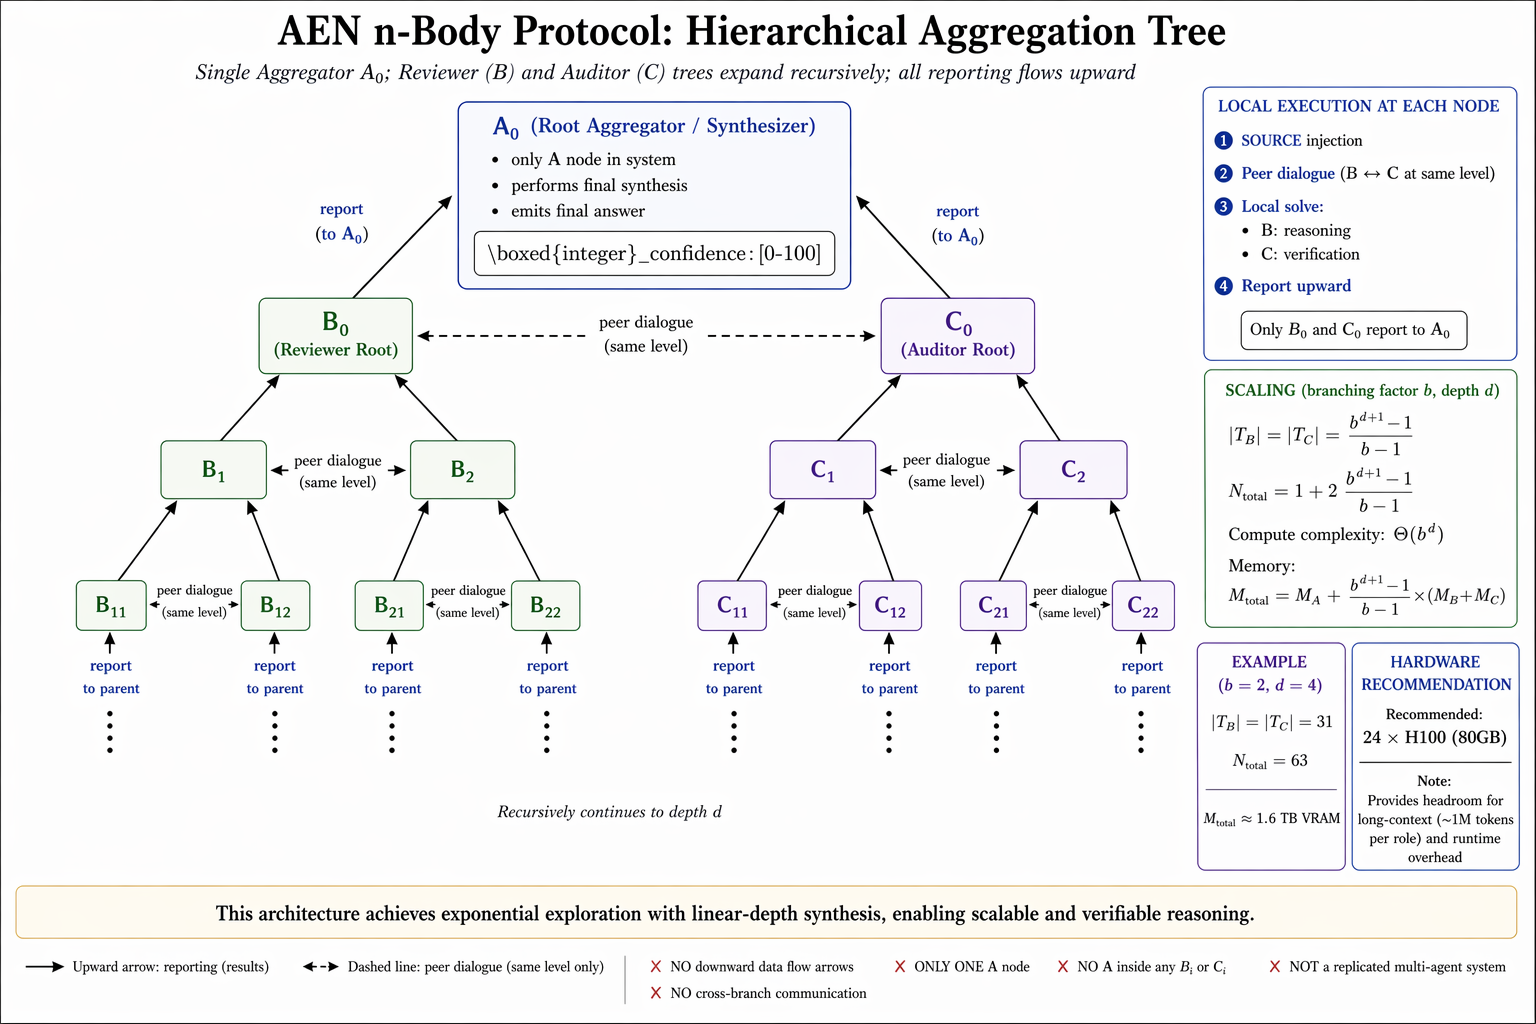
\includegraphics[width=1.04\textwidth]{diagrams/aen_n_body_local_protocol.png}}
\caption{Proposed AEN \(n\)-body local swarm extension. Each node runs the AEN three-body protocol independently; parent-child communication, report aggregation, and root synthesis define a theoretical hierarchical scaling route. This figure is a design proposal, not an experimentally validated \(n>3\) result in this paper.}
\label{fig:aen-n-body-local-protocol}
\end{figure}

\clearpage

\section{System Overview: Runtime Memory plus Controller}

The AEN runtime begins before any contest problem is solved. The first architectural event is \rab{}: role-specific boot records are loaded into long-context model sessions, and the controller algorithm runs certification probes to check whether each role can recall the injected memory. A role that merely has a prompt is not yet treated as an active solver. It becomes eligible only after the runtime demonstrates that the relevant memory is live in the session. This is the difference between storing a curriculum somewhere on disk and making that curriculum operational inside the inference context.

The deployed AEN instance uses three same-family Qwen3.5-9B-class role sessions rather than a single monolithic model call. The public Qwen-family long-context literature is relevant because Qwen-family decoder models use Rotary Position Embedding (RoPE)-style positional structure, and the Qwen2.5-1M release documents a transformer architecture with RoPE, Swish-Gated Linear Unit (SwiGLU), Root Mean Square Layer Normalization (RMSNorm), grouped-query attention, query-key-value (QKV) bias, and a context length of about one million tokens under its long-context serving stack \citep{yang2025qwen25oneM,qwen2025qwen25oneMcard}. AEN uses that design direction as a runtime substrate: each role receives its own long-context session, and the controller algorithm distributes memory and transcript state across the three sessions instead of forcing all state into one prompt.

Once boot eligibility is established, the controller algorithm assembles the solve-time prompt surface. It injects the source-of-truth problem statement, selects which memory blocks and peer records are visible, enforces the turn schedule, records transcript artifacts, parses candidate answers and confidence values, and emits the final evaluator-facing answer. The controller algorithm is therefore not just a message router. It is the runtime boundary between model prose and the submitted artifact.

AEN uses three role sessions because the pressures of exact-answer mathematical solving fail in different ways. The same generation should not simultaneously preserve the problem object, invent the route, audit arithmetic, judge confidence, and decide the wrapper answer. The three-role design gives each pressure a named runtime location:

\begin{itemize}
  \item \textbf{\athena{}} is the primary mathematical solver and synthesizer. It proposes routes, carries the main derivation, and produces controller-facing mathematical claims.
  \item \textbf{\aria{}} is the proof-structure and alternate-derivation role. It is intended to provide route diversity, restate proof obligations, and identify structural gaps from a different angle.
  \item \textbf{\artemis{}} is the computation, audit, and verifier role. It checks arithmetic, validates candidate answers, and records whether the final route is sufficiently supported.
\end{itemize}

Final-answer selection is taken from the parsed role candidates rather than from a loose prose phrase. If all three models agree on the same integer, the controller algorithm emits that consensus answer. If two models agree and one disagrees, the controller algorithm emits the majority answer. If no two parsed answers match, the controller algorithm emits the candidate with the highest parsed confidence, while recording the fallback mode. In an integer-answer notebook setting, the final value must be a single normalized integer in the evaluator wrapper. For that reason, controller finalization is part of the mathematical system rather than a formatting afterthought.

The architecture differs from a generic multi-agent transcript in two ways. First, AEN emphasizes artifact responsibility: every important transition should be visible in logs, manifests, transcripts, prompt payloads, or result files. Second, AEN treats finalization as a controller-algorithm function rather than a final model flourish. This reduces the chance that a plausible answer phrase becomes the emitted answer without an explicit controller decision.

\begin{figure}[H]
\centering
\vspace{0.3em}
\makebox[\textwidth][c]{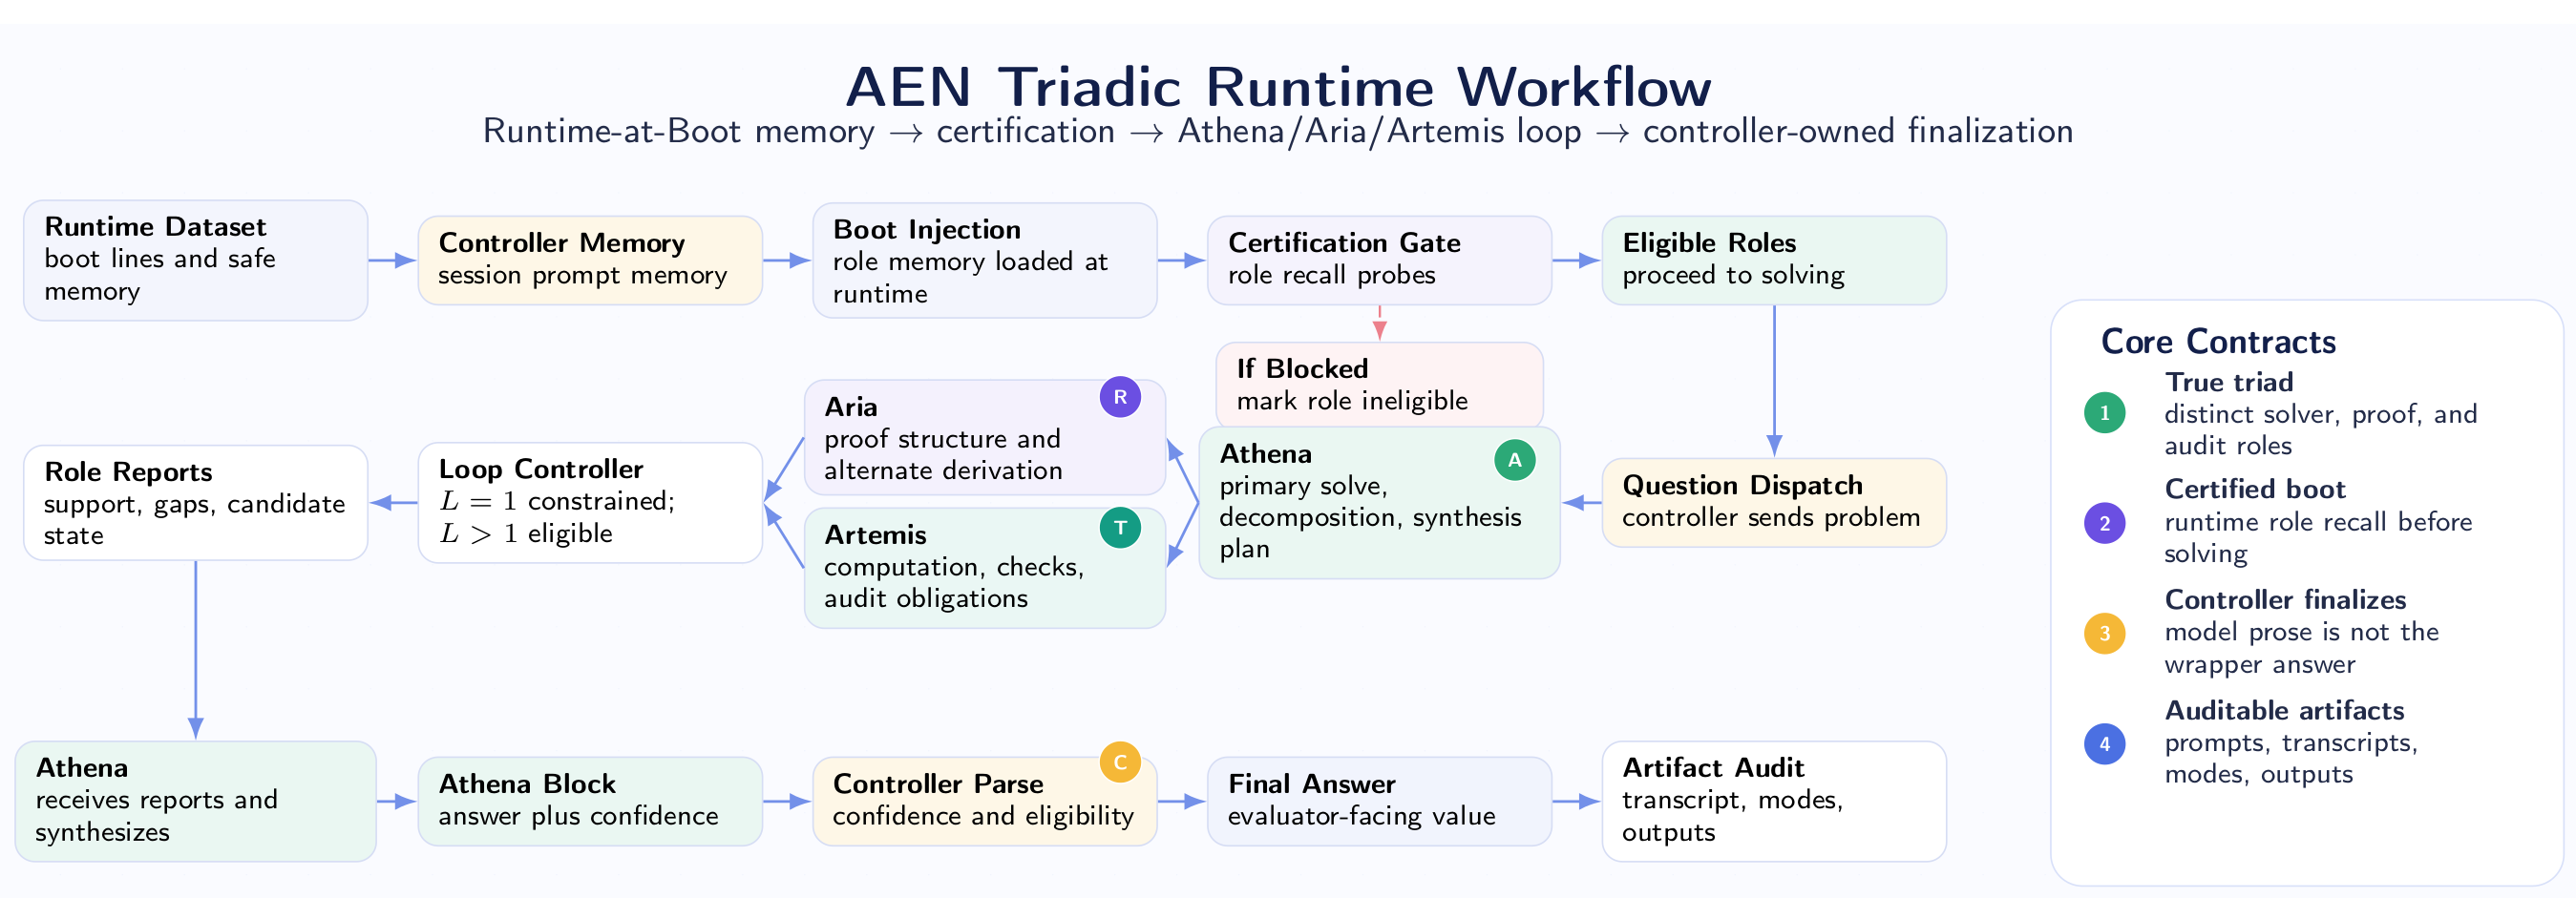
\includegraphics[width=1.25\textwidth]{diagrams/aen_architecture.png}}
\caption{AEN triadic runtime workflow. \rab{} certifies role eligibility before solve-time interaction; the AEN controller algorithm then manages prompt construction, transcript collection, report flow, candidate parsing, and final answer emission.}
\label{fig:architecture}
\label{fig:triadic-turn-protocol}
\end{figure}

\begin{table}[H]
\centering
\small
\renewcommand{\arraystretch}{1.16}
\begin{tabularx}{\linewidth}{p{0.18\linewidth}X X}
\toprule
Phase & Controller action & Evidence expected \\
\midrule
Preflight & Load packages, model endpoints, datasets, and notebook configuration. & Kernel metadata, bootstrap logs, runtime paths. \\
Certification & Run \rab{} probes and block roles whose memory is not certified. & RAB summary and per-role rows. \\
Solving & Schedule bounded role turns with safe memory and visible context. & Prompt payloads, transcripts, token and timing logs. \\
Audit & Parse candidate answers, confidence, and verification state. & Controller records, verification status, finalization mode. \\
Emission & Write the evaluator-facing integer and supporting artifacts. & Submission file, result log, transcript directory. \\
\bottomrule
\end{tabularx}
\caption{Operational phases of the AEN controller.}
\label{tab:phases}
\end{table}

\clearpage

\section{YaRN Long-Context Enablement}

The first enabling event is the long-context substrate. AEN is built around the idea that a model session can carry more than the immediate problem statement: it can carry role identity, method records, certified memory, prior controller state, peer reports, and problem-specific scratch structure. In practice, this only becomes useful when context length is paired with discipline. A multi-million-token context window can help preserve memory, but it can also hide stale assumptions, leak irrelevant records, or make the model drift semantically before it solves.

\subsection{Rotary Position Embedding (RoPE) as the positional substrate}

YaRN is best understood as a Rotary Position Embedding (RoPE)-scaling method, so the starting point is the Rotary Position Embedding mechanism itself. Rotary Position Embedding divides the query and key hidden dimensions into two-dimensional pairs. For a token at position \(m\), each pair is multiplied by the \emph{RoPE pair-rotation} matrix \citep{su2021roformer}
\begin{equation}
\label{eq:rope-pair-rotation}
R_{\theta_j}(m)=
\begin{pmatrix}
\cos(m\theta_j) & -\sin(m\theta_j)\\
\sin(m\theta_j) & \cos(m\theta_j)
\end{pmatrix},
\end{equation}
where \(\theta_j\) is the frequency assigned to that pair. Equation~\eqref{eq:rope-pair-rotation} is orthogonal, so it preserves vector norms. If \(u_m\) and \(v_n\) denote the unrotated query and key pair components at positions \(m\) and \(n\), then
\begin{equation}
\label{eq:rope-relative-kernel}
\bigl(R_{\theta_j}(m)u_m\bigr)^{\top}\bigl(R_{\theta_j}(n)v_n\bigr)
=u_m^{\top}R_{\theta_j}(n-m)v_n,
\end{equation}
because \(R_{\theta_j}(m)^{\top}R_{\theta_j}(n)=R_{\theta_j}(n-m)\). This is the key Rotary Position Embedding property: absolute positions are encoded through rotation, but the attention score naturally carries relative-position information \citep{su2021roformer}. The RoFormer paper also emphasizes that the rotation is norm-preserving and gives Rotary Position Embedding a useful long-distance decay behavior \citep{su2021roformer}.

The frequency \(\theta_j\) corresponds to the wavelength
\begin{equation}
\label{eq:rope-wavelength}
\lambda_j=\frac{2\pi}{\theta_j}.
\end{equation}
High-frequency dimensions have short wavelengths and are important for distinguishing nearby tokens; low-frequency dimensions have long wavelengths and support coarser long-range position information. This wavelength view is central to YaRN because stretching all dimensions equally can damage the local positional distinctions that the model learned during pretraining \citep{peng2023yarn}.

\subsection{YaRN scaling}
\label{subsec:yarn-scaling}

AEN relies on long-context Qwen-family sessions to keep role memory, certification probes, current problem state, peer transcripts, and controller state simultaneously available in-session. Yet another Rotary Position Embedding Extension (YaRN)-style scaling is used here as an enabling mechanism for that long-context runtime-memory substrate, not as a standalone theorem of improved reasoning quality \citep{peng2023yarn,yang2025qwen25oneM}.

For an attention head of even dimension \(d_h=2J\), decompose each query/key vector into \(J\) two-dimensional blocks. For a scalar angle \(\phi\in\mathbb R\), define
\begin{equation}
\mathbf Q(\phi)
:=
\begin{bmatrix}
\cos \phi & -\sin \phi\\
\sin \phi & \cos \phi
\end{bmatrix}.
\label{eq:yarn-Q}
\end{equation}
For Rotary Position Embedding frequency \(\theta_j\) and token position \(m\in\mathbb Z\), the \(j\)-th pair rotation is
\begin{equation}
\mathbf R_{\theta_j}(m):=\mathbf Q(m\theta_j),
\qquad j=1,\dots,J,
\label{eq:yarn-pair-rotation}
\end{equation}
and the full operator is
\begin{equation}
\mathcal R_{\boldsymbol\theta}(m)
:=
\operatorname{diag}\!\bigl(
\mathbf R_{\theta_1}(m),\dots,\mathbf R_{\theta_J}(m)
\bigr).
\label{eq:yarn-full-rope}
\end{equation}

Let \(L\) denote the pretrained context length, let \(L'=sL\) be the target extended context length with scale factor \(s>1\), and let
\begin{equation}
\lambda_j := \frac{2\pi}{\theta_j},
\qquad
r_j := \frac{L}{\lambda_j} = \frac{L\theta_j}{2\pi}.
\label{eq:yarn-wavelength-ratio}
\end{equation}
Following the Neural Tangent Kernel (NTK)-by-parts interpolation used in YaRN \citep{peng2023yarn}, define
\begin{equation}
\gamma(r)
:=
\begin{cases}
0, & r<\alpha,\\[3pt]
1, & r>\beta,\\[3pt]
\dfrac{r-\alpha}{\beta-\alpha}, & \alpha \le r \le \beta,
\end{cases}
\qquad \alpha<\beta,
\label{eq:yarn-ramp}
\end{equation}
and the frequency map
\begin{equation}
\theta'_j
:=
h_s(\theta_j)
:=
\bigl(1-\gamma(r_j)\bigr)\frac{\theta_j}{s}
+
\gamma(r_j)\theta_j.
\label{eq:yarn-frequency-map}
\end{equation}
Set \(\boldsymbol\theta'=(\theta'_1,\dots,\theta'_J)\) and define
\begin{equation}
\mathcal R_s(m)
:=
\mathcal R_{\boldsymbol\theta'}(m)
=
\operatorname{diag}\!\bigl(
\mathbf R_{\theta'_1}(m),\dots,\mathbf R_{\theta'_J}(m)
\bigr).
\label{eq:yarn-scaled-operator}
\end{equation}
Equivalently, YaRN acts blockwise as
\begin{equation}
T_s:\mathbf R_{\theta_j}(m)\longmapsto \mathbf R_{\theta'_j}(m).
\label{eq:yarn-block-transform}
\end{equation}

\begin{lemma}[Algebra of planar rotations]
\label{lem:yarn-rotation-identities}
For all \(\phi,\psi\in\mathbb R\),
\begin{align}
\mathbf Q(\phi)^\top &= \mathbf Q(-\phi), \label{eq:yarn-transpose}\\
\mathbf Q(\phi)\mathbf Q(\psi) &= \mathbf Q(\phi+\psi), \label{eq:yarn-composition}\\
\mathbf Q(\phi)^\top \mathbf Q(\psi) &= \mathbf Q(\psi-\phi). \label{eq:yarn-relative}
\end{align}
Therefore \(\mathbf Q(\phi)^\top\mathbf Q(\phi)=\mathbf I_2\), \(\det\mathbf Q(\phi)=1\), and \(\mathbf Q(\phi)\in \mathrm{SO}(2)\).
\end{lemma}

\begin{proof}
The transpose identity follows directly from Equation~\eqref{eq:yarn-Q}. Direct multiplication and the trigonometric addition identities give \(\mathbf Q(\phi)\mathbf Q(\psi)=\mathbf Q(\phi+\psi)\). Combining these two identities gives \(\mathbf Q(\phi)^\top\mathbf Q(\psi)=\mathbf Q(-\phi)\mathbf Q(\psi)=\mathbf Q(\psi-\phi)\). Setting \(\psi=\phi\) gives orthogonality. Finally, \(\det \mathbf Q(\phi)=\cos^2\phi+\sin^2\phi=1\).
\end{proof}

\begin{proposition}[Operator properties of YaRN-scaled RoPE]
\label{prop:yarn-operator}
Let \(q=(q_1^\top,\dots,q_J^\top)^\top\) and \(k=(k_1^\top,\dots,k_J^\top)^\top\in\mathbb R^{d_h}\), where \(q_j,k_j\in\mathbb R^2\). Then, for every \(m,n\in\mathbb Z\):
\begin{enumerate}
    \item \(\mathcal R_s(m)^\top \mathcal R_s(m)=\mathbf I_{d_h}\). Consequently, \(\|\mathcal R_s(m)x\|_2=\|x\|_2\) for all \(x\in\mathbb R^{d_h}\), and \(\|\mathcal R_s(m)\|_{2\to 2}=1\).
    \item \(\mathcal R_s(m)^\top \mathcal R_s(n)=\mathcal R_s(n-m)\). Consequently,
    \begin{equation}
    \left\langle \mathcal R_s(m)q,\mathcal R_s(n)k\right\rangle
    =
    \sum_{j=1}^{J} q_j^\top \mathbf Q\!\bigl((n-m)\theta'_j\bigr)k_j.
    \label{eq:yarn-blockwise-relative}
    \end{equation}
    \item If \(r_j\ge \beta\), then \(\theta'_j=\theta_j\), so \(\mathbf R_{\theta'_j}(m)=\mathbf R_{\theta_j}(m)\) for all \(m\in\mathbb Z\).
    \item If \(r_j\le \alpha\), then \(\theta'_j=\theta_j/s\), \(\lambda'_j=2\pi/\theta'_j=s\lambda_j\), and
    \begin{equation}
    \frac{L'}{\lambda'_j}=\frac{L}{\lambda_j},
    \qquad
    L'\theta'_j=L\theta_j.
    \label{eq:yarn-phase-preservation}
    \end{equation}
\end{enumerate}
\end{proposition}

\begin{proof}
Because \(\mathcal R_s(m)\) is block diagonal with blocks \(\mathbf Q(m\theta'_j)\), Lemma~\ref{lem:yarn-rotation-identities} applies to each block. Orthogonality of every block gives \(\mathcal R_s(m)^\top \mathcal R_s(m)=\mathbf I_{d_h}\), and therefore \(\|\mathcal R_s(m)x\|_2=\|x\|_2\) and \(\|\mathcal R_s(m)\|_{2\to2}=1\).

For the relative-position identity,
\[
\mathcal R_s(m)^\top\mathcal R_s(n)
=
\operatorname{diag}\!\bigl(
\mathbf Q(m\theta'_1)^\top\mathbf Q(n\theta'_1),
\dots,
\mathbf Q(m\theta'_J)^\top\mathbf Q(n\theta'_J)
\bigr)
=
\mathcal R_s(n-m).
\]
Substituting this into the dot product gives Equation~\eqref{eq:yarn-blockwise-relative}.

If \(r_j\ge\beta\), then \(\gamma(r_j)=1\), so Equation~\eqref{eq:yarn-frequency-map} gives \(\theta'_j=\theta_j\). If \(r_j\le\alpha\), then \(\gamma(r_j)=0\), so \(\theta'_j=\theta_j/s\). Hence \(\lambda'_j=2\pi/(\theta_j/s)=s\lambda_j\). Since \(L'=sL\), the endpoint phase budget is preserved:
\[
\frac{L'}{\lambda'_j}=\frac{sL}{s\lambda_j}=\frac{L}{\lambda_j},
\qquad
L'\theta'_j=sL\frac{\theta_j}{s}=L\theta_j.
\]
\end{proof}

\paragraph{Spectral cross-check.}
For each pair \(j\), the complexified matrix \(\mathbf Q(m\theta'_j)\) has eigenvectors \(e_\pm=(1,\mp i)^\top\) with eigenvalues \(e^{\pm i m\theta'_j}\). Since \(|e^{\pm i m\theta'_j}|=1\), the spectral radius is \(1\). Because \(\mathbf Q(m\theta'_j)\) is real orthogonal, its singular values are also \(1\). This independently confirms the isometric and non-expansive conclusion of Proposition~\ref{prop:yarn-operator}; it does not extend that conclusion to a theorem about downstream task accuracy.

Proposition~\ref{prop:yarn-operator} is intentionally operator-level. It establishes that YaRN-scaled Rotary Position Embedding remains orthogonal, preserves Rotary Position Embedding's relative-offset kernel structure, leaves the high-frequency endpoint unchanged, and preserves the pretrained phase budget at the low-frequency endpoint over the extended window. Performance statements beyond this proposition are empirical. YaRN reports compute-efficient context-window extension with substantially less long-context adaptation than prior approaches in its evaluations, including passkey retrieval at \(128\text{k}\) in evaluated checkpoints \citep{peng2023yarn}. Qwen2.5-1M further combines long-context model training with an inference framework including length extrapolation, sparse attention, chunked prefill, and serving-level optimizations \citep{yang2025qwen25oneM}. The public Qwen2.5-7B-Instruct-1M model card additionally warns that accuracy may degrade beyond \(262{,}144\) tokens without the specialized long-context framework \citep{qwen2025qwen25oneMcard}.

\paragraph{Hypothesis for AEN.}
Within AEN, the relevant claim is systems-level: if the controller injects relevant curriculum, certification traces, current problem state, and peer critiques while keeping those memories active, safe, and visible, then expanded context should improve runtime reasoning by increasing the amount of useful information that remains simultaneously accessible across the three role sessions before context exhaustion. This is a hypothesis about the full runtime architecture to be evaluated experimentally; it is not a direct corollary of Proposition~\ref{prop:yarn-operator}.

\section{Runtime-at-Boot (RAB): Certified Dataset Loading}

\rab{} is an inference-time curriculum and eligibility layer. Before a problem is dispatched, the controller algorithm injects role-specific study records into the active long-context session and asks whether the role can recover the relevant boot memory under controlled probes. Task-relevant method memory is therefore visible, auditable, removable, and testable inside the same session that will later solve. If a role cannot recover its boot memory, the controller treats that role as not boot-certified for the solve.

This design uses a different adaptation surface from supervised fine-tuning, instruction tuning, or reinforcement learning from human feedback. Those methods change the model's conditional distribution through parameter updates or reward optimization \citep{wei2021finetuned,christiano2017deep,ouyang2022training}. \rab{} changes the information environment at inference time. The distinction matters under small curated datasets and fixed notebook deployments: a boot record can be inspected, updated, excluded, certified, or labeled as answer-bearing without rebuilding a checkpoint. Weight updates can be powerful at scale, but they are harder to audit at the level of a single role instruction, proof obligation, or final-answer contract.

The empirical literature gives a reason to take session memory seriously. Few-shot prompting shows that a pretrained model can adapt behavior from examples supplied in the input without gradient updates \citep{brown2020fewshot}. Chain-of-thought prompting shows that in-context reasoning traces can improve arithmetic, commonsense, and symbolic reasoning, with the original study reporting that eight worked reasoning exemplars for a 540B model surpassed a fine-tuned GPT-3-with-verifier baseline on Grade School Math 8K \citep{wei2022cot}. Least-to-most prompting shows that decompositions supplied in context can improve generalization to harder compositional tasks \citep{zhou2022leasttomost}. A controlled comparison of in-context learning and fine-tuning further reports that, in data-matched settings, in-context learning can generalize more flexibly than fine-tuning on systematic holdouts, while also noting that fine-tuning can be improved with additional augmented data \citep{lampinen2025generalization}. These results do not imply that prompt memory dominates post-training universally. They support the narrower systems premise used here: when a strong base model is already deployed, high-quality in-session memory can be a competitive and more controllable adaptation path.

The second motivation is stochastic runtime behavior. Autoregressive language models define a distribution over continuations, and many reasoning evaluations explicitly exploit the fact that different samples from the same model can succeed or fail on the same prompt. The pass@\(k\) methodology used in code-generation evaluation measures the chance that at least one of \(k\) sampled completions is correct, and Codex-style results show large gains from repeated sampling \citep{chen2021codex}. Self-consistency applies the same inference-time idea to reasoning: sample multiple reasoning paths and select the most consistent answer, improving arithmetic and commonsense benchmarks over greedy chain-of-thought decoding \citep{wang2022selfconsistency}. In AEN, \rab{} is a boot-time sharpness screen, i.e., before expensive solve-time inference begins, the controller checks whether the current role session can recover the minimum role memory needed for disciplined work.

For AEN, the relevant advantage is therefore not pass@\(1\) on a fresh unconditioned model call. The relevant comparison is between a fixed-weight role that enters a solve cold and a fixed-weight role that enters with certified, role-specific memory already active in context. \rab{} turns that difference into a measurable precondition. The controller can ask whether Athena recalls synthesis discipline, whether Aria recalls proof-pressure obligations, whether Artemis recalls audit duties, and whether each role understands the final-answer contract before a live problem consumes solve-time tokens. The current gate is deliberately light: each certified line may receive up to three attempts, so a popular \texttt{Run All} competition or notebook session is not made brittle by a single harmless miss. This three-attempt schema mitigates bad boot states while allowing viable, sharper role sessions to proceed; it is an eligibility check, not a claim that the role has become mathematically optimal. This motivates dataset curation: boot memory must be compact, role-specific, reusable across problems, and separated from answer-bearing evaluation rows unless the run is explicitly labeled as a memory-recall experiment.

\subsection{RAB Working Schema}



The \rab{} working schema is executed by AEN's controller algorithm. At boot, the controller resolves a role-memory carrier for each active role and converts it into a role curriculum. A study row provides the text that may enter the role's prompt. A certification row provides a deterministic probe, usually a multiple-choice question with an expected answer. The controller joins certification probes to study rows by parent identifier, applies role-specific line limits and probe limits, and keeps only rows whose probes are ready. These limits are runtime knobs; the body of this section describes the mechanism, while observed line counts and elapsed times belong to the results section.

Prompt injection is explicit. The controller starts from the role identity prompt, selects bounded study lines with optional line and character caps, and appends them under a literal \texttt{FACTUAL\_MEMORY} header. The resulting prompt is written back into the role session prompt variables before solving. A separate validation pass confirms that the intended boot memory has actually loaded.

Certification is then run as an interaction, not as a file check. For each selected line, the controller builds a short gate prompt: the role is shown the study record, a question, and answer options, and is instructed to reply with exactly one capital letter. The response is normalized and compared against accepted answer variants. A correct answer advances to the next probe or certifies the line. An incorrect answer retries until the configured maximum attempts per line is exhausted; the default working schema allows up to three attempts. If a line fails after those attempts, the role is marked not boot-certified for that run.

After a role passes the gate, the controller can record a compact certification summary for downstream audit. The claim is not that the role has learned new weights or solved the benchmark; the claim is that the loaded session recovered selected role memory under a bounded certification procedure.

\begin{figure}[H]
\centering
\makebox[\textwidth][c]{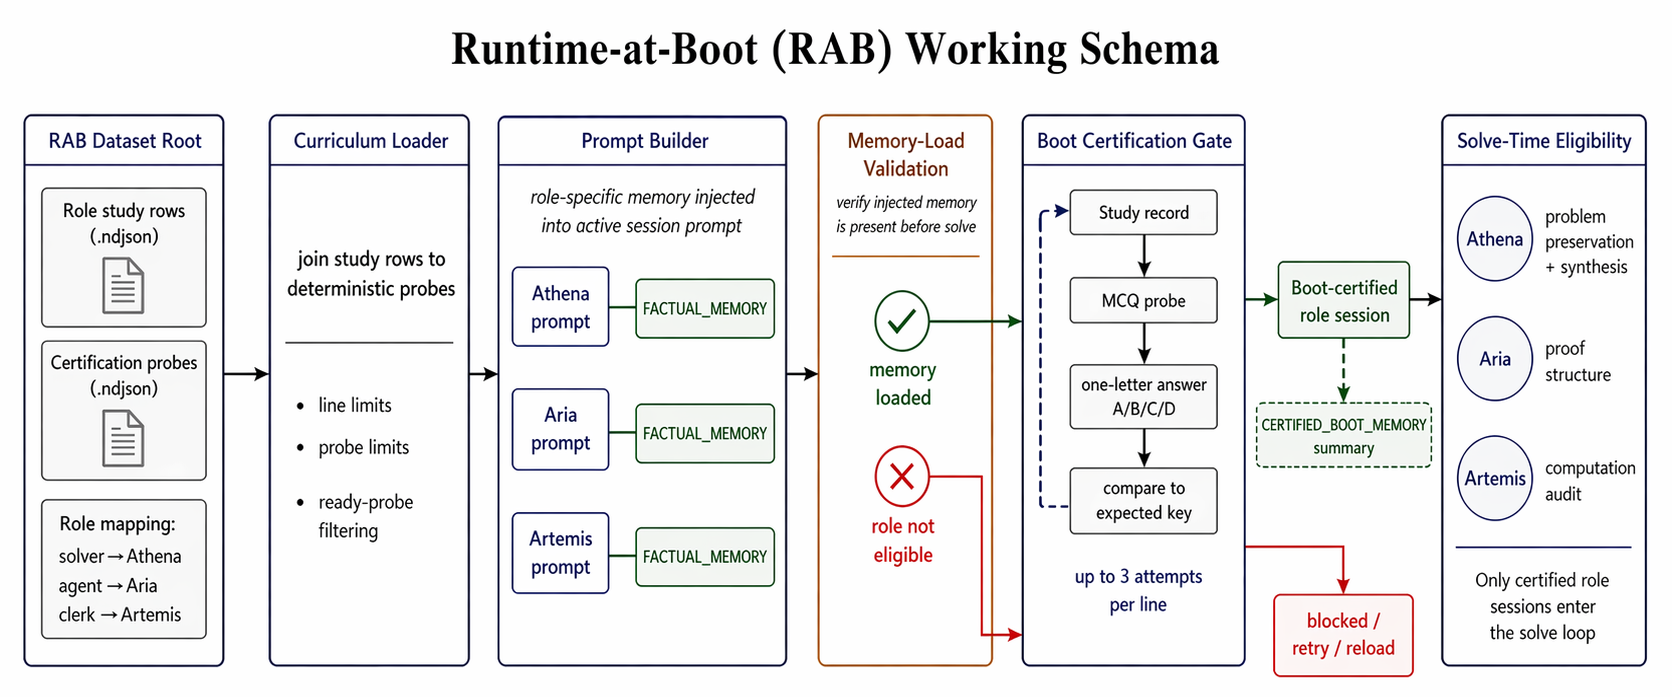
\includegraphics[width=1.06\textwidth]{diagrams/rab_schema.png}}
\caption{\rab{} working schema. Runtime-at-Boot loads role memory, validates that it is present, runs bounded certification probes, and records eligibility before solve-time inference begins.}
\label{fig:rab-working-schema}
\end{figure}

\subsection{RAB Dataset Curation}
\label{sec:rab-dataset-curation}

The \rab{} datasets are curated as role curricula, not as a single mixed memory bank. Each row is assigned a role, a short study object, and one or more certification probes. The study object teaches a reusable behavior; the probe checks whether that behavior is recoverable after boot. The paired certification probes and multiple-choice questions (MCQs) were synthetically created with GPT-5.3-Codex as a frontier artificial-intelligence model, then attached to the corresponding study rows as boot-time recall checks. This keeps curation aligned with the architecture: Athena needs problem-preservation memory, Aria needs proof-structure memory, and Artemis needs computation-audit memory. Athena and Artemis are two role views of the same Canon v2.1-derived mathematical source rather than unrelated corpora.

\subsubsection{Canon v2.1 as the Athena-Artemis curation surface}

Athena and Artemis share the same Canon v2.1-derived source dataset, but consume different surfaces of it. Canon v2.1 is the companion metadata-first distillation schema introduced in \citet{paudel2026canon}. Its purpose in AEN is not to add another answer source; it separates a mathematical item into metadata, problem text, solution structure, route obligations, and audit hooks so the same source can support multiple role curricula. Athena receives the YAML metadata surface. Candidate Canon rows are selected for complete schema structure, well-posedness, and usefulness as reusable problem-reading memory. The Athena view foregrounds taxonomy, formal objects, givens, answer contracts, family structure, reasoning components, route obligations, and solution signatures. In this role, Canon v2.1 is a route-map curriculum: it teaches Athena what must be copied, named, and protected before any compressed solution method is trusted.

Artemis receives the distilled problem-plus-solution surface from the same Canon source. That view preserves the concrete problem, the worked solution path, decisive computations, edge cases, and closeout checks. Artemis therefore does not learn a separate mathematical universe; it learns how to audit the same distilled objects that Athena sees as metadata. Where Athena sees a structured ledger for preserving the problem object, Artemis sees the corresponding proof and computation record for checking whether a proposed route actually closes.

\subsubsection{Aria proof-style curation}

Aria's dataset was curated through a different route because Aria is not the keeper of the problem ledger. Aria's job is to pressure proof structure: identify a broken implication, state the missing lemma, reject premature closure, and propose a compact repair. The curation process therefore began with proof-style reading material rather than answer-bearing problem records. Codex-assisted search was used to gather candidate proof habits from public mathematical web pages, exposition, and book-style proof discussions. These candidates were then rewritten into compact lessons: what the proof move is, why it matters, what failure it prevents, and how the pattern transfers to a new problem.

Before a lesson became Aria boot memory, it was screened against a local application programming interface (API) endpoint serving a public Qwen-family 4B checkpoint. Five diagnostic questions were written for the candidate lesson. The 4B model was queried before seeing the proposed study row. If the model already answered the questions reliably, the lesson was treated as too easy or already internal to the base model and was revised or discarded. Only when the 4B screen failed to recover the intended content was a synthetic study row created. This negative screen made the Aria dataset more valuable: the row was not merely restating what the small local model already knew, but injecting a proof habit that the boot gate could later test.

The final Aria rows therefore look different from Athena rows. They do not primarily teach a problem taxonomy. They teach proof pressure: distinguish a likelihood from a posterior, name the hinge in a temporal contradiction, preserve the raw mathematical answer before benchmark integerization, and keep a proof minimal after the route closes. The paired certification probes ask exactly those behaviors back in multiple-choice form. A passing Aria boot gate therefore means the current Aria session can recover the proof-structure discipline selected for that run.

The curation claim in this section is intentionally narrow. RAB data is role-specific study memory paired with deterministic probes. Canon v2.1 supplies the shared Athena-Artemis mathematical source: Athena receives the YAML metadata view, Artemis receives the distilled problem-plus-solution audit view, and Aria adds a separately curated proof-style curriculum after local 4B negative screening. Accuracy, timing, and certification pass counts are reported later as runtime results rather than as assumptions inside the dataset description.

\section{3-Body Reasoning Protocol}

The AEN three-body reasoning protocol is the solve-time layer that follows \rab{}. Once the required role sessions are certified, the controller algorithm builds a source-preserving problem prompt, schedules role-specific turns, records the transcript, parses candidate answers, and hands the resulting state to finalization. The roles are defined by reasoning pressure rather than by personality. \athena{} preserves the live problem object, proposes the initial route, and later reconciles the transcript. \aria{} develops proof structure: missing lemmas, alternate routes, route gaps, and repair proposals. \artemis{} applies computation pressure: arithmetic checks, edge cases, answer eligibility, and source-transcription audits. The controller algorithm then converts the role transcript into a structured finalization state rather than treating any single message as the evaluator-facing artifact.

This structure gives the protocol a clean division of labor. Problem preservation, proof construction, computation audit, synthesis, candidate parsing, and final answer emission are separate runtime duties. That separation is the point of the three-body design: each role contributes a different kind of pressure, while the controller algorithm maintains the turn order, transcript boundary, and final answer contract.

The three-body research note provides a prior three-agent framing in which a solver, critic, and arbiter communicate under fixed graphics-processing-unit budget. AEN adapts that family of ideas to the Athena/Aria/Artemis roles and to an offline integer-answer notebook surface. The important common point is not the exact name of each role, but the discipline that no single message should silently perform all functions: generate, verify, arbitrate, normalize, and emit.

\begin{table}[H]
\centering
\small
\begin{tabularx}{\linewidth}{p{0.24\linewidth}X X}
\toprule
Three-body study element & Recorded local design & AEN paper interpretation \\
\midrule
Role split & Solver, critic, and memory-grounded arbiter & \athena{} generates; \aria{} diversifies proof structure; \artemis{} audits computation and eligibility. \\
Optimization target & Stable closeout quality under fixed graphics-processing-unit budget & Measure correctness per unit complexity, not number of agents alone. \\
Memory contract & Append/tail newline-delimited JSON memory under writable working storage & Treat memory as an auditable artifact with explicit read/write boundaries. \\
Context ladder & Start at low context and promote only after clean gates & Paper-scale experiments should ramp context, tokens, and agents separately. \\
Ablation matrix & Dual, dual+memory, triad without memory, triad+memory & Required future evidence before attributing gains to the triadic protocol. \\
Closeout gates & Final-tag agreement, arbiter gate, latency and crash metrics & Finalization must report both mathematical answer and system eligibility state. \\
\bottomrule
\end{tabularx}
\caption{Methodological elements transferred from the local 3-body study into the AEN evaluation plan. These are design commitments and planned evaluation axes, not completed accuracy results.}
\label{tab:three-body-transfer}
\end{table}

\subsection{AEN Three-Body Solve Algorithm}

Algorithm~\ref{alg:aen-three-body} gives the protocol as a controller algorithm. It separates runtime eligibility, source-preserving prompt construction, bounded role interaction, candidate parsing, synthesis, and final emission.

\begin{algorithm}[H]
\caption{AEN three-body solve protocol}
\label{alg:aen-three-body}
\small
\begin{tabularx}{\linewidth}{@{}p{0.14\linewidth}X@{}}
\textbf{Input} & Problem statement \(P\); required roles \(R=\{\athena{},\aria{},\artemis{}\}\); role prompts \(I_R\); safe boot memory \(M_R\); loop budget \(L\); role/stage token budgets \(B\). \\
\textbf{State} & Certification map \(C\); transcript \(T\); parsed candidate set \(A\); objection/audit set \(O\); finalization record \(F\). \\
\textbf{Output} & Evaluator-facing integer answer \(y\) with confidence \(c\), selection mode, and artifact record; or an explicit no-eligible-answer state. \\
\end{tabularx}
\vspace{0.4em}
\begin{enumerate}
  \item Resolve offline runtime assets and record model endpoints, datasets, package versions, and artifact paths.
  \item Load the source-of-truth problem statement \(P\) and bind it to the run identifier.
  \item Run \rab{} for each required role \(r\in R\).
  \item Store the certification result for each role in \(C[r]\).
  \item If a required role is not certified, mark the run ineligible for ordinary solving and write the certification artifact.
  \item Construct the source-of-truth solve prompt \(Q\) from \(P\), \(I_R\), and \(M_R\).
  \item Initialize \(T\leftarrow\emptyset\), \(A\leftarrow\emptyset\), \(O\leftarrow\emptyset\), \(F\leftarrow\emptyset\), and \(i\leftarrow1\).
  \item While \(i\leq L\), request a bounded \athena{} route/decomposition turn using \(Q\), \(T\), and \(B\).
  \item Append the \athena{} response to \(T\) and parse route commitments and candidate answers into \(A\).
  \item Request a bounded \aria{} turn focused on proof obligations, alternate routes, and repair proposals.
  \item Request a bounded \artemis{} turn focused on arithmetic checks, edge cases, answer eligibility, and source audit.
  \item Append peer responses to \(T\); merge parsed candidate evidence into \(A\) and objections or audit flags into \(O\).
  \item Evaluate the configured closeout gate from \(A\), \(O\), role confidence, and remaining budget.
  \item If the closeout gate is open and budget remains, compress the current state, set \(i\leftarrow i+1\), and continue.
  \item Send the compact peer-report state to \athena{} for synthesis and parse the controller-provided boxed-confidence candidate slot into \(F\).
  \item Select the emitted candidate from \(A\cup F\): strict three-role agreement, then two-role majority, then highest-confidence eligible candidate.
  \item Emit \(y\), confidence \(c\), selection mode, transcript path, prompt payloads, and finalization artifact.
\end{enumerate}
\end{algorithm}

\begin{figure}[H]
\centering
\makebox[\textwidth][c]{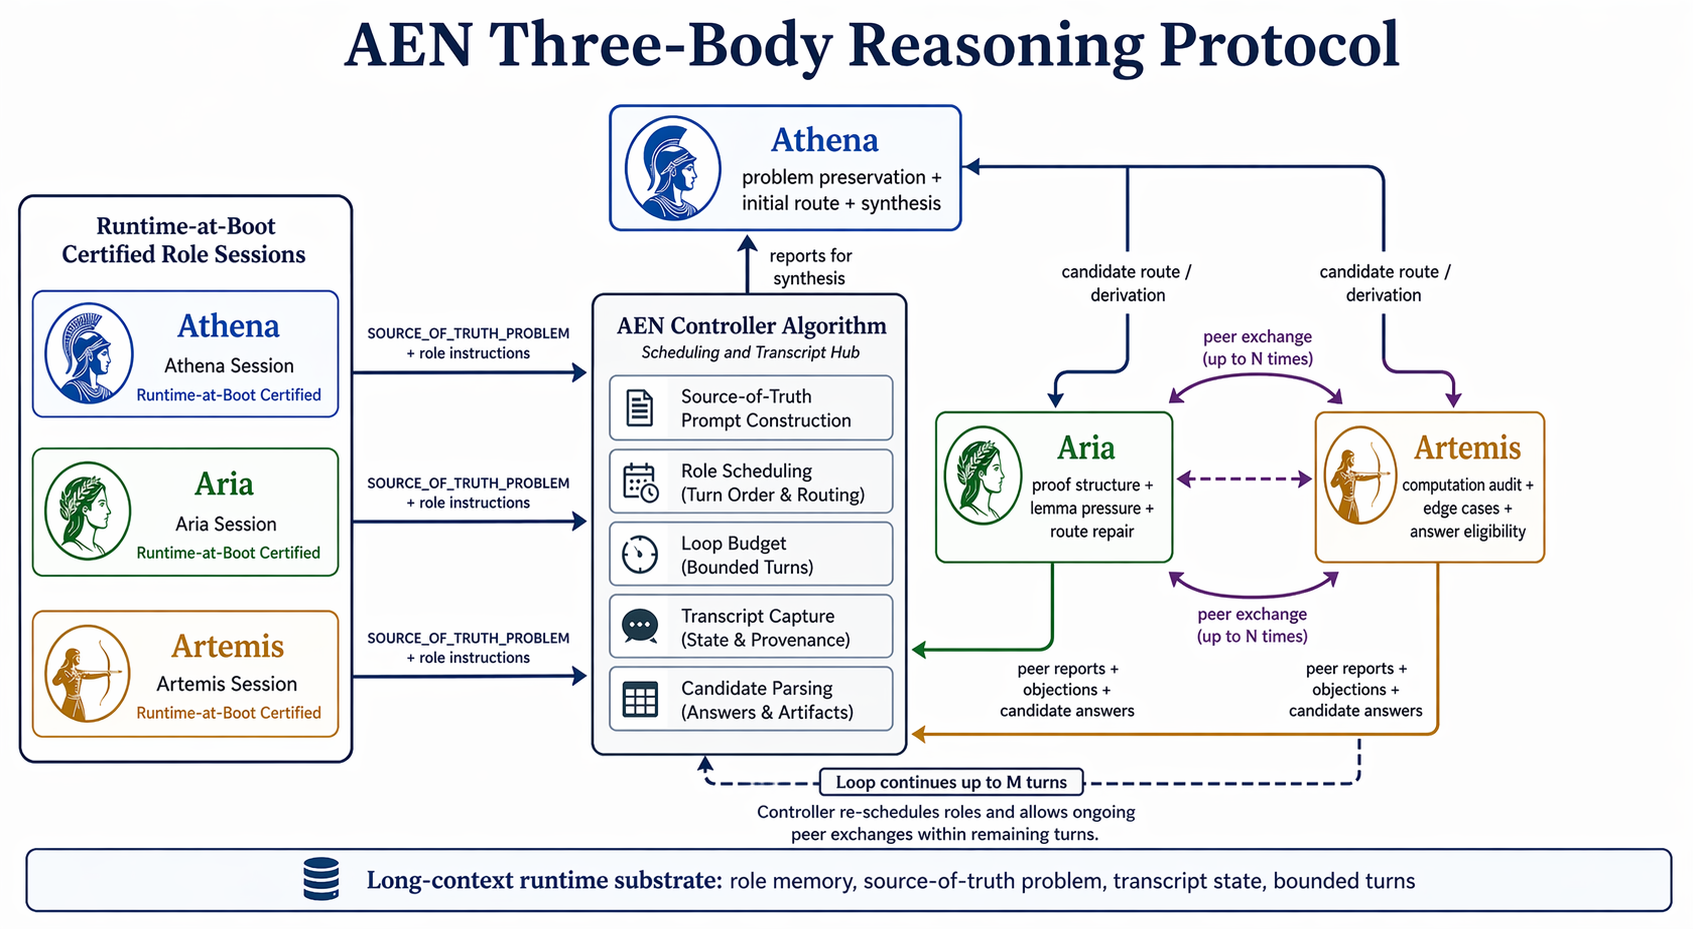
\includegraphics[width=1.08\textwidth]{diagrams/3_body_reasoning_protocol.png}}
\caption{Three-body reasoning protocol after \rab{} certification. The AEN controller algorithm schedules \athena{}, \aria{}, and \artemis{} as separate reasoning-pressure roles, records the transcript state, and passes parsed candidates and role evidence into finalization.}
\label{fig:three-body-reasoning-protocol}
\end{figure}

\begin{table}[t]
\centering
\small
\begin{tabularx}{\linewidth}{p{0.24\linewidth}X}
\toprule
Invariant & Meaning \\
\midrule
Role eligibility is explicit & A role is not silently assumed available; the run records whether its \rab{} gate passed. \\
Solve memory is sanitized & Certification data and solve-time memory are separate objects; answer-bearing evaluation data should not enter prompts. \\
Turns are bounded & The controller chooses when roles speak and how much context each receives. \\
Verification is typed & The system distinguishes checked agreement, weak agreement, unverified candidates, and unavailable answers. \\
Finalization is controller-managed & The wrapper-facing answer is emitted by the controller from parsed candidate state, not by model prose alone. \\
Artifacts are first-class & Prompt payloads, transcripts, finalization mode, and emitted answers are part of the result. \\
\bottomrule
\end{tabularx}
\caption{Core AEN protocol invariants.}
\label{tab:invariants}
\end{table}

\subsection{Controller Algorithm and Finalization}

Finalization is the step where a mathematical trace becomes an evaluator-facing answer. The present AEN implementation is optimized for integer-answer validation because several important language-model mathematical-reasoning test surfaces use exact integer answers. American Invitational Mathematics Examination (AIME) contest statements specify answers as integers from \(000\) to \(999\) inclusive \citep{aops2000aime}. The Artificial Intelligence Mathematical Olympiad (AIMO) Progress Prize has likewise used integer-normalized answer fields; the AIMO3 announcement describes the move to five-digit answers, making the answer space larger while preserving an integer wrapper \citep{aimoprize2025third}. Harvard--MIT Mathematics Tournament (HMMT) should not be described as integer-only: its testing page describes individual tests as single-value short-answer exams, and its acceptable-answer rules allow fractions, radicals, trigonometric expressions, and complete lists when appropriate \citep{hmmtTesting,hmmtAcceptableAnswers}.

This means that the integer wrapper is an engineering optimization, not a universal definition of mathematical reasoning. For AIME/AIMO-style validation, a single normalized integer gives the controller a clean target: parse candidate integers, compare role agreement, apply confidence and eligibility gates, and write one wrapper-facing answer. For a rational-answer, expression-answer, list-answer, or proof-graded benchmark, the same controller algorithm can keep the role protocol while replacing the parser, equivalence checker, and final emission schema. In that sense, AEN is optimized for integer answers because that is the most efficient validation interface for the current target experiments, and the optimization is deliberately local to the finalization layer.

The controller supplies a boxed-confidence closeout template for \athena{} to fill during synthesis or finalization: \texttt{\textbackslash boxed\{[integer\_value]\}} followed by \texttt{\_confidence:[0-100]}. Peer turns do not own this wrapper. \aria{} and \artemis{} contribute support, objections, alternate routes, audit evidence, and confidence signals; \athena{} reconciles those reports into a controller-facing candidate; the controller algorithm parses the candidate, gates it, records the selection mode, and emits the wrapper-facing answer.

The candidate-selection rule is deliberately explicit. If \athena{}, \aria{}, and \artemis{} emit the same integer candidate, the controller records strict three-role consensus and emits that value. If exactly two roles agree and the third role disagrees or is unavailable, the controller records a majority-vote fallback and emits the shared value. If no two roles emit the same integer, the controller records a highest-confidence fallback and emits the highest-confidence eligible candidate. These fallback modes are not semantic proof certificates; they are controller labels that tell the reader how the wrapper-facing answer was selected.

This design keeps malformed answers from becoming accidental submissions. A model may write a plausible sentence around an answer, but the controller algorithm records whether the emitted artifact came from strict agreement, majority agreement, or highest-confidence fallback. The finalization artifact therefore reports both the selected integer and the route by which that integer became eligible for emission.

The runtime envelope records that \texttt{CONTEXT\_RUNTIME\_BOOT\_INJECTION\_MODE} defaults to \texttt{safe\_prompt\_memory}; solve prompts receive a compact sanitized runtime memory surface rather than the full factual or certified boot memory. It also records explicit controller budgets: Athena opening turns at 900 max generated tokens, Athena synthesis turns at 768, and Aria/Artemis exchange/report turns at 768, with \texttt{GLOBAL\_MAX\_TURN\_TOKENS = 0} interpreted as using those role/stage budgets. This is useful because it turns ``bounded dialogue'' into a reproducible runtime contract.

\clearpage
\begin{figure}[H]
\centering
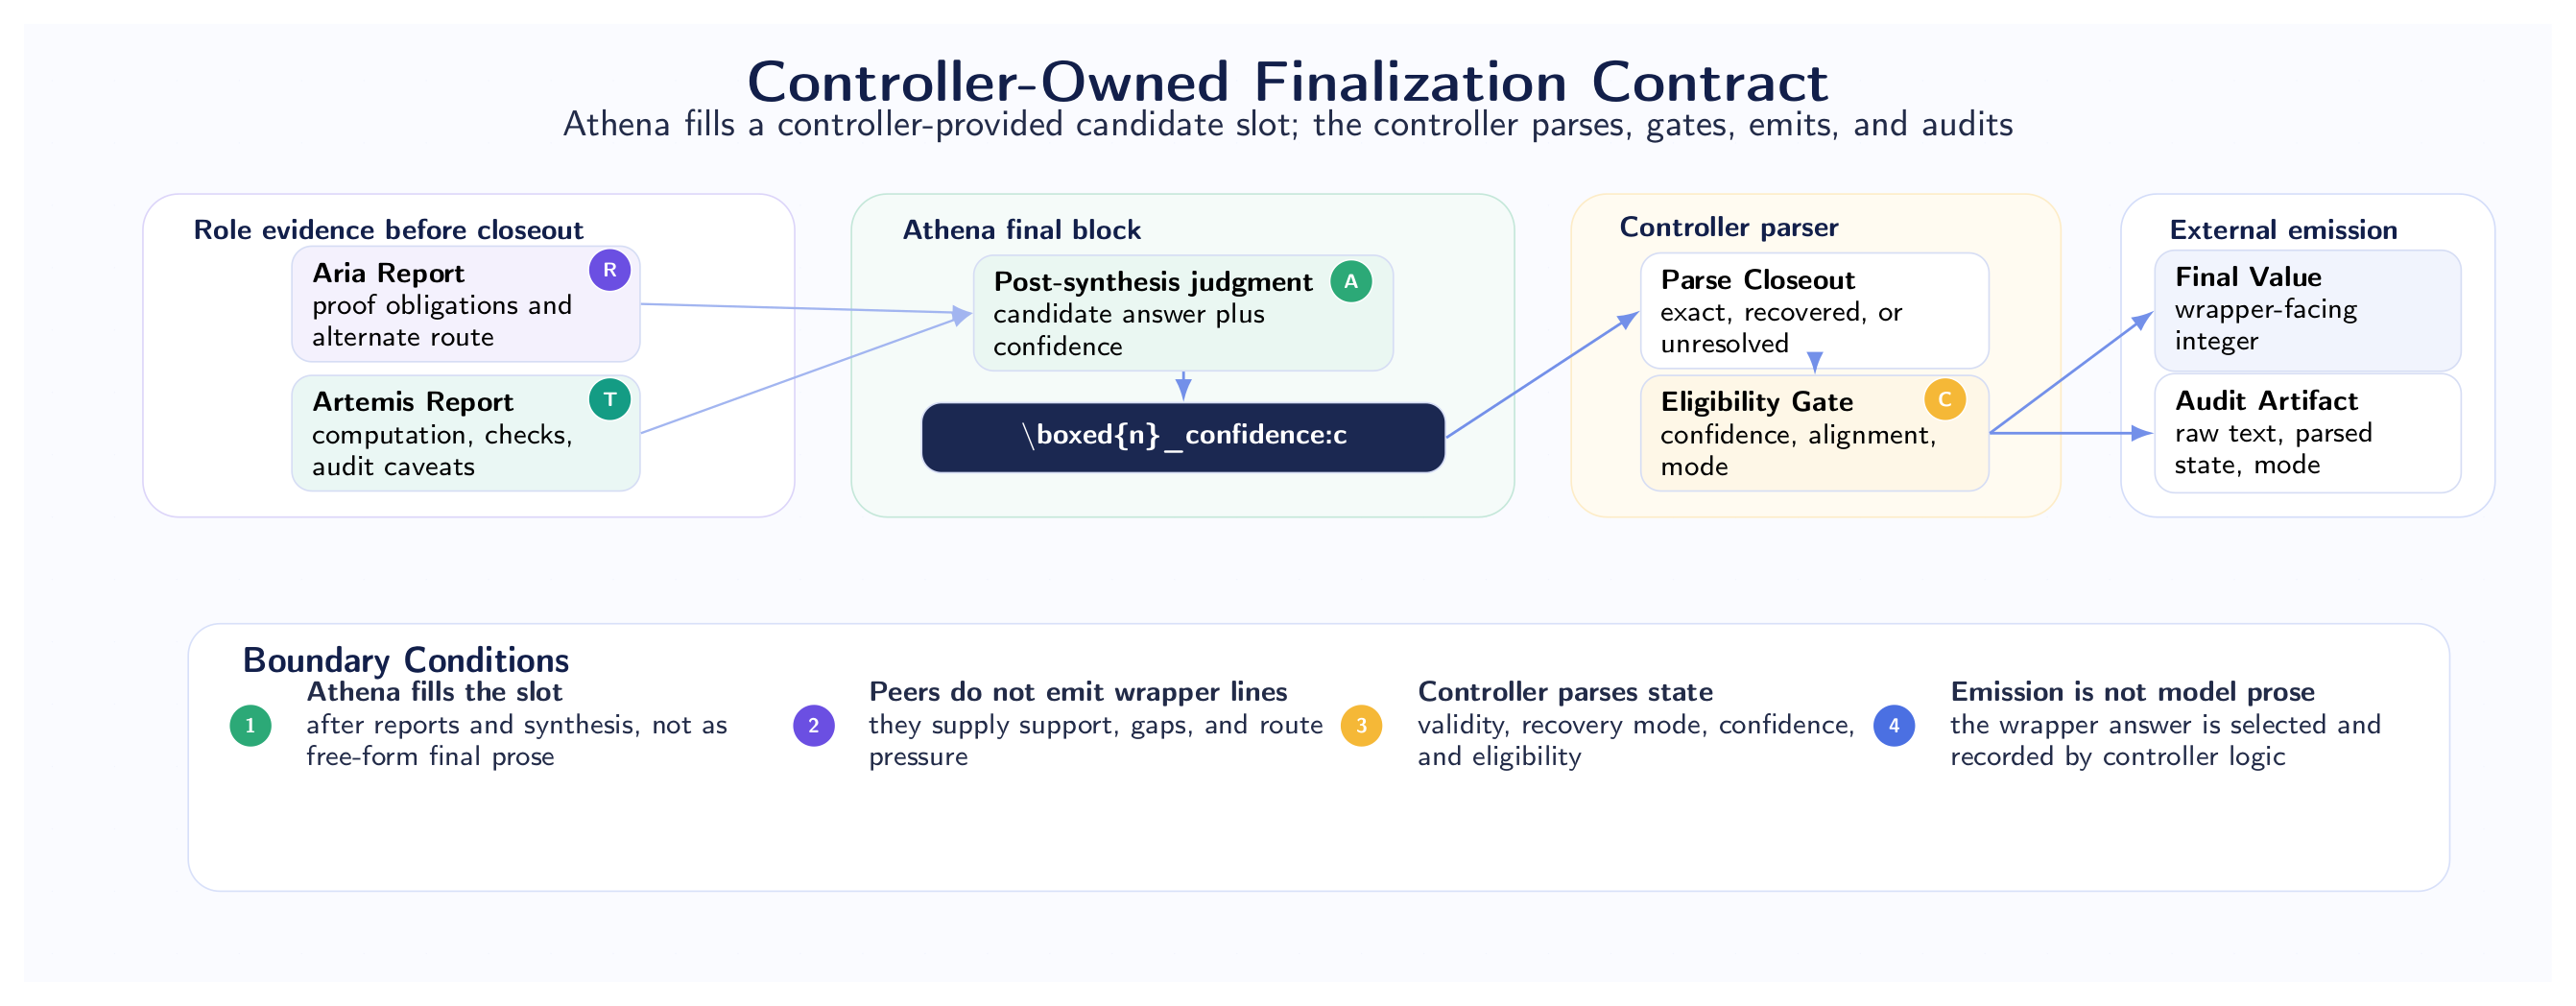
\includegraphics[width=0.92\textwidth]{diagrams/controller_finalization_contract.png}
\caption{Controller-owned finalization contract. Peer reports provide role evidence, \athena{} fills the controller-provided candidate slot, and the controller parses, gates, emits, and audits the wrapper-facing answer.}
\label{fig:controller-finalization-contract}
\end{figure}

\vspace{-0.8em}
\paragraph{Instruction-append turn discipline.}

The turn discipline below is the controller's prompt-append schedule. Each row adds only the phase-specific pressure needed for the next role, while the shared envelope preserves role, source problem, state, route, loop protocol, and output contract.

\begin{table}[H]
\centering
\footnotesize
\setlength{\tabcolsep}{5pt}
\renewcommand{\arraystretch}{1.16}
\begin{tabularx}{\textwidth}{>{\raggedright\arraybackslash}p{0.19\textwidth}>{\raggedright\arraybackslash}p{0.31\textwidth}X}
\toprule
Phase & Controller append & Visible contract \\
\midrule
Shared envelope & Role, source-of-truth problem, state, route, loop protocol, output contract. & No role may change the problem object or emit a final answer unless its phase allows it. \\
\athena{} open & Opening template. & Problem setup, Canon v2.1 ledger, route options, preferred route; no boxed answer. \\
\aria{} exchange 1 & Proof-route and lemma pressure. & Accept route, state lemma, build proof, name obstruction, hand off to \artemis{}. \\
\artemis{} exchange 1 & Audit and computation pressure. & Challenge or accept, check computation, test edge cases, give audit verdict. \\
\aria{} later exchange & Repair-or-close instruction. & Repair or reject objections, strengthen route, state remaining gap, mark candidate status. \\
\artemis{} later exchange & Independent closeout audit. & Stress route, verify arithmetic, check boundaries, confirm or block closeout. \\
Peer reports & Report template. & First line is \textit{Report Verdict}; include answer, confidence, status, and checklist. \\
\athena{} synthesis & Peer reports plus candidate slot. & Reconcile objections and fill one boxed-confidence candidate. \\
\athena{} finalization & Controller one-line final prompt. & Exactly \texttt{\textbackslash boxed\{integer\}\_confidence:[0-100]}; no prose. \\
\bottomrule
\end{tabularx}
\caption{Instruction-append turn discipline. The shared envelope is constant; each phase appends one small role-specific contract.}
\label{tab:instruction-append-turn-discipline}
\end{table}

\subsection{Runtime Knobs}

AEN is not a fixed prompt template. It is a controller architecture with explicit runtime knobs. The point of naming these knobs before evaluation is methodological: a result should be read together with the exact loop, exchange, closeout, and token-budget settings that produced it. Changing these values can change accuracy, wall time, transcript length, and failure mode without changing model weights.

\begin{table}[H]
\centering
\footnotesize
\setlength{\tabcolsep}{4pt}
\renewcommand{\arraystretch}{1.08}
\begin{tabularx}{\textwidth}{>{\raggedright\arraybackslash}p{0.38\textwidth}>{\raggedright\arraybackslash}p{0.13\textwidth}X}
\toprule
Runtime knob & Value & Turned surface \\
\midrule
\texttt{GLOBAL\_MAX\_BIG\_LOOPS} & \texttt{1} & Outer solve-loop ceiling. \\
\texttt{GLOBAL\_MIN\_BIG\_LOOP\_FOR\_CLOSEOUT} & \texttt{1} & Earliest loop where closeout is permitted. \\
\texttt{GLOBAL\_CLOSEOUT\_CONFIDENCE\_PCT} & \texttt{85} & Parsed-confidence gate for closeout eligibility. \\
\texttt{GLOBAL\_INNER\_TOTAL\_EXCHANGES} & \texttt{3} & Aria--Artemis exchange depth inside each loop. \\
\texttt{GLOBAL\_MAX\_TURN\_TOKENS} & \texttt{0} & Global turn cap override; zero defers to role and phase caps. \\
\texttt{ATHENA\_MAX\_TOKENS} & \texttt{8192} & Athena role-level generation ceiling. \\
\texttt{ARIA\_MAX\_TOKENS} & \texttt{12288} & Aria role-level generation ceiling. \\
\texttt{ARTEMIS\_MAX\_TOKENS} & \texttt{12288} & Artemis role-level generation ceiling. \\
\texttt{ATHENA\_OPEN\_MAX\_TOKENS} & \texttt{4096} & Athena opening/decomposition budget. \\
\texttt{ATHENA\_SYNTHESIS\_MAX\_TOKENS} & \texttt{2048} & Athena synthesis budget after peer reports. \\
\texttt{ATHENA\_FINAL\_MAX\_TOKENS} & \texttt{128} & Athena final one-line emission budget. \\
\texttt{PEER\_EXCHANGE\_MAX\_TOKENS} & \texttt{4096} & Shared peer exchange cap. \\
\texttt{PEER\_REPORT\_MAX\_TOKENS} & \texttt{4096} & Shared peer report cap. \\
\texttt{ARIA\_EXCHANGE\_MAX\_TOKENS} & \texttt{4096} & Aria exchange cap. \\
\texttt{ARTEMIS\_EXCHANGE\_MAX\_TOKENS} & \texttt{4096} & Artemis exchange cap. \\
\texttt{ARIA\_REPORT\_MAX\_TOKENS} & \texttt{4096} & Aria report cap. \\
\texttt{ARTEMIS\_REPORT\_MAX\_TOKENS} & \texttt{4096} & Artemis report cap. \\
\texttt{GLOBAL\_SHOW\_STREAMING} & \texttt{False} & Live text display toggle. \\
\texttt{GLOBAL\_PRINT\_PROGRESS\_LINES} & \texttt{True} & Controller progress-line toggle. \\
\texttt{GLOBAL\_ENABLE\_TOKEN\_STREAMING} & \texttt{True} & Runtime token-streaming toggle. \\
\texttt{GLOBAL\_STREAM\_PRINT\_ROLE\_PREFIX} & \texttt{True} & Role-prefix display for streamed tokens. \\
\texttt{GLOBAL\_STREAM\_TOKEN\_MODE} & \texttt{word} & Streaming display granularity. \\
\bottomrule
\end{tabularx}
\caption{AEN runtime knobs. Only turnable loop, exchange, token-budget, and observability settings are listed.}
\label{tab:runtime-knobs}
\end{table}

These knobs define the difference between a constrained diagnostic run and a ceiling-seeking run. A compressed notebook may lower generation budgets, reduce peer exchanges, and use a single loop to fit a wall-clock envelope. A larger-resource run may increase loop count, raise per-turn caps, and allow more peer exchanges before synthesis. Both are still AEN runs, but they test different regions of the same controller.

\clearpage
\section{Evaluation and Diagnostics}

The evaluation methodology separates structural validity from mathematical strength. A system can be structurally valid and mathematically weak; it can also solve local problems while being unsafe for an external evaluator. AEN therefore reports multiple artifact classes rather than a single headline number.

All runs in this section were executed as offline notebook evaluations. Required Python wheels for vLLM support and related runtime dependencies were supplied through an attached Kaggle wheel dataset rather than live package downloads; the public wheel bundle is available as the Kaggle dataset \citet{paudel2026wheels}. The reported artifacts therefore measure the notebook path under offline execution: attached wheel installation, attached boot datasets, runtime certification, transcript export, scoring, and artifact bundling.

The first test surface is our own Vault of Echoes (VoE) dataset: a lore-infused 25-question puzzle corpus designed to stress transcript reading, puzzle-state preservation, answer normalization, and controller discipline. The Vault of Echoes interface and transcript methodology are described in the companion user-interface-native benchmark record, published on 12 January 2026 \citep{paudel2026uinative}. The public AEN runtime dataset is the Kaggle RuntimeAtBoot dataset \citep{paudel2026runtimeatbootdataset}, available at \url{https://www.kaggle.com/datasets/aadityapaudel/runtimeatboot}. This makes VoE a deployment-adjacent diagnostic rather than an external contest benchmark: it is useful for understanding controller behavior, runtime cost, memory recall, and answer-normalization pressure.

The second test surface is American Invitational Mathematics Examination (AIME)-style contest mathematics. AIME is a cleaner exact-integer benchmark target than VoE because the evaluator-facing answer is already a single normalized integer. AEN therefore reports VoE diagnostics and AIME diagnostics separately. VoE tells us how the controller behaves on lore-heavy puzzle tasks with normalization pressure; AIME tells us how the constrained notebook behaves on held-out contest-style integer problems.

The VoE and AIME diagnostics were not run under identical generation envelopes. The fresh VoE run used an earlier high-context one-loop schema: Athena opening was capped at 8192 generated tokens, Aria and Artemis exchange turns at 4096, peer reports and Athena synthesis at 2048, and final emission at 512. The later contest-math notebook used a more compressed competition envelope. The two surfaces should therefore be read as separate diagnostics rather than as one direct accuracy comparison.

VoE is tested under two premises. First, AEN is run as a fresh architecture test: the roles receive the curated boot memory described in Section~\ref{sec:rab-dataset-curation}, but the solve prompt does not contain the canonical solutions for the VoE test rows. This condition measures how the triadic runtime performs when the models must solve from the problem statement, role memory, peer exchange, and controller finalization alone. Second, because VoE is an internal benchmark whose canonical solutions are available to the authors, AEN is run as a memory-certified replay. In that condition, the canonical solution rows for the ten missed cases are loaded as answer-bearing boot memory and certified before solving. A successful replay has a narrow interpretation: it tests whether \rab{} can make supplied solution memory active enough to affect the emitted answer.

The UI-native comparison surface was recorded in January 2026 and published on 12 January 2026 \citep{paudel2026uinative}. It was a one-shot controlled chat benchmark over the same 25-question VoE corpus, using then-available frontier public chat models together with lower-latency instant models. The comparison is therefore useful as a trusted workbook for the puzzle surface, while the AEN runs below remain architecture diagnostics rather than a public leaderboard claim.

\subsection{Fresh Vault of Echoes Run (No Answer Memory)}

The fresh VoE run evaluates the triadic controller on the public 25-case VoE surface without answer-bearing golden prompt rows for the test cases. Runtime-at-Boot still certifies the role sessions, but the solve prompt does not carry the missed-case golden answers that are used in the later memory-loaded condition. Under this condition AEN scores 15/25 on the canonical comparison surface. In the trusted workbook associated with the user-interface-native VoE record, this places the fresh AEN run at the same solved-count level as GPT 5.2 and Gemini 3 on this 25-question corpus.

The attached-test summary records 25 cases, \path{runtime_at_boot_passed: true}, and total wall time 12336.25 seconds, about 3.43 hours for the Kaggle workflow. The high-context turn schema has a generated-token cap total of 31,232 per problem before prompt and context tokens are counted. The measured average total token load in the full log is approximately 466,283 tokens per problem, which explains why the later contest-math notebook was compressed more aggressively.

\begin{figure}[H]
\centering
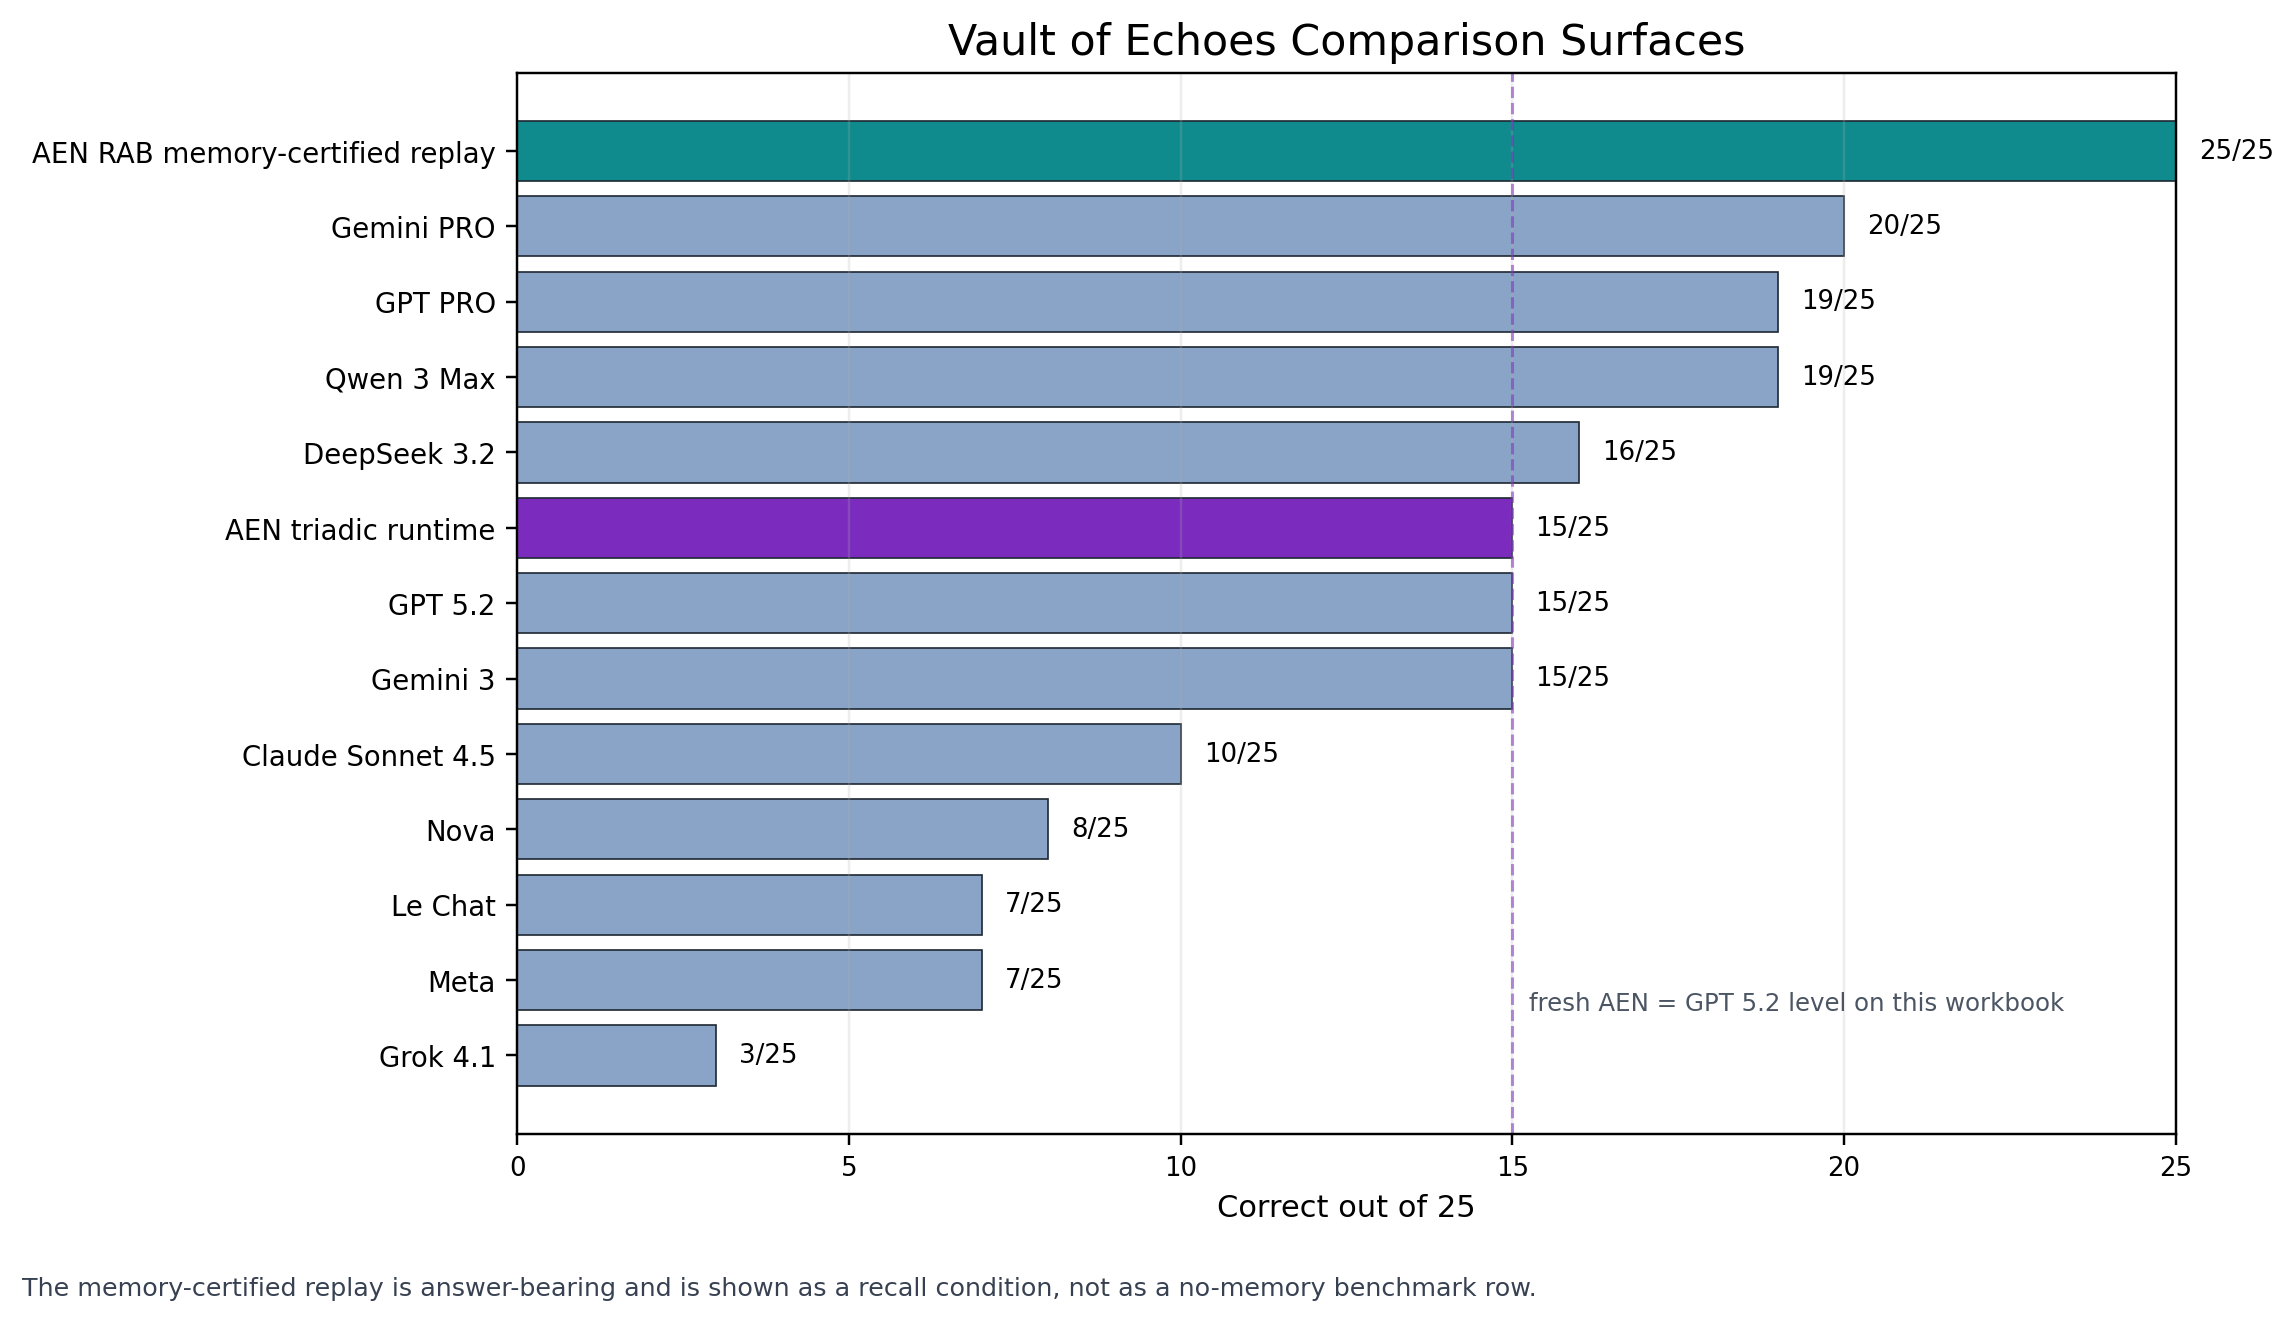
\includegraphics[width=\linewidth]{diagrams/voe_trusted_benchmark_comparison.png}
\caption{Vault of Echoes comparison surfaces. The fresh AEN triadic runtime is scored as 15/25 on the no-answer-memory surface and is plotted against the trusted workbook associated with the companion VoE record; the memory-certified replay is shown separately because it is answer-bearing.}
\label{fig:voe-trusted-benchmark-comparison}
\end{figure}

\begin{figure}[H]
\centering
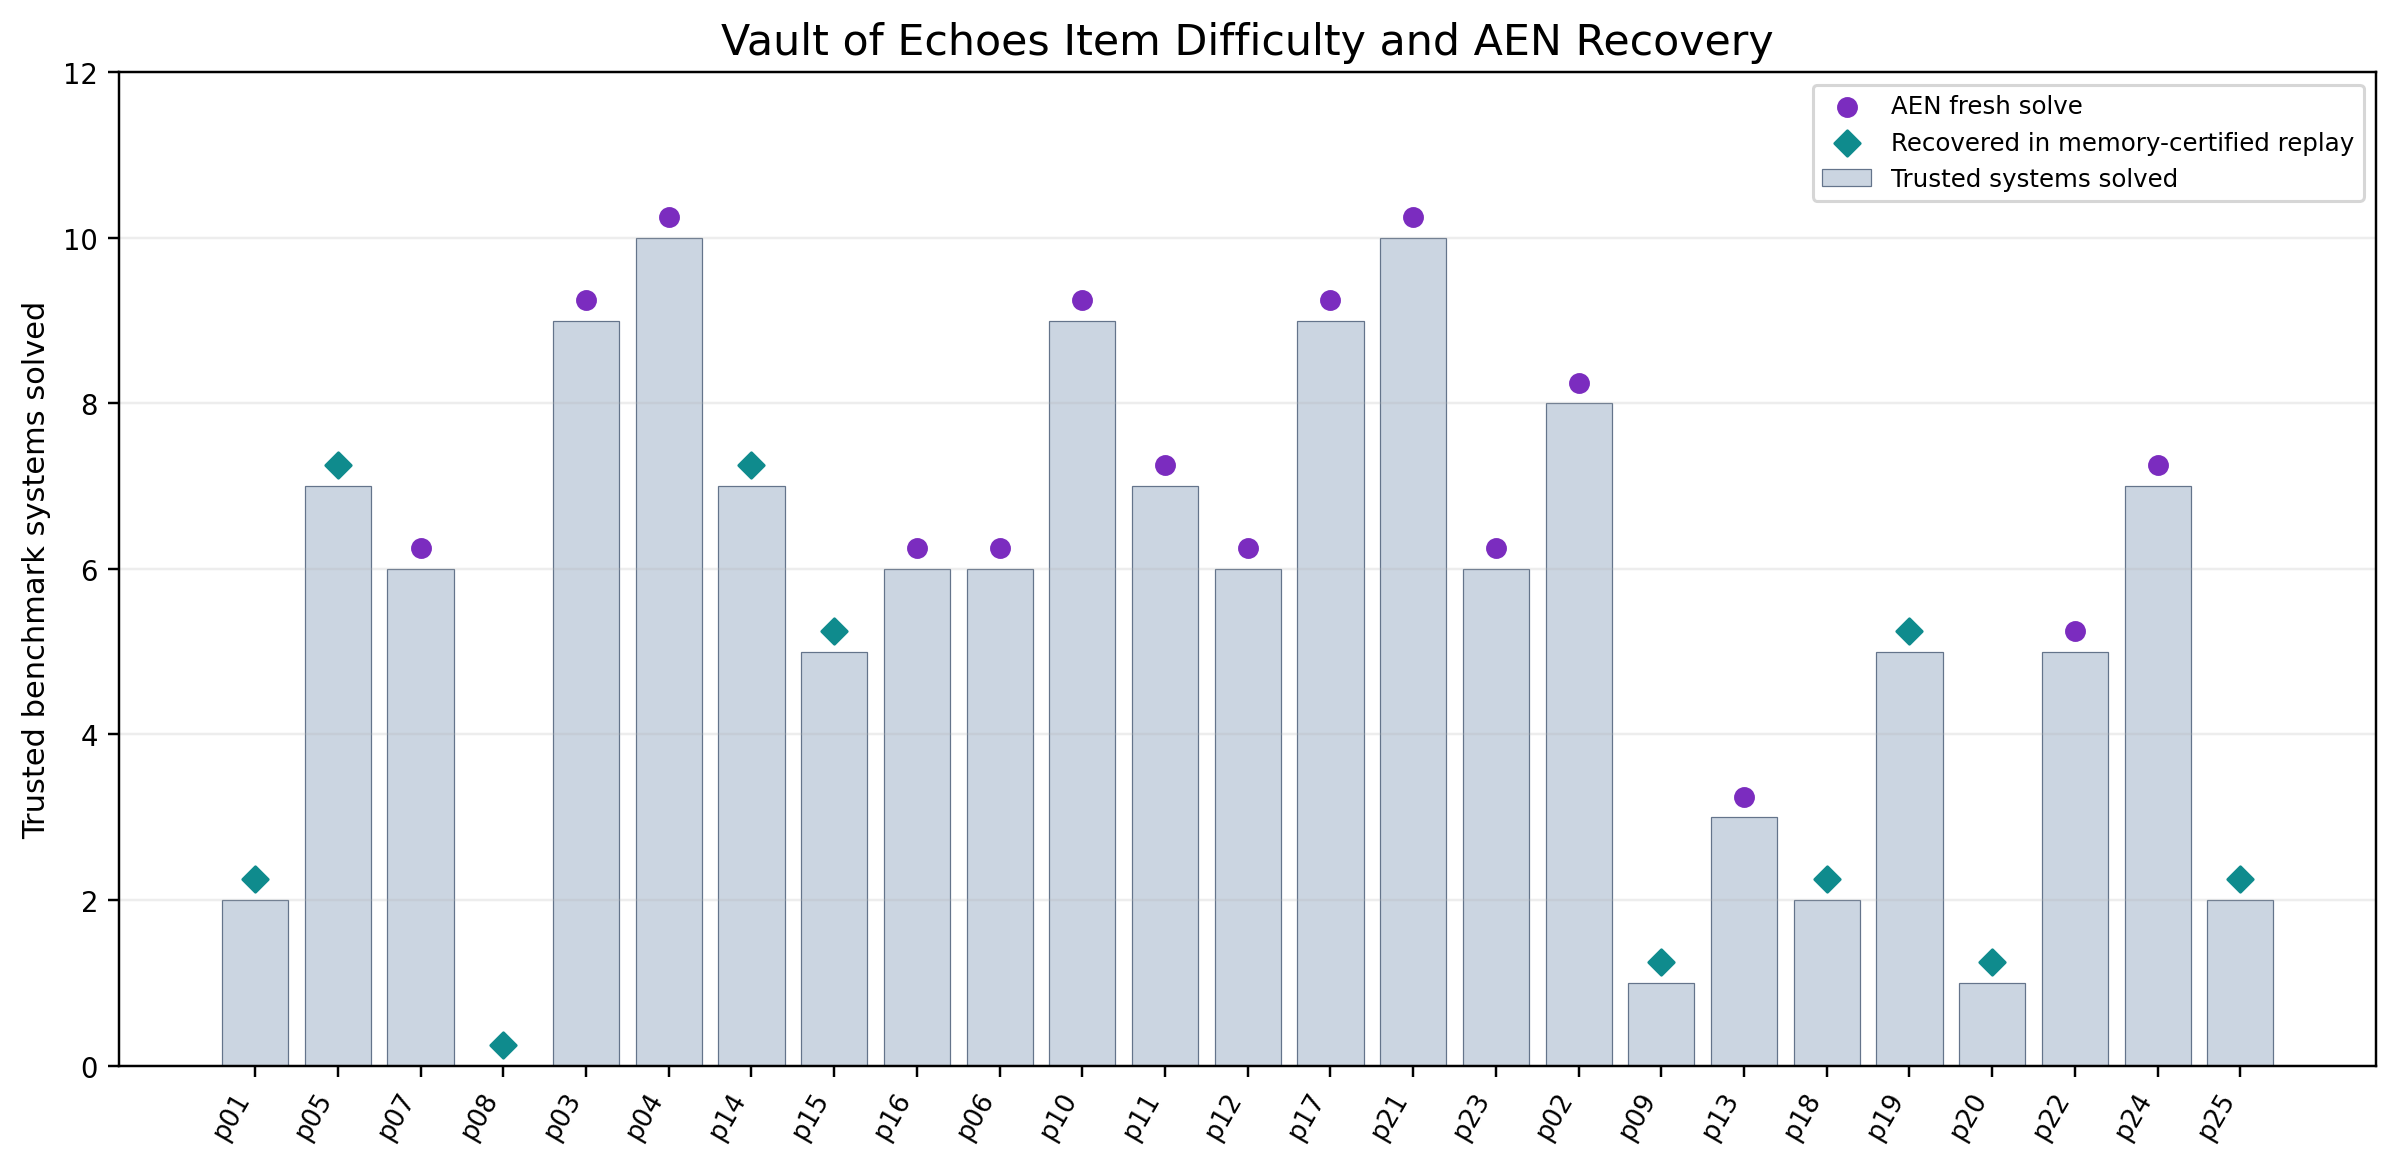
\includegraphics[width=\linewidth]{diagrams/voe_problem_difficulty_comparison.png}
\caption{Vault of Echoes item-difficulty comparison. Bars show how many trusted UI-native benchmark systems solved each puzzle; purple markers indicate fresh AEN solves, while teal markers indicate cases recovered in the memory-certified replay.}
\label{fig:voe-problem-difficulty-comparison}
\end{figure}

\begin{figure}[H]
\centering
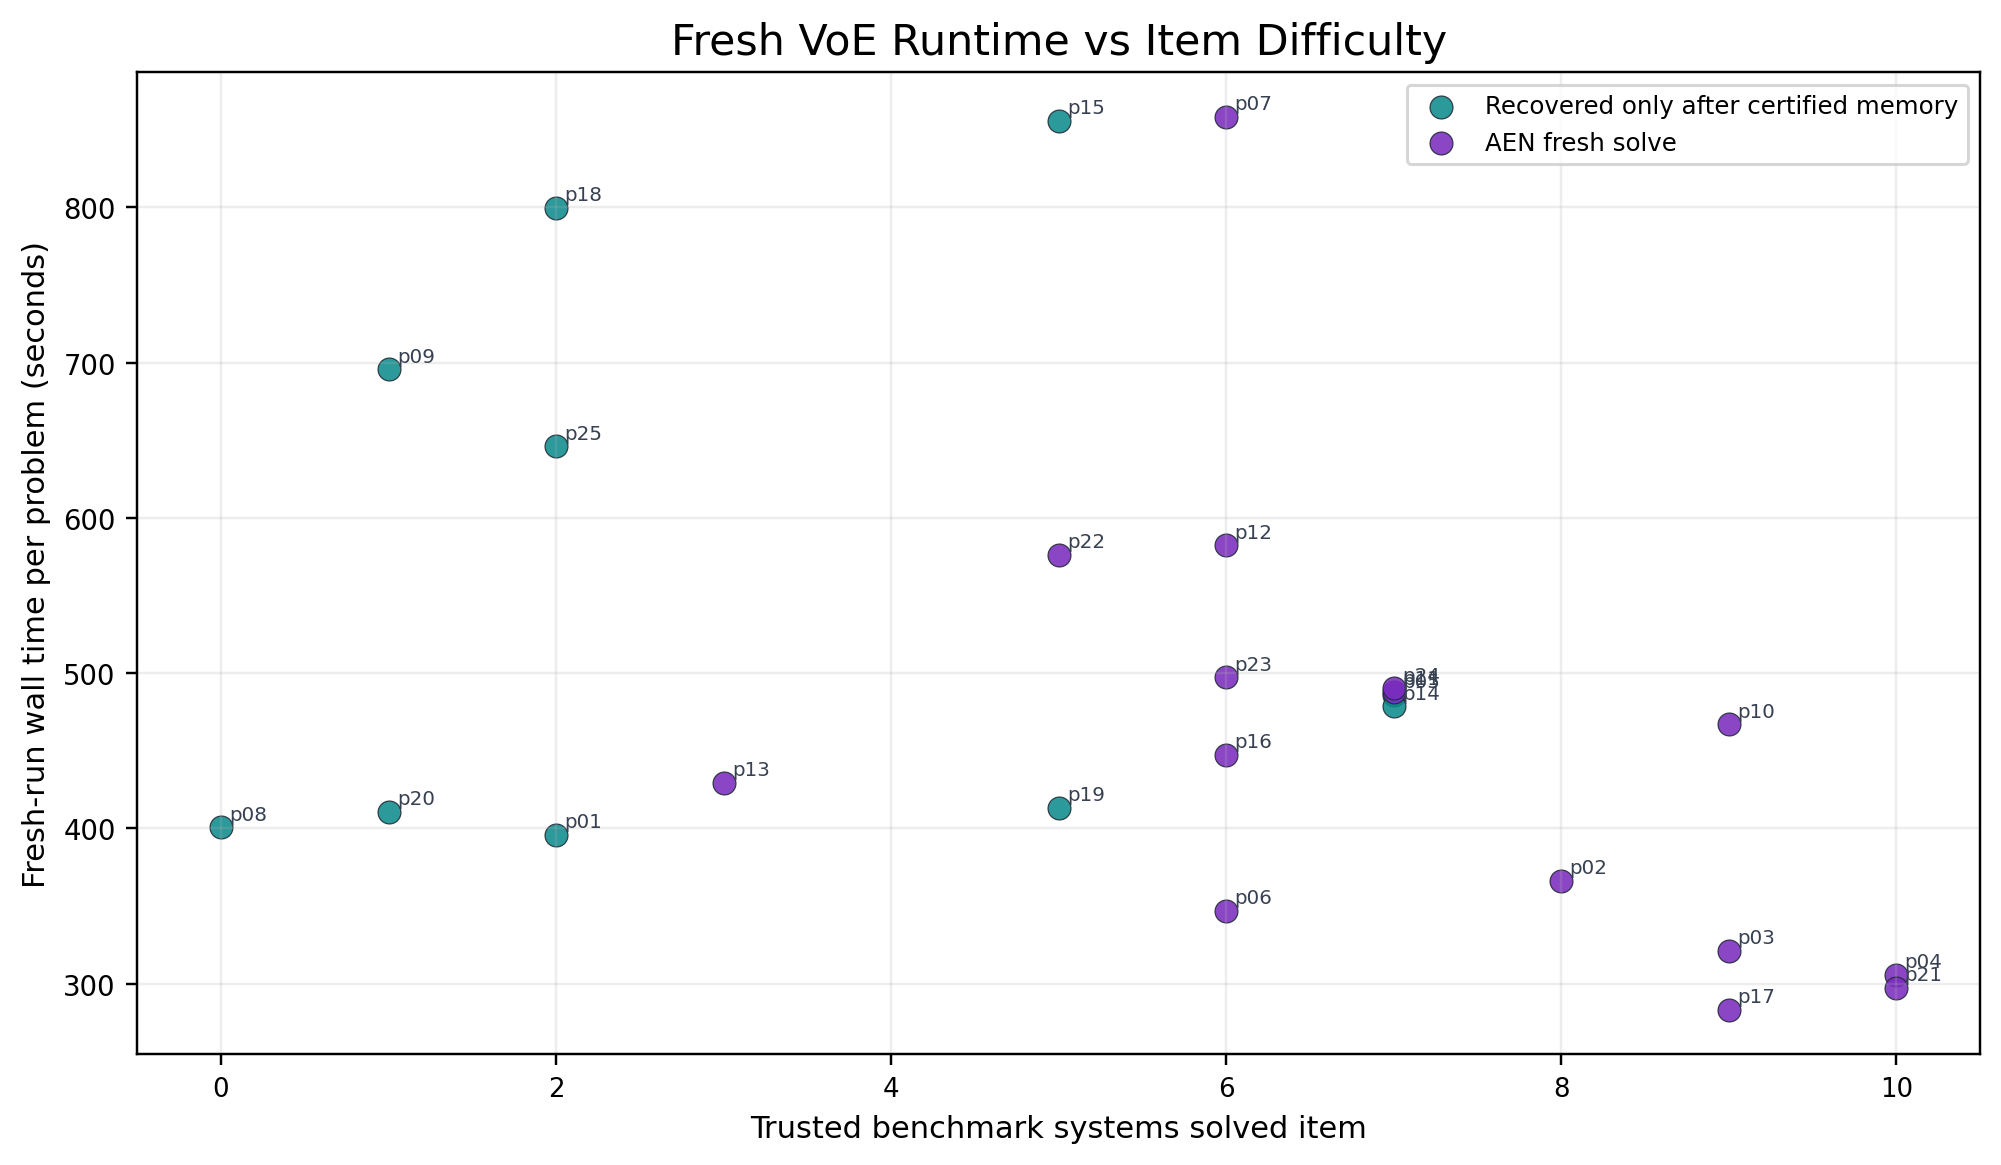
\includegraphics[width=\linewidth]{diagrams/voe_aen_runtime_vs_difficulty.png}
\caption{Fresh VoE runtime against trusted-workbook item difficulty. This plot relates per-problem AEN wall time to the number of trusted benchmark systems that solved the same item.}
\label{fig:voe-aen-runtime-vs-difficulty}
\end{figure}

\begin{figure}[H]
\centering
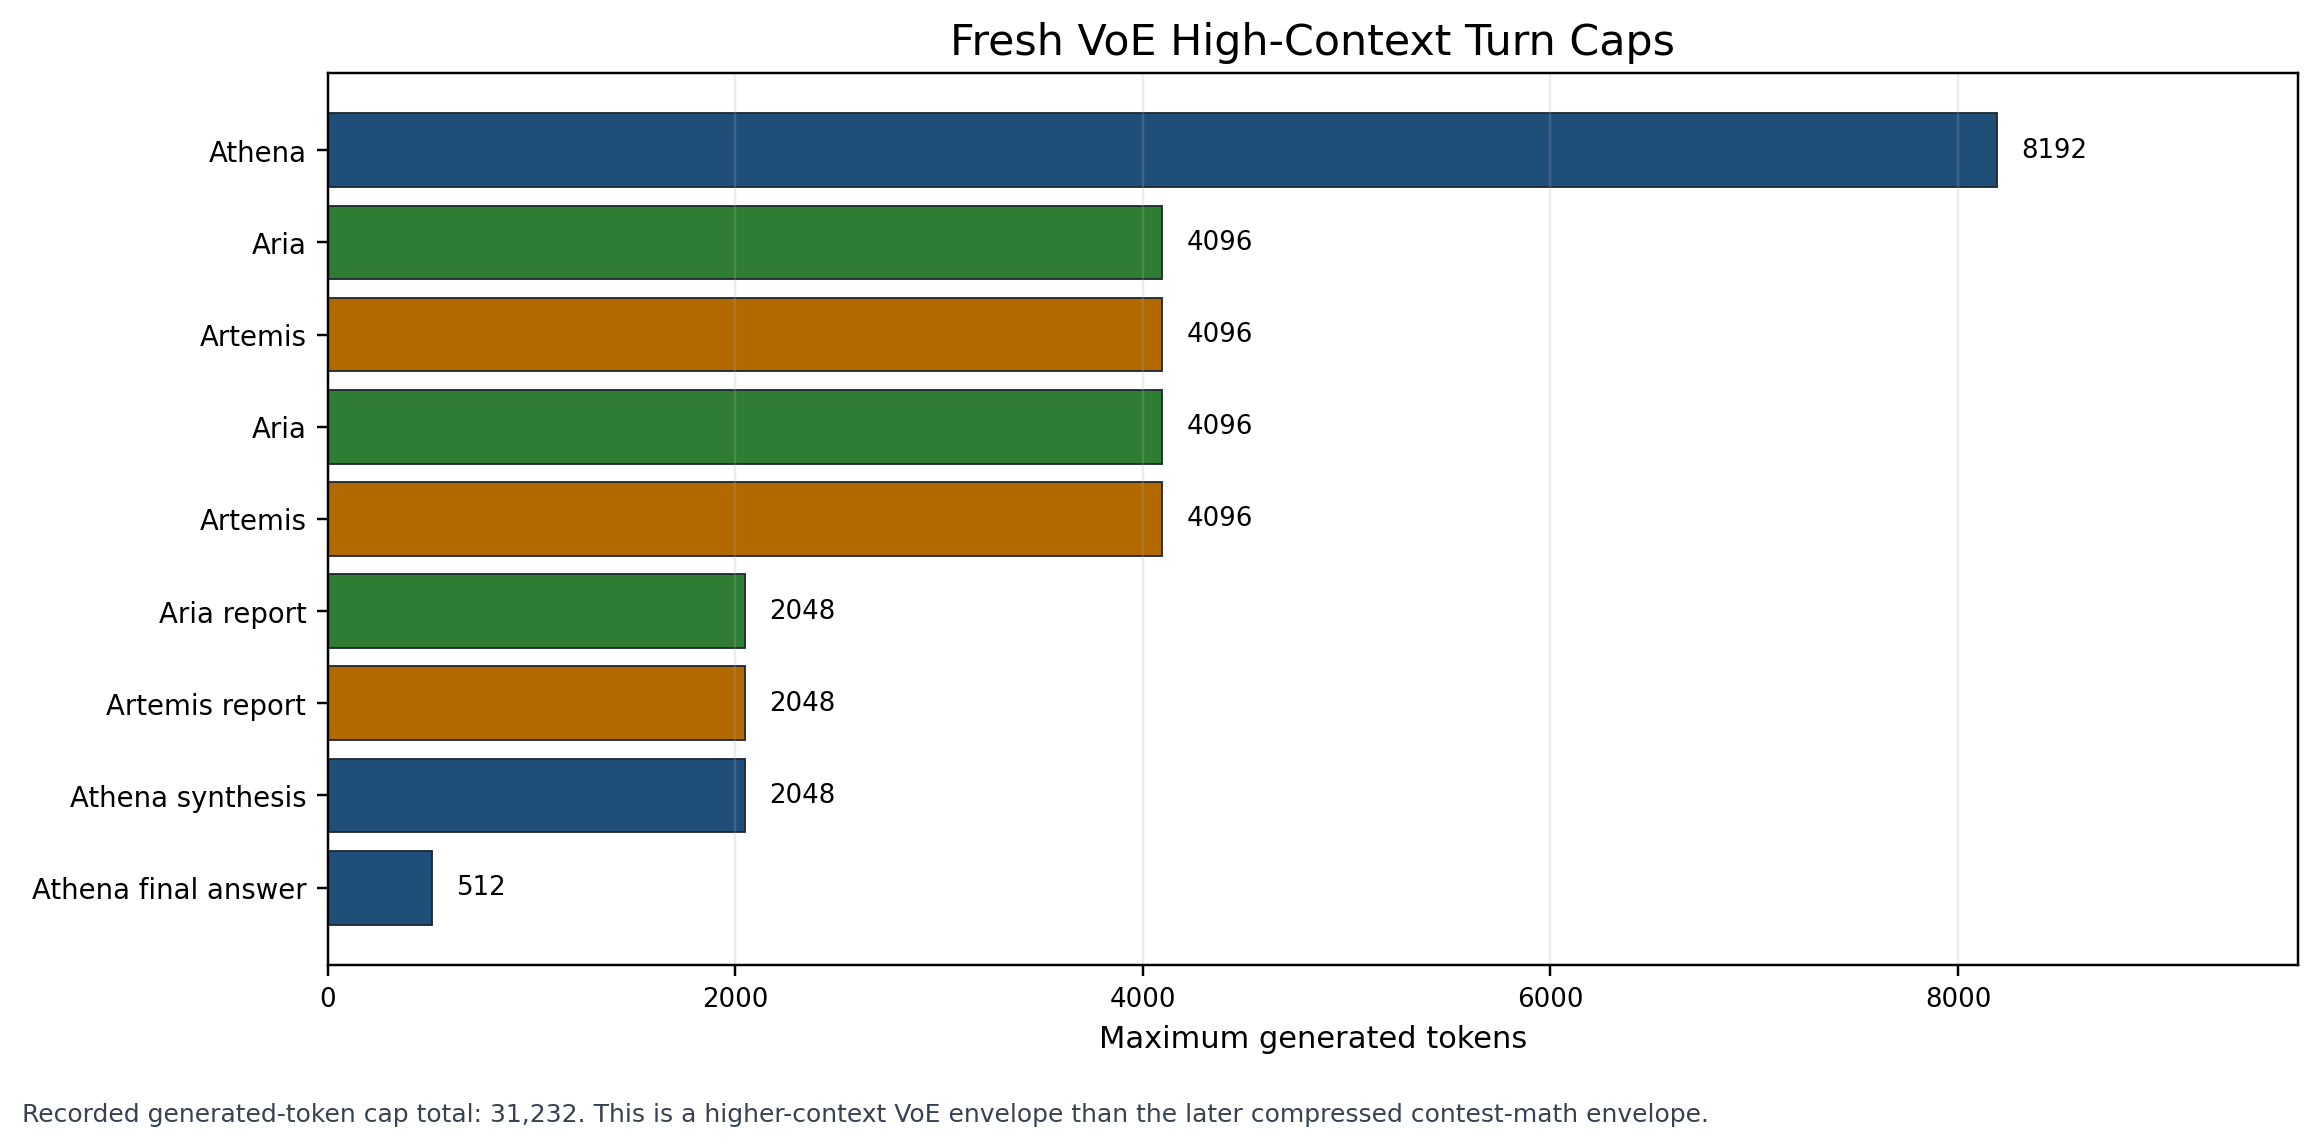
\includegraphics[width=\linewidth]{diagrams/voe_high_context_token_caps.png}
\caption{Fresh VoE high-context generated-token caps. The recorded VoE schema is materially larger than the later compressed contest-math schema, so the two diagnostics should not be interpreted as sharing the same token budget.}
\label{fig:voe-high-context-token-caps}
\end{figure}

\subsection{Memory-Loaded Vault of Echoes Run (Certified Recall)}

The memory-loaded VoE condition asks a different question. Instead of testing the fresh no-answer-memory path, it loads answer-bearing golden prompt rows for the ten cases missed by the fresh run using the version 18 Runtime-at-Boot memory surface, then requires the role sessions to pass certification before solve-time replay. Under the same 25-case VoE surface and the same high-context controller shape, the memory-certified condition recovers the ten missed cases, giving 25/25.

This result is reported as a certified-memory result, not as an ordinary no-memory benchmark score. Its purpose is to show the effect of active prompt memory when the controller verifies that the relevant golden rows were read before inference. The fresh run gives the no-answer-memory baseline at 15/25; the memory-loaded replay shows that certified answer-bearing memory can convert the same VoE surface to 25/25 under the recorded runtime discipline.

\begin{figure}[H]
\centering
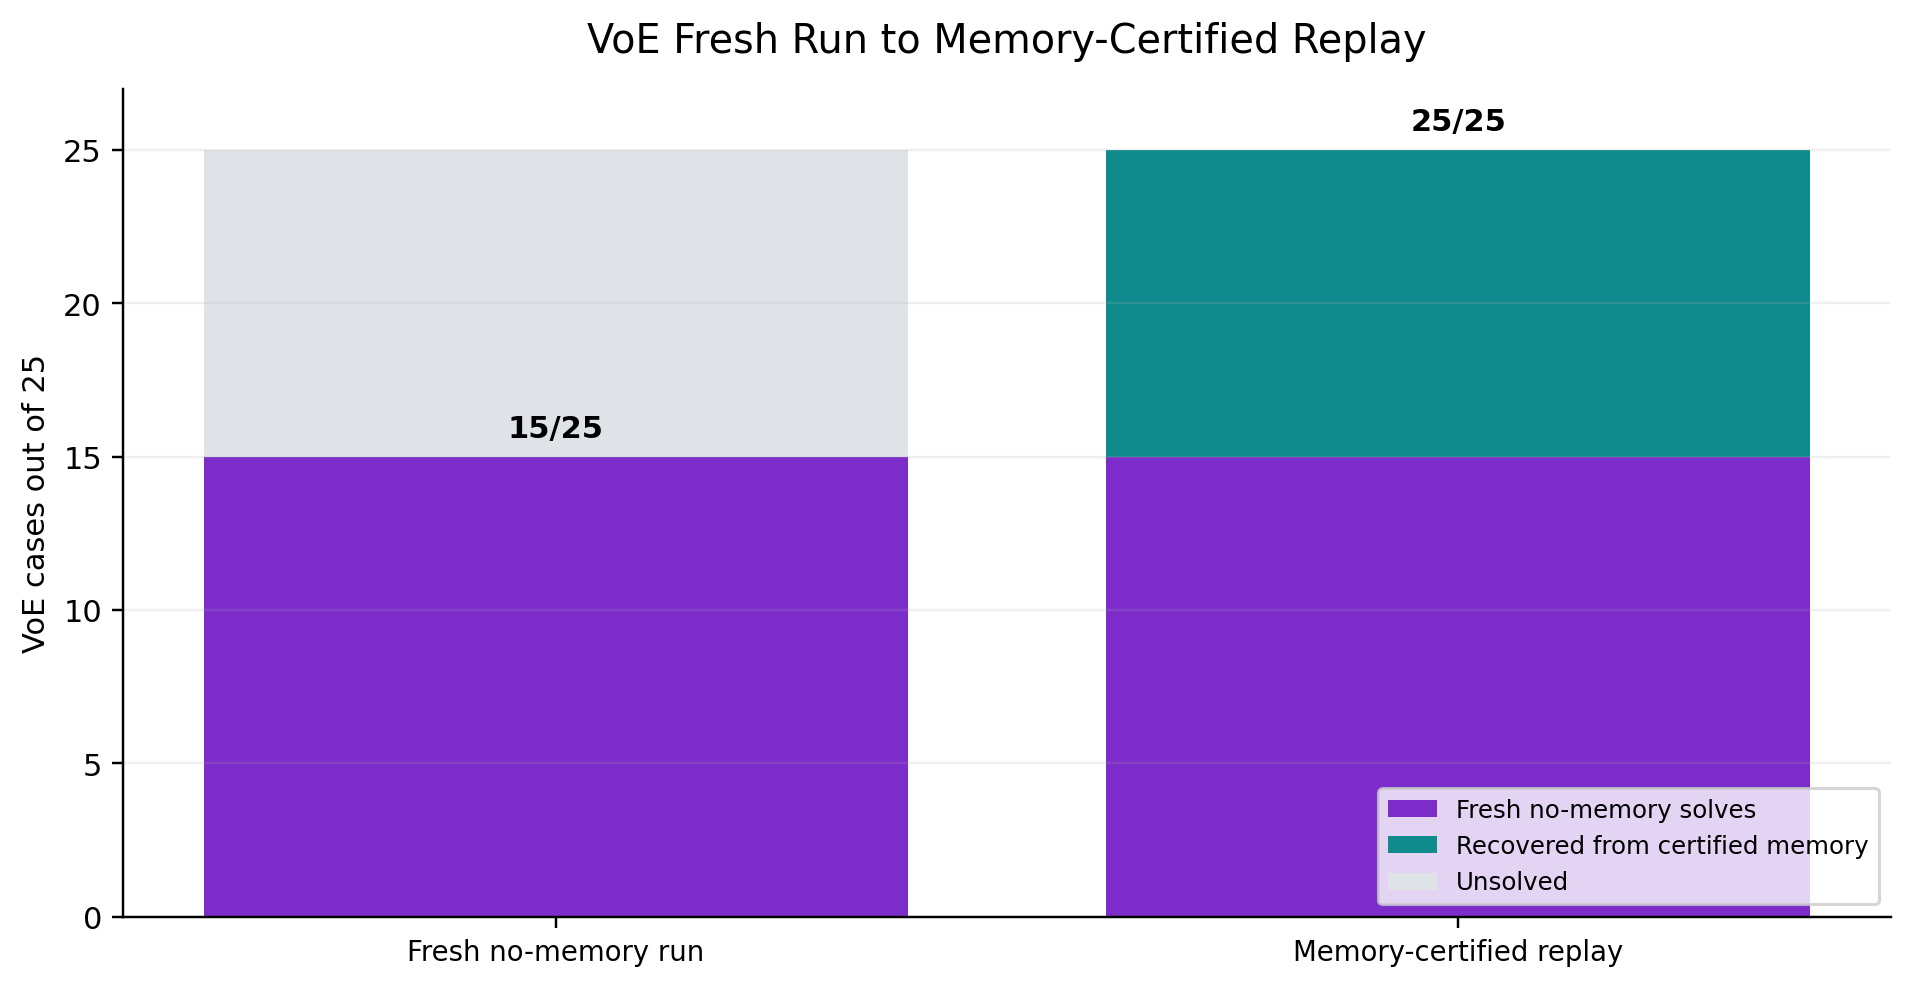
\includegraphics[width=\linewidth]{diagrams/voe_memory_lift.png}
\caption{VoE fresh run to memory-certified replay. The fresh no-answer-memory run solves 15/25; the version 18 memory-loaded condition supplies certified golden rows for the ten missed cases and recovers the full 25/25 surface.}
\label{fig:voe-memory-lift}
\end{figure}

\paragraph{Results analysis.}
These two VoE runs prove a bounded internal effect for \rab{}: on the same 25-case surface, the fresh no-answer-memory condition scores 15/25, while the memory-certified condition scores 25/25 after the exact canonical solution rows for the ten missed cases are supplied and certified. It is direct evidence that certified prompt memory can change the controller-selected answer on this internal benchmark. A useful transcript-level example is p08, ``Two Clues, One Suspect.'' In the fresh condition, AEN does not close the problem; in the memory-certified replay, the correct value is supplied to the controller after the relevant certified row is available. The transcript does not show a stable independent derivation emerging from scratch. It instead shows the answer-bearing memory becoming active enough to affect finalization, which is precisely the \rab{} effect being isolated here.

A natural future comparison is low-data supervised fine-tuning: we hypothesize that training on only the ten missed solution rows, even with repeated epochs, would not reliably reproduce this behavior without overfitting or harming adjacent behavior. That experiment is not performed here, so the supervised-fine-tuning comparison remains a hypothesis rather than a result.

\subsection{American Invitational Mathematics Examination (AIME) 2026 frozen-notebook diagnostic}

The resource conclusion from VoE motivated the AIME diagnostic. The fresh VoE Kaggle workflow required 12336.25 seconds for 25 problems, about 3.43 hours, before considering the larger target of 50 competition-style problems. That envelope is too expensive for constrained settings such as an AIMO-style five-hour graphics-processing-unit runtime. The contest-math notebook was therefore compressed aggressively: Athena opening was capped at 1024 generated tokens, peer exchanges and peer reports at 1280, Athena synthesis at 768, and final emission at 128. The run used a G4-class graphics-processing-unit runtime with 96 GB of memory, not an H100 runtime. Because public AIMO test rows were not available, the compressed exact-integer diagnostic was run on an AIME-style surface instead.

The held-out contest-math diagnostic used an AIME 2026 test comma-separated values file converted from a local parquet copy and executed through the same frozen one-loop notebook path. The export bundle contains \path{score_summary.json}, \path{scored_results.csv}, \path{attached_test_full_log.csv}, per-problem \path{result_payloads/}, per-problem transcripts, the runtime boot log, and a short analysis note. The run records 30 cases, \path{runtime_at_boot_passed: true}, total wall time 5489.579 seconds, and exact-answer accuracy 15/30 \((50.0\%)\). The evidence below is derived from those files rather than from a manual score table.

\begin{table}[H]
\centering
\small
\begin{tabularx}{\linewidth}{p{0.30\linewidth}X}
\toprule
Measured field & Observed value \\
\midrule
Cases & 30 \\
Exact-answer correctness & 15/30 \((50.0\%)\) \\
\rab{} status & Passed \\
Runtime hardware & G4-class graphics-processing-unit runtime; 96 GB memory; not H100 \\
Wall time & 5489.579 seconds \((\approx 91.5\) minutes) \\
Mean wall time/problem & 182.98 seconds \((\approx 3.05\) minutes) \\
Mean total tokens/problem & 711,100 \\
Mean completion tokens/problem & 7,767 \\
Controller shape & 1 loop; 9 role turns per problem \\
Problems 1--8 & 8/8 exact matches \\
Problems 9--15 & 0/7 exact matches \\
Problems 16--22 & 4/7 exact matches \\
Problems 23--30 & 3/8 exact matches \\
Exact-consensus closeouts & 14 correct, 2 incorrect \\
Majority-vote fallback closeouts & 1 correct, 6 incorrect \\
Highest-confidence fallback closeouts & 0 correct, 7 incorrect \\
Athena opening cap hits & 29/30 at 1024 generated tokens \\
Athena synthesis cap hits & 22/30 at 768 generated tokens \\
Peer turn cap & 1280 generated tokens for exchanges and reports \\
\bottomrule
\end{tabularx}
\caption{American Invitational Mathematics Examination (AIME) 2026 frozen-notebook diagnostic. This reports the constrained one-loop notebook rather than the architecture's larger-resource ceiling.}
\label{tab:aime2026-frozen}
\end{table}

Figure~\ref{fig:aime2026-frozen-problem-outcomes} shows the outcome matrix by problem index. Each cell records the emitted answer; missed cells also show the expected answer. The first eight problems close cleanly, the 9--15 band collapses, and the later bands recover only partially. The diagnostic is therefore not a uniform random failure pattern; it is a compressed-budget run whose reliability changes sharply as problem difficulty and route length increase.

\begin{figure}[H]
\centering
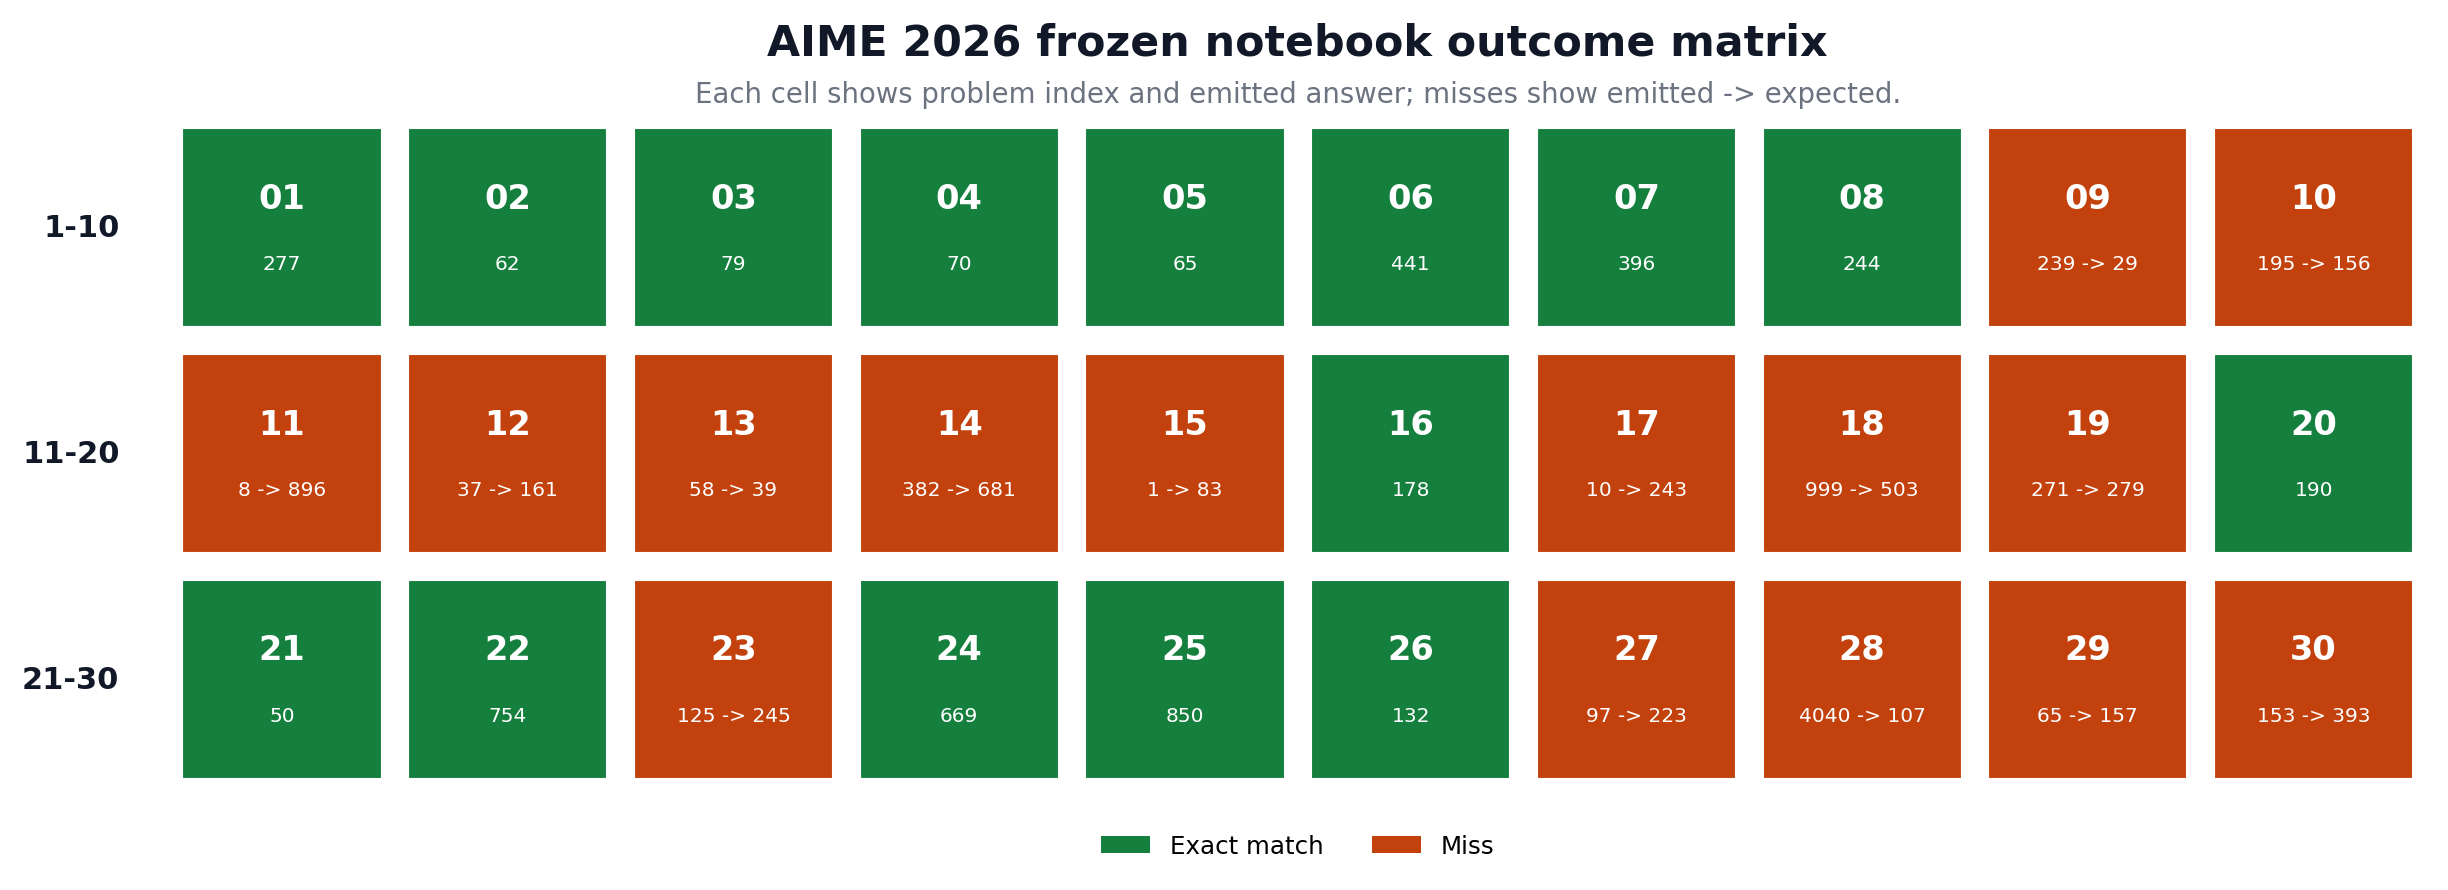
\includegraphics[width=\linewidth]{diagrams/aime2026_frozen_problem_outcomes.png}
\caption{AIME 2026 frozen-notebook exact-match outcome matrix. Green cells are exact matches; red cells are misses and show emitted answer \(\rightarrow\) expected answer.}
\label{fig:aime2026-frozen-problem-outcomes}
\end{figure}

The closeout modes are the strongest calibration signal. Figure~\ref{fig:aime2026-frozen-closeout-calibration} shows that strict three-role consensus is usually reliable under this envelope, but fallbacks are not: strict consensus closes 14/16 correctly, majority vote closes 1/7 correctly, and highest-confidence fallback closes 0/7 correctly. The controller's \path{verified=true} field is therefore a structural closeout record. It should not be read as mathematical correctness without the external answer key.

\begin{figure}[H]
\centering
\begin{minipage}{0.54\linewidth}
\centering
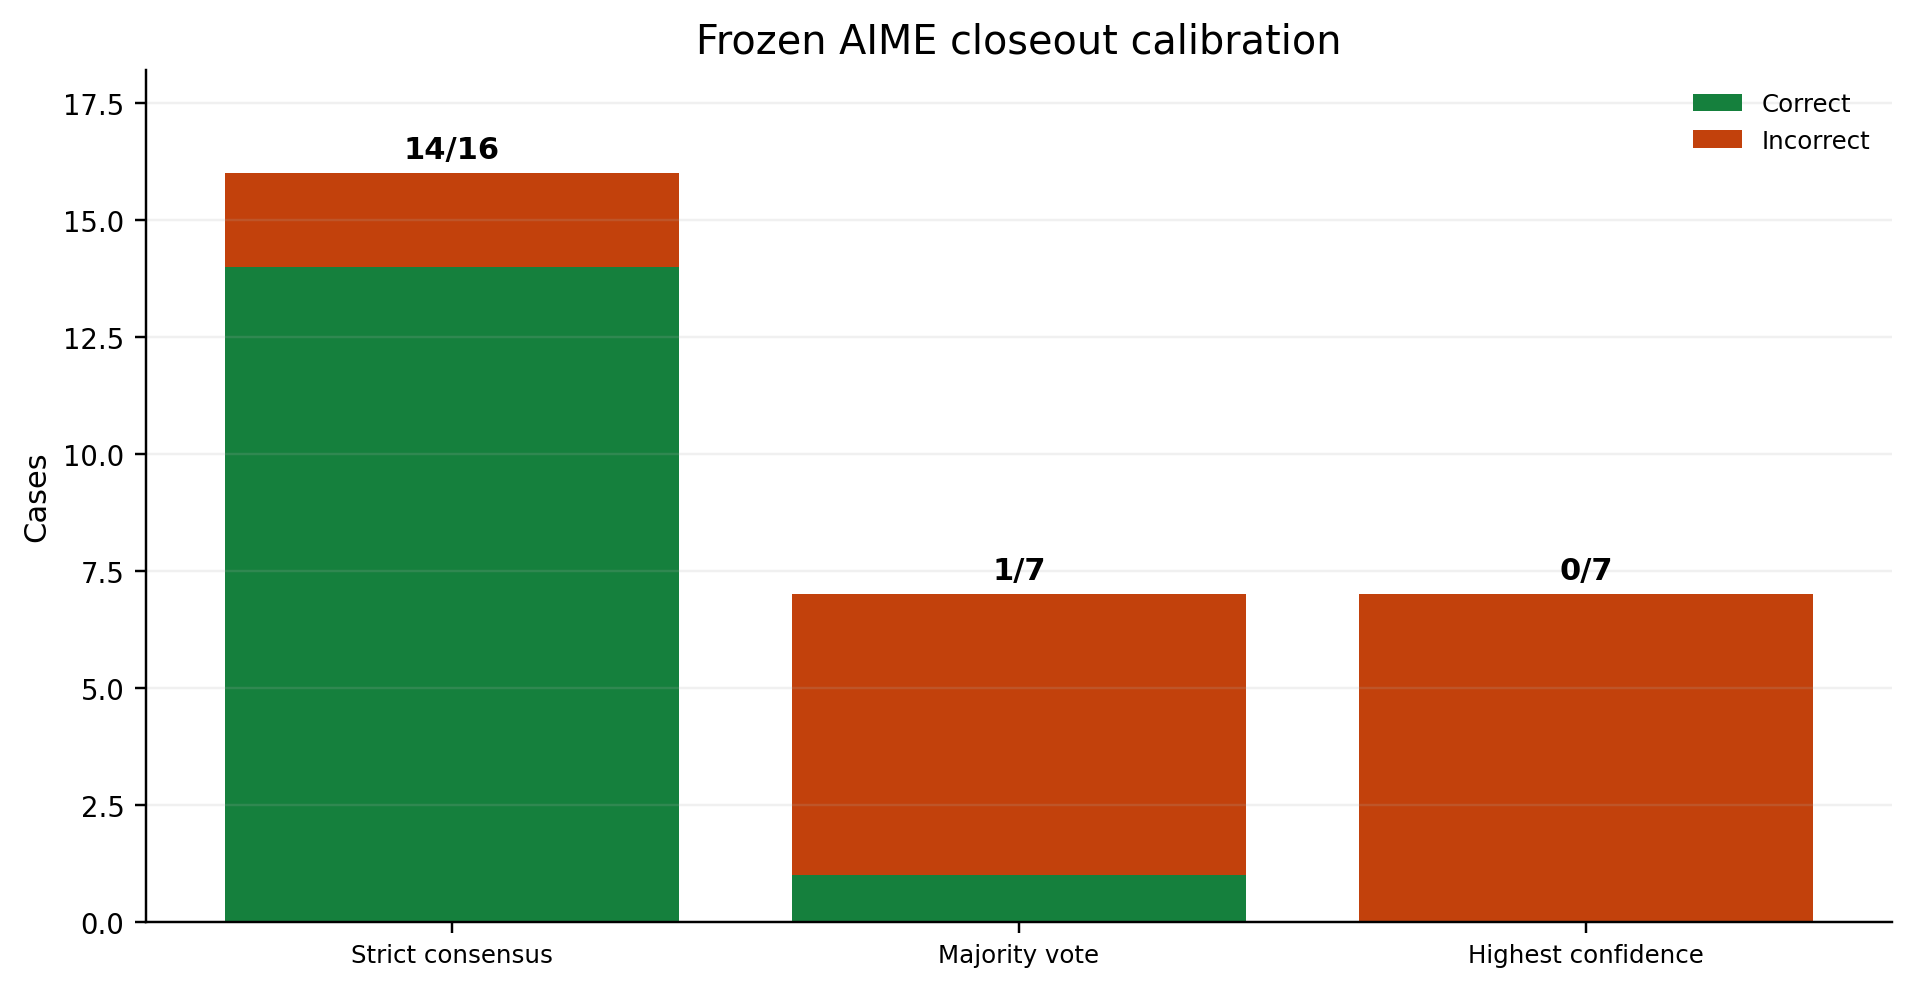
\includegraphics[width=\linewidth]{diagrams/aime2026_frozen_closeout_calibration.png}
\end{minipage}
\hfill
\begin{minipage}{0.42\linewidth}
\centering
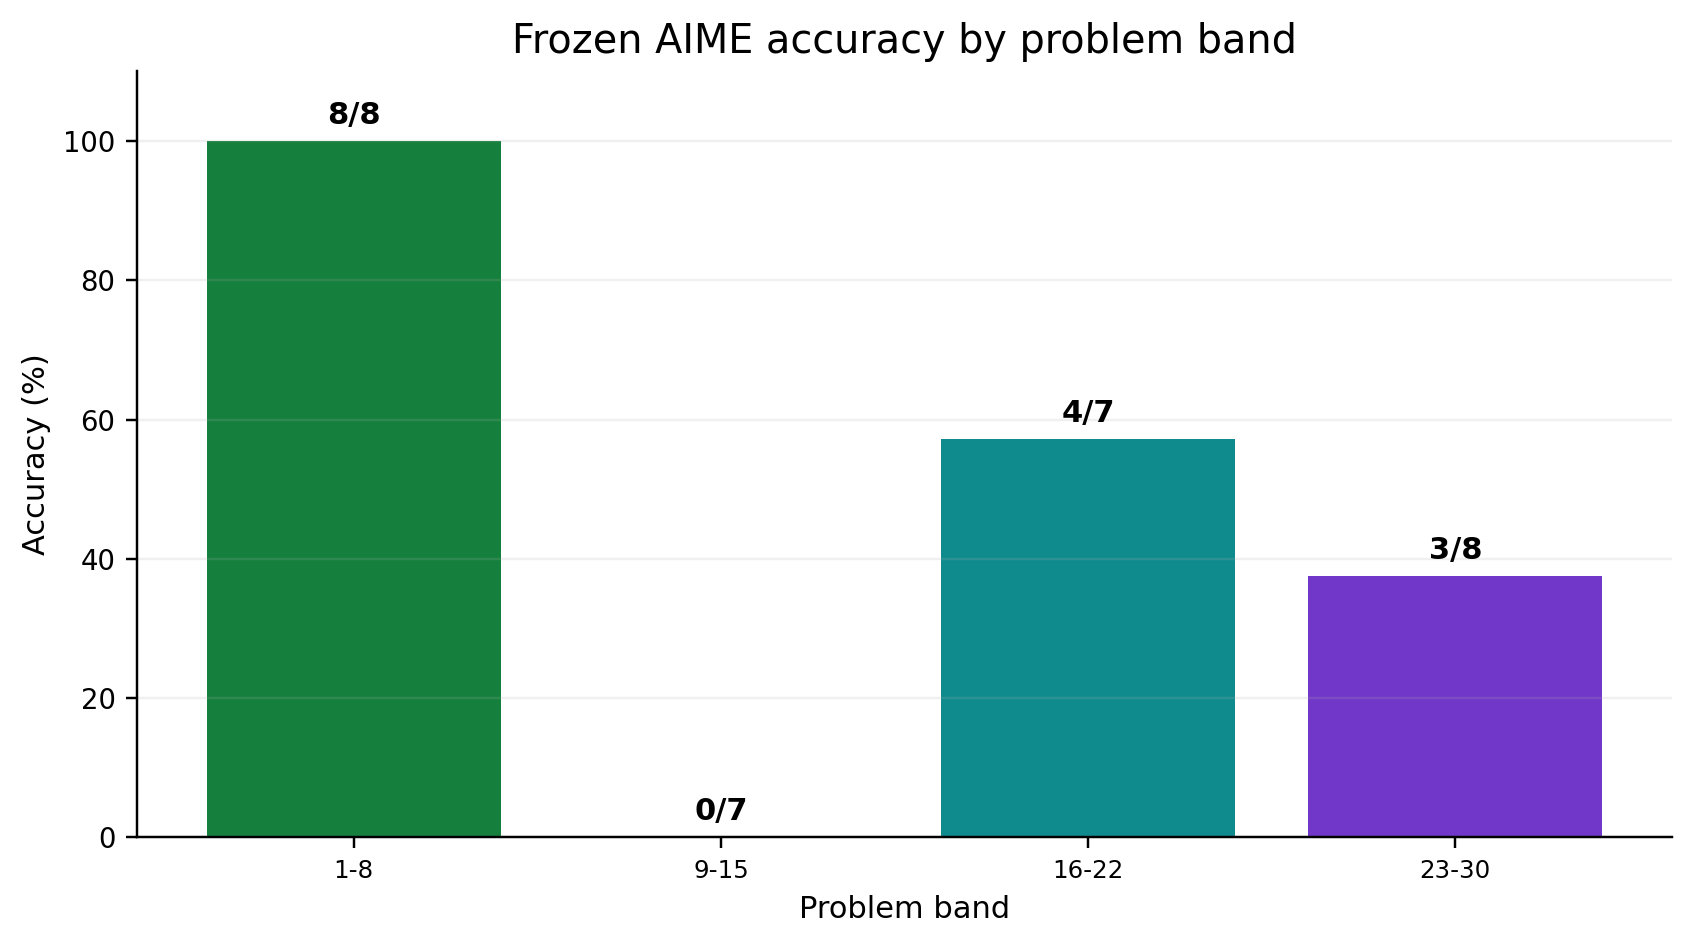
\includegraphics[width=\linewidth]{diagrams/aime2026_frozen_band_accuracy.png}
\end{minipage}
\caption{AIME 2026 closeout calibration and problem-band accuracy. Consensus is the reliable mode in this run; fallback modes are weak under the compressed envelope.}
\label{fig:aime2026-frozen-closeout-calibration}
\end{figure}

The token evidence explains why the run should be read as context-pruned. Figure~\ref{fig:aime2026-frozen-token-cap-pressure} reports generated-token cap hits by controller phase. Athena's opening turn hit its 1024-token cap in 29/30 cases, and Athena synthesis hit its 768-token cap in 22/30 cases. Peer turns also show substantial cap pressure: Aria exchange 1 hit 22/30, Artemis exchange 1 hit 16/30, Aria exchange 2 hit 17/30, and Artemis exchange 2 hit 14/30. In other words, the run is not merely a weaker mathematical attempt; it is a deliberately compressed controller execution.

\begin{figure}[H]
\centering
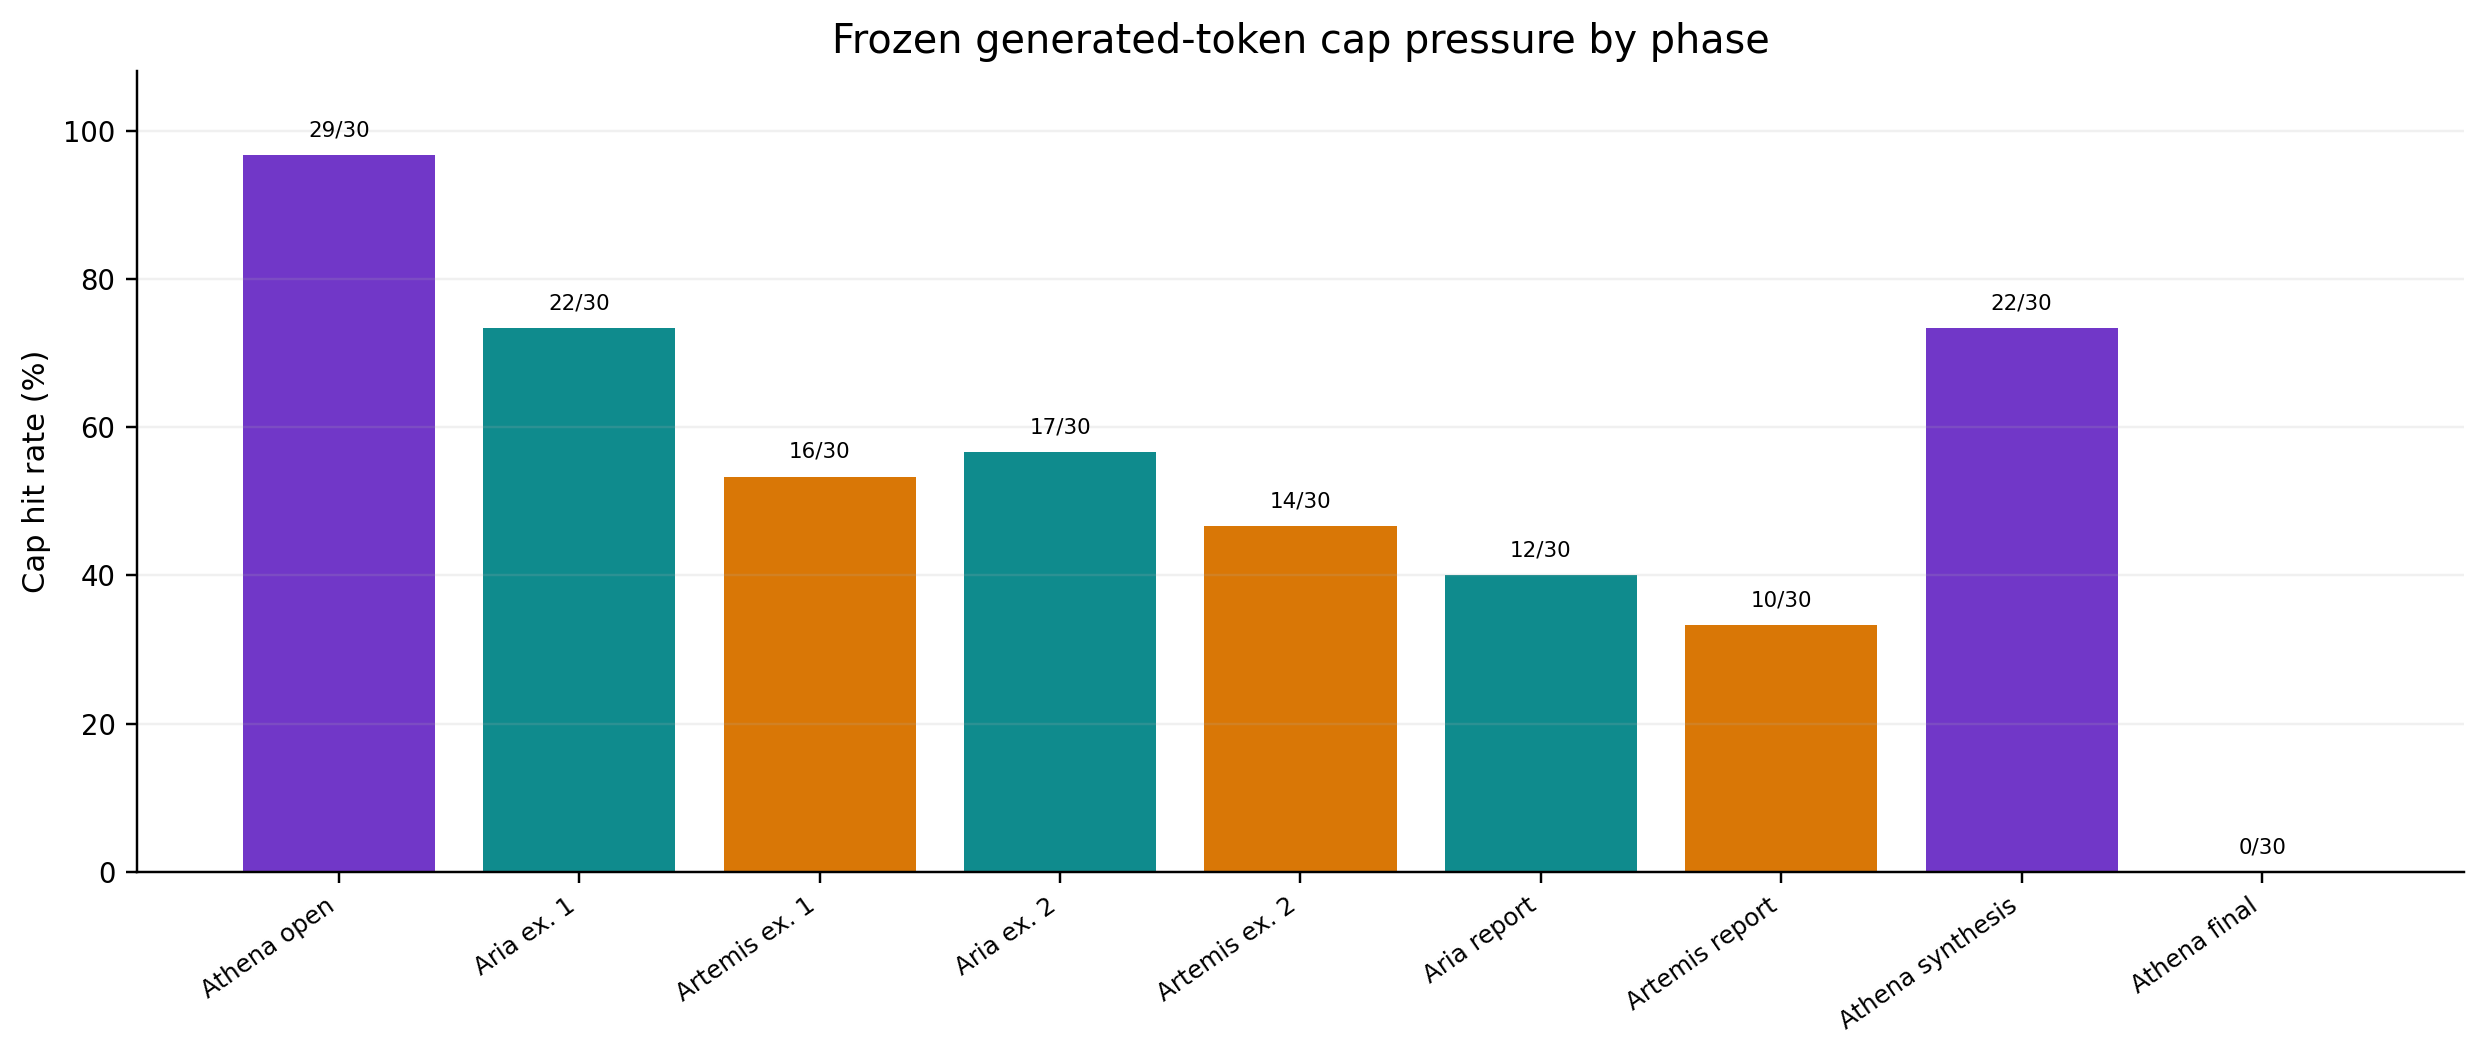
\includegraphics[width=\linewidth]{diagrams/aime2026_frozen_token_cap_pressure.png}
\caption{Generated-token cap pressure by controller phase in the AIME 2026 frozen notebook. Each label gives cap hits out of 30 turns for that phase.}
\label{fig:aime2026-frozen-token-cap-pressure}
\end{figure}

Figure~\ref{fig:aime2026-frozen-runtime-tokens} pairs wall time with generated-token load. The average case uses about 7,767 completion tokens and 711,100 total tokens after long-context prompt memory is included. Misses cluster among longer, cap-heavy cases, but runtime alone is not sufficient to predict correctness: the decisive variable is whether the constrained turns close the mathematical route before synthesis and finalization.

\begin{figure}[H]
\centering
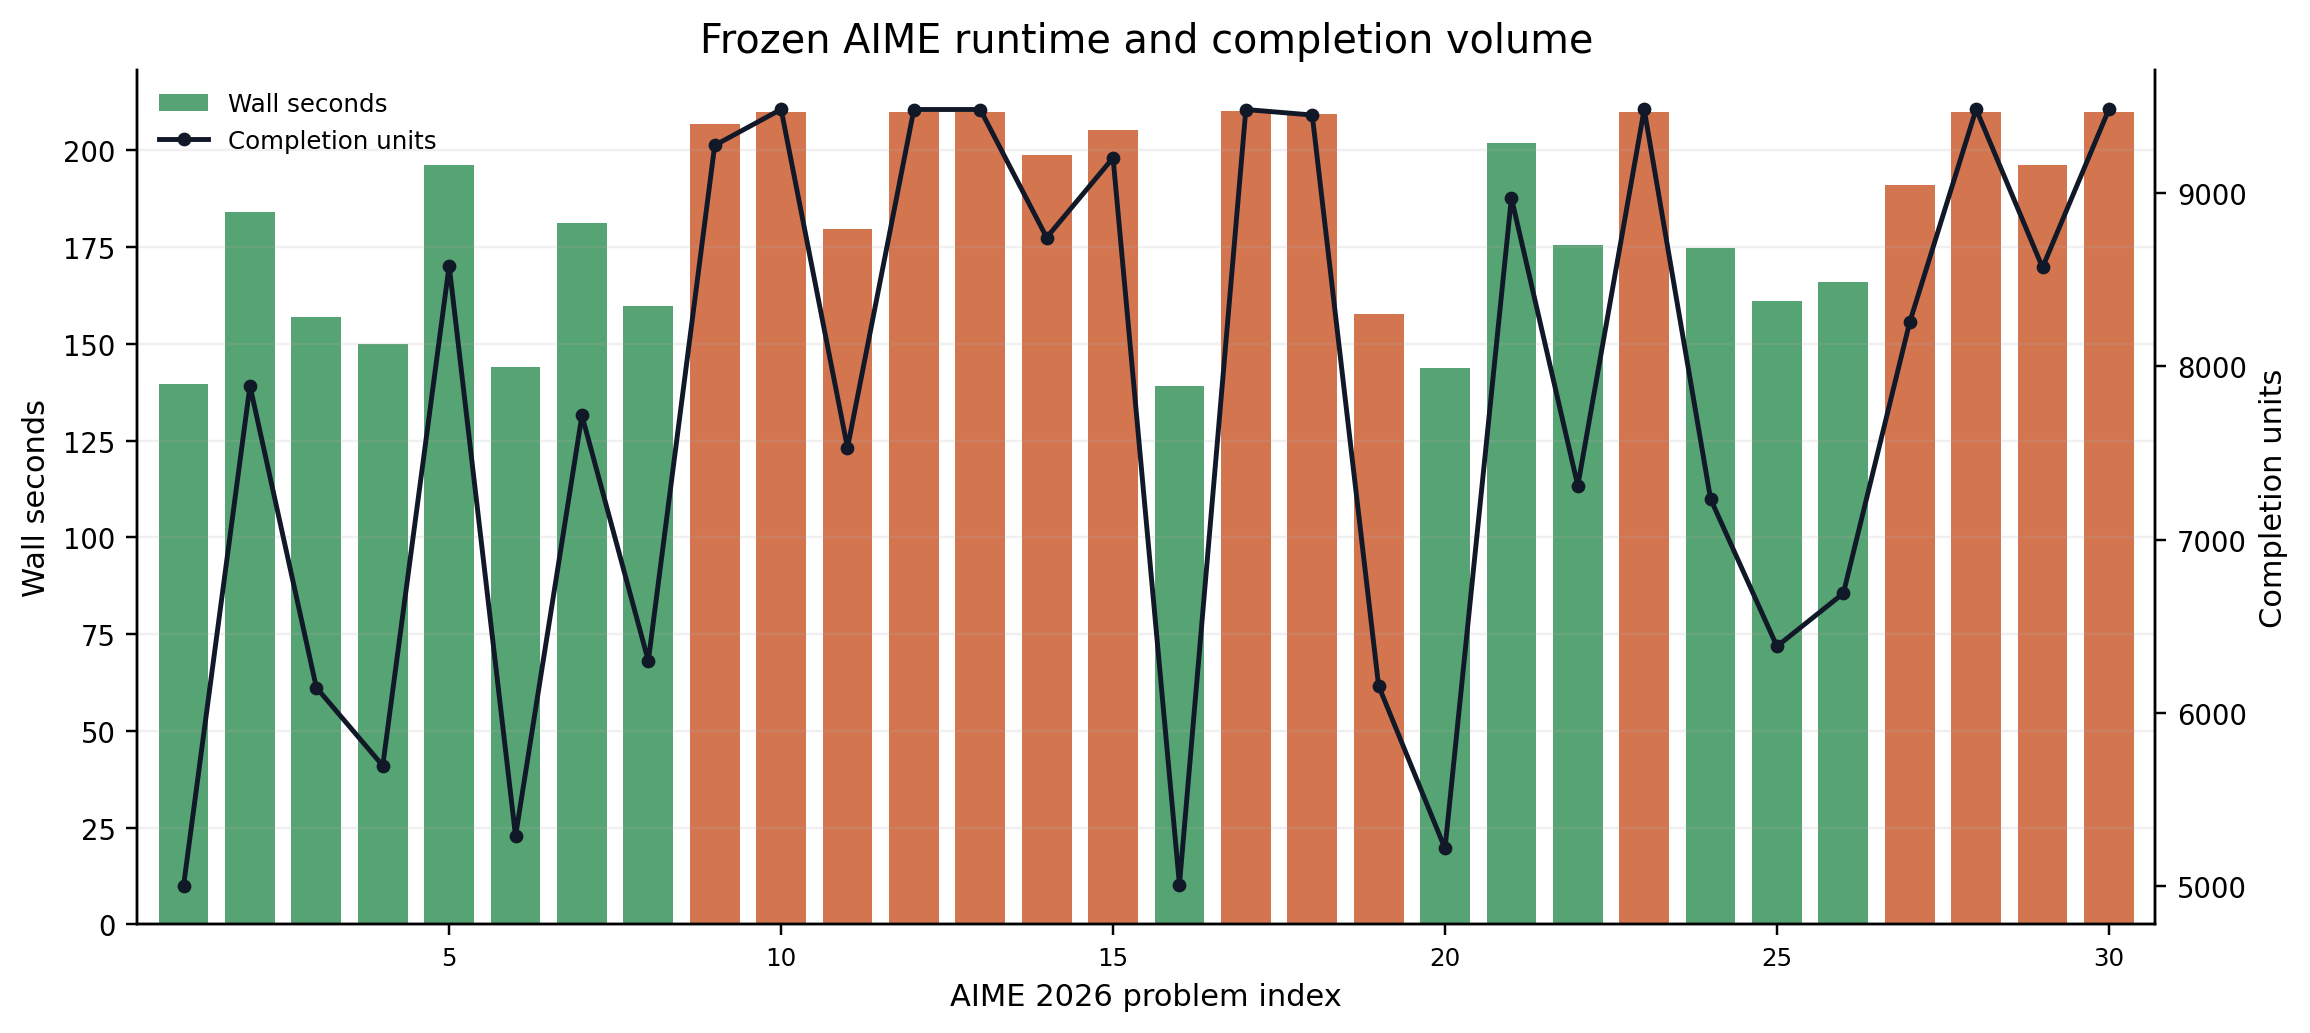
\includegraphics[width=\linewidth]{diagrams/aime2026_frozen_runtime_tokens.png}
\caption{AIME 2026 runtime and generated-token load by problem. Bars show wall seconds, while the line shows completion tokens; green bars are exact matches and red bars are misses.}
\label{fig:aime2026-frozen-runtime-tokens}
\end{figure}

The transcript-level failure examples support the same interpretation. The analysis note flags \path{aime2026_11}, where strict consensus emits \(8\) instead of \(896\); \path{aime2026_27}, where strict consensus emits \(97\) instead of \(223\); \path{aime2026_28}, where highest-confidence fallback emits \(4040\) instead of \(107\); and \path{aime2026_30}, where synthesis is visibly mid-enumeration when the final answer is emitted. These are not only answer-normalization failures. They are route-completion and fallback-calibration failures under a deliberately pruned one-loop budget.

Because the AIME diagnostic has exactly 30 problems, percentage claims have coarse granularity. The only possible exact scores near the high-accuracy regime are 27/30 \(=90.0\%\), 28/30 \(\approx 93.3\%\), 29/30 \(\approx 96.7\%\), and 30/30 \(=100.0\%\). Thus any future claim of ``95\%+'' performance on this slice must mean at least 29 correct answers, and intermediate percentages such as 92\% should not be reported for a 30-case AIME run.

\subsection{Unrestricted One-Loop AIME 2026 Run}

The next AIME run used the Hugging Face \path{MathArena/aime_2026} source and the export directory \path{aime2026_hf_full_export_20260422-161358}. This run is called unrestricted relative to the frozen notebook because the per-turn generation caps were expanded and a third peer exchange was enabled. It was still a one-loop run: the controller used 11 role turns per problem, not a multi-loop search. The export records both token-accounting fields and transcript character volume, so this section reports accuracy, controller mode, generated completion volume, wall time, and character-scale transcript growth together.

\begin{table}[H]
\centering
\small
\begin{tabularx}{\linewidth}{p{0.30\linewidth}X}
\toprule
Measured field & Observed value \\
\midrule
Dataset source & \path{MathArena/aime_2026} \\
Cases & 30 \\
Exact-answer correctness & 22/30 \((73.33\%)\) \\
\rab{} status & Passed \\
Controller shape & 1 loop; 11 role turns per problem; 3 peer exchanges \\
Wall time & 11411.925 seconds \((\approx 190.2\) minutes) \\
Mean wall time/problem & 380.39 seconds \((\approx 6.34\) minutes) \\
Mean total tokens/problem & 1,125,451 \\
Mean completion units/problem & 16,972 \\
Mean transcript characters/problem & 45,143 \\
Problems 1--8 & 8/8 exact matches \\
Problems 9--15 & 2/7 exact matches \\
Problems 16--22 & 6/7 exact matches \\
Problems 23--30 & 6/8 exact matches \\
Strict-consensus closeouts & 14 correct, 2 incorrect \\
Majority-vote fallback closeouts & 8 correct, 5 incorrect \\
Highest-confidence fallback closeouts & 0 correct, 1 incorrect \\
\bottomrule
\end{tabularx}
\caption{Unrestricted one-loop AIME 2026 run. The run expands generation room and peer exchange count while keeping the controller to one loop.}
\label{tab:aime2026-unrestricted}
\end{table}

Figure~\ref{fig:aime2026-unrestricted-outcomes} shows the unrestricted outcome matrix. The early band remains clean, and the larger budget recovers several mid- and late-band failures that the frozen run missed. The missed set shrinks to eight problems: 9, 10, 13, 14, 15, 18, 29, and 30.

\begin{figure}[H]
\centering
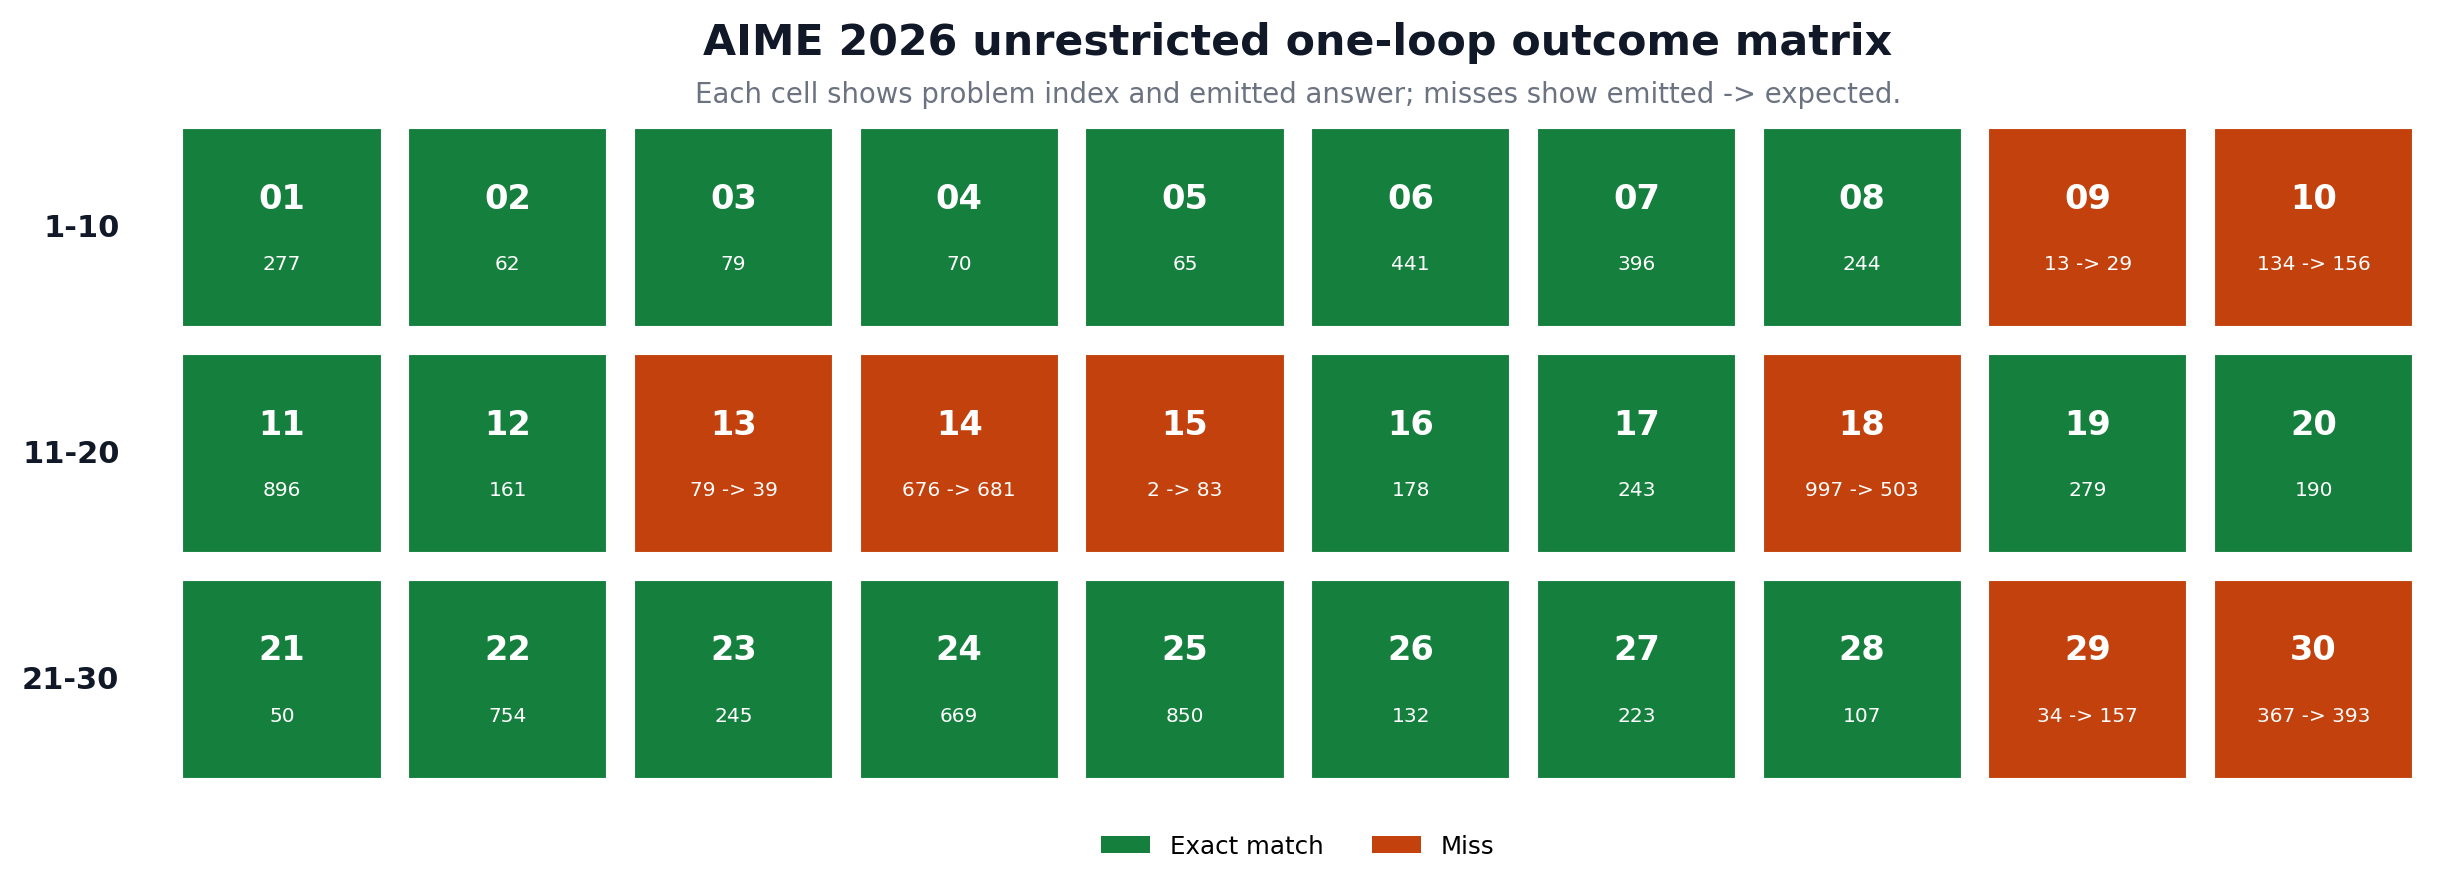
\includegraphics[width=\linewidth]{diagrams/aime2026_unrestricted_problem_outcomes.png}
\caption{Unrestricted one-loop AIME 2026 outcome matrix. Green cells are exact matches; red cells are misses and show emitted answer \(\rightarrow\) expected answer.}
\label{fig:aime2026-unrestricted-outcomes}
\end{figure}

Figure~\ref{fig:aime2026-unrestricted-calibration} shows that expanded budget mainly improves fallback usefulness. Strict consensus remains 14/16, but majority fallback improves from a weak mode in the frozen run to 8/13 in the unrestricted run. This suggests that the additional peer exchange and larger generation budget made non-consensus states more informative without changing the final controller loop count.

\begin{figure}[H]
\centering
\begin{minipage}{0.54\linewidth}
\centering
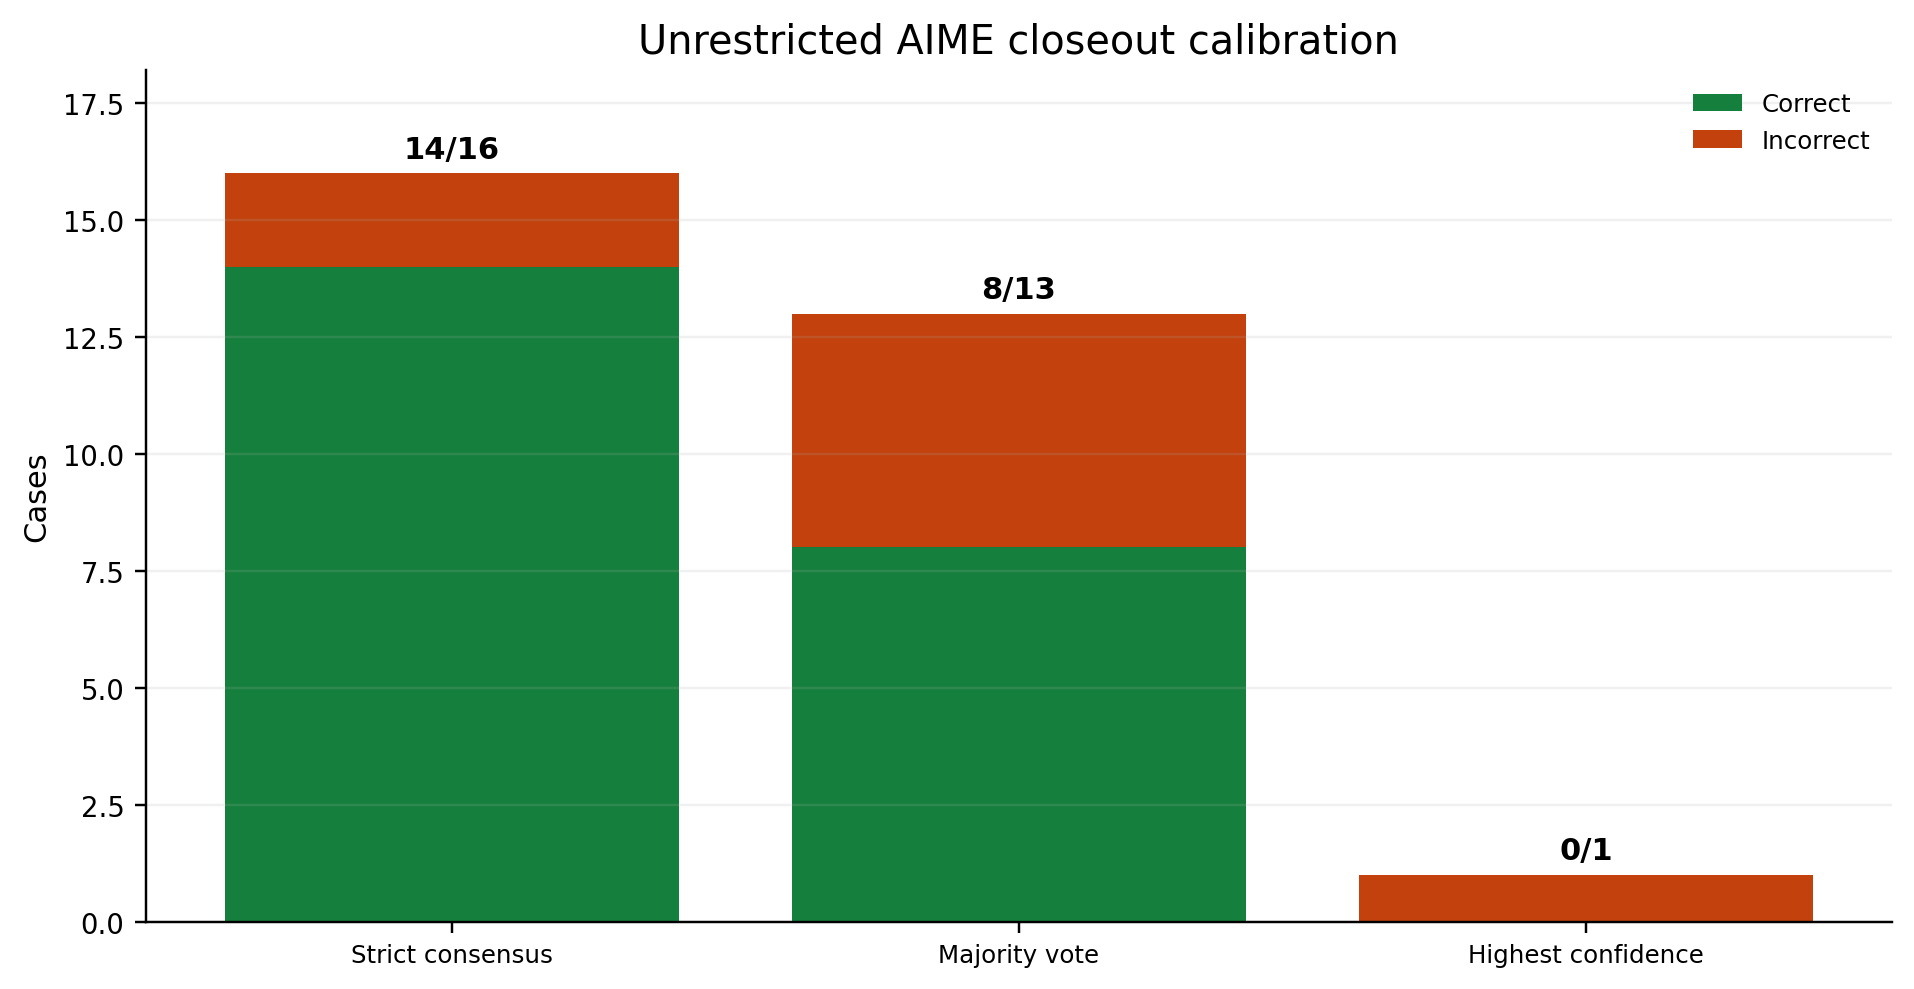
\includegraphics[width=\linewidth]{diagrams/aime2026_unrestricted_closeout_calibration.png}
\end{minipage}
\hfill
\begin{minipage}{0.42\linewidth}
\centering
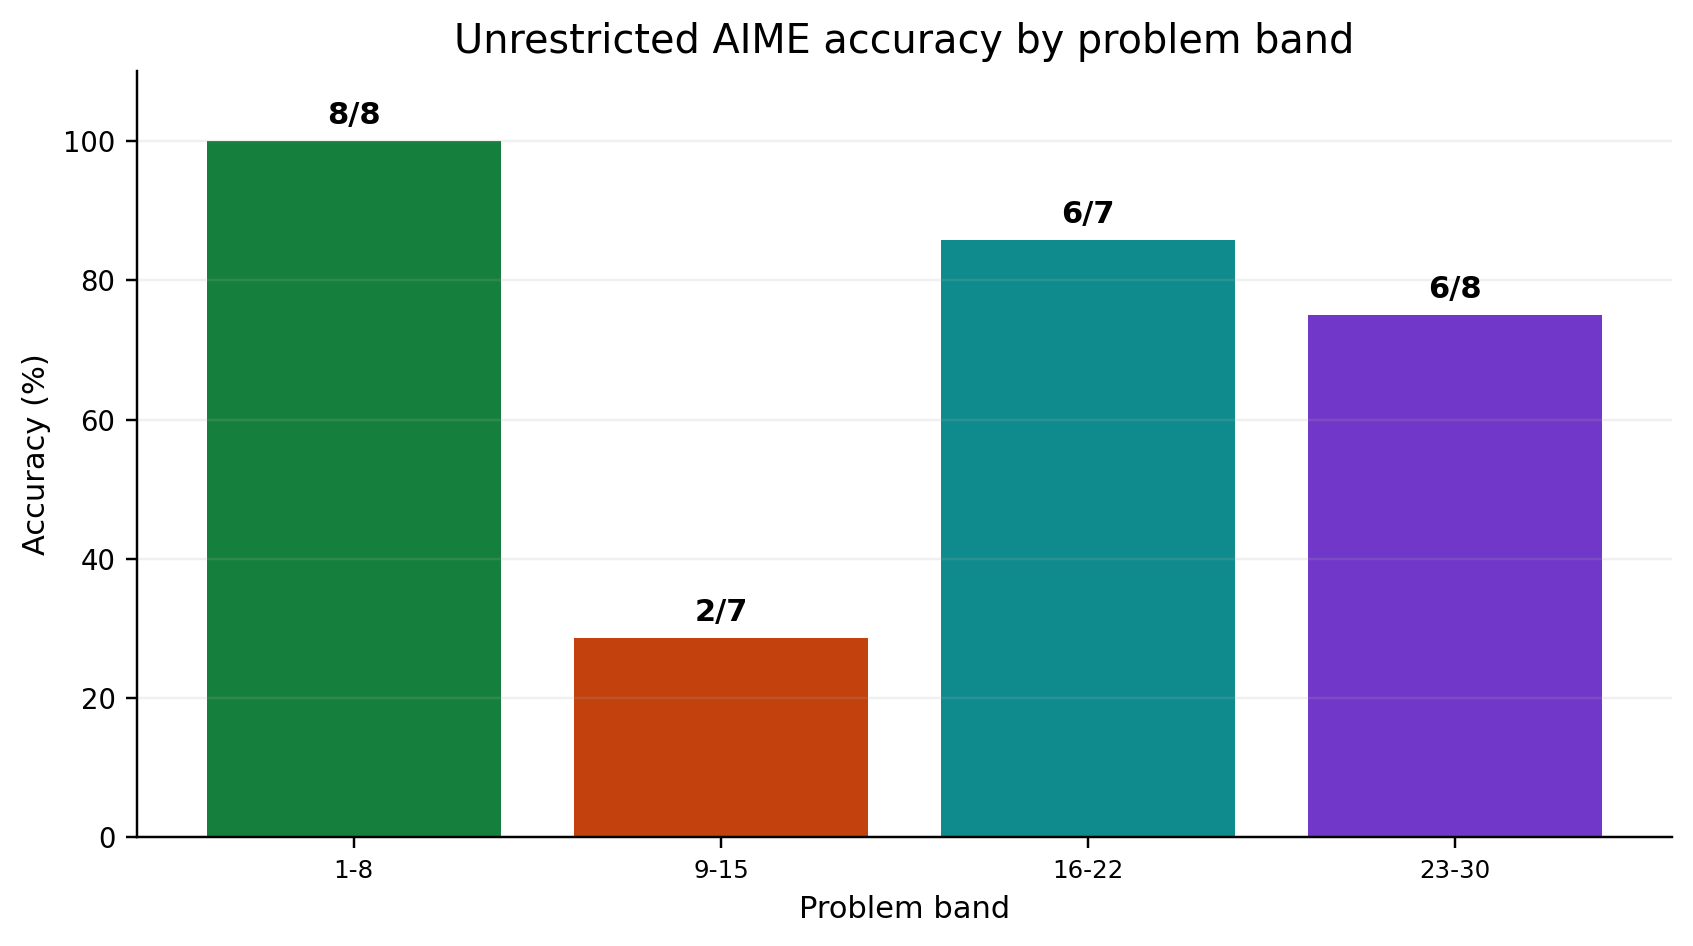
\includegraphics[width=\linewidth]{diagrams/aime2026_unrestricted_band_accuracy.png}
\end{minipage}
\caption{Unrestricted AIME closeout calibration and problem-band accuracy. The larger one-loop run improves the middle and late bands while preserving the clean early band.}
\label{fig:aime2026-unrestricted-calibration}
\end{figure}

The unrestricted run is not free. Figure~\ref{fig:aime2026-unrestricted-cap-pressure} shows that the expanded 4096-unit phases are still sometimes saturated, especially Athena open and first peer exchanges. Figure~\ref{fig:aime2026-unrestricted-runtime-volume} shows the corresponding wall-time and transcript-character growth. The run improves accuracy by giving the roles more room to develop routes, but the recorded transcript sizes show why this setting is not a drop-in replacement for a tightly constrained competition runtime.

\begin{figure}[H]
\centering
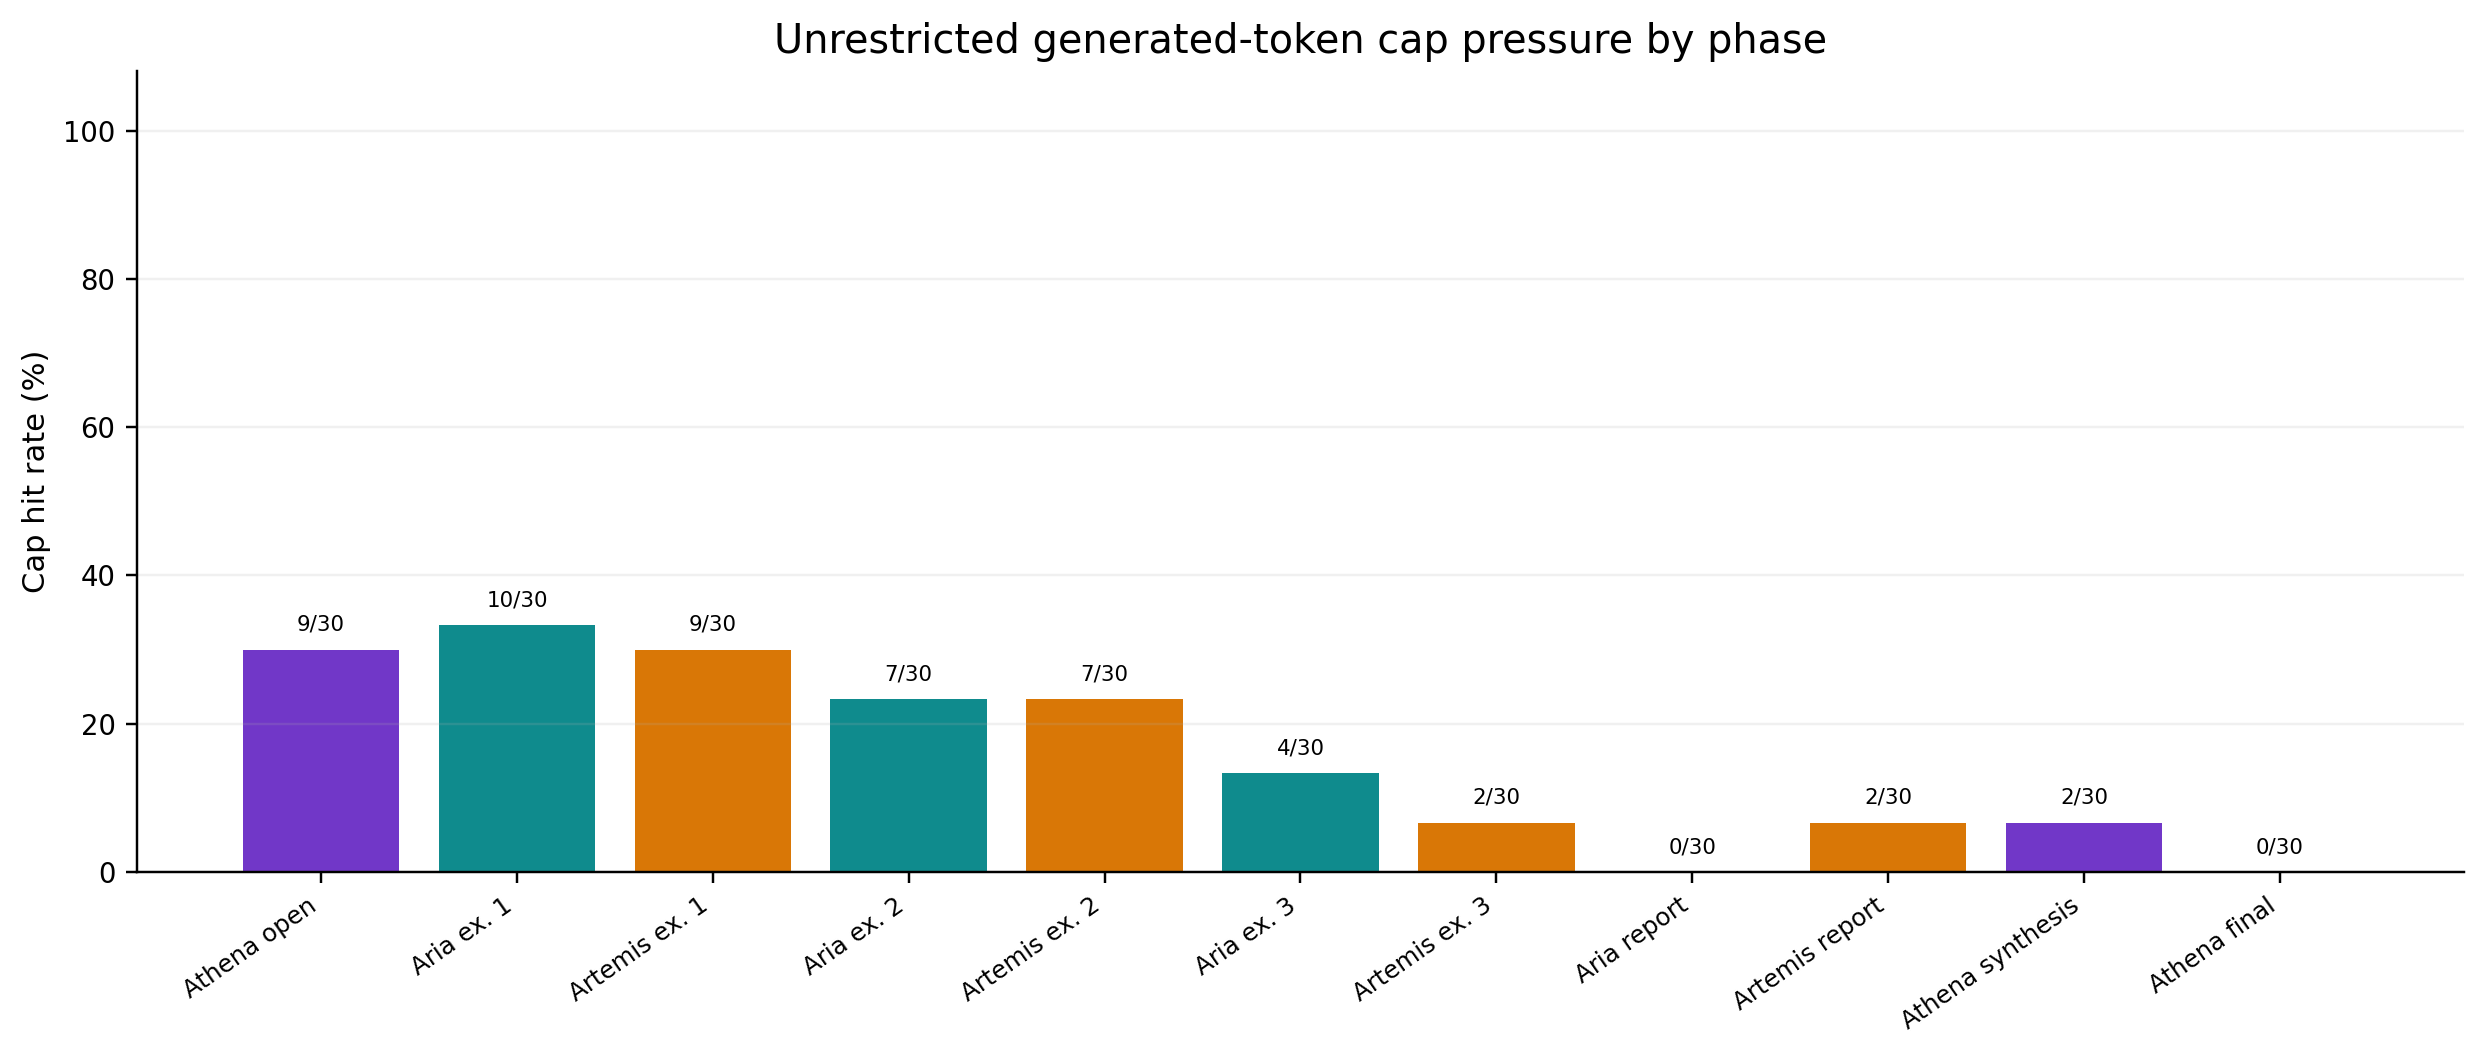
\includegraphics[width=\linewidth]{diagrams/aime2026_unrestricted_token_cap_pressure.png}
\caption{Unrestricted one-loop generated-token cap pressure by controller phase. The expanded budget reduces some cap pressure but does not eliminate saturation in long-route problems.}
\label{fig:aime2026-unrestricted-cap-pressure}
\end{figure}

\begin{figure}[H]
\centering
\begin{minipage}{0.50\linewidth}
\centering
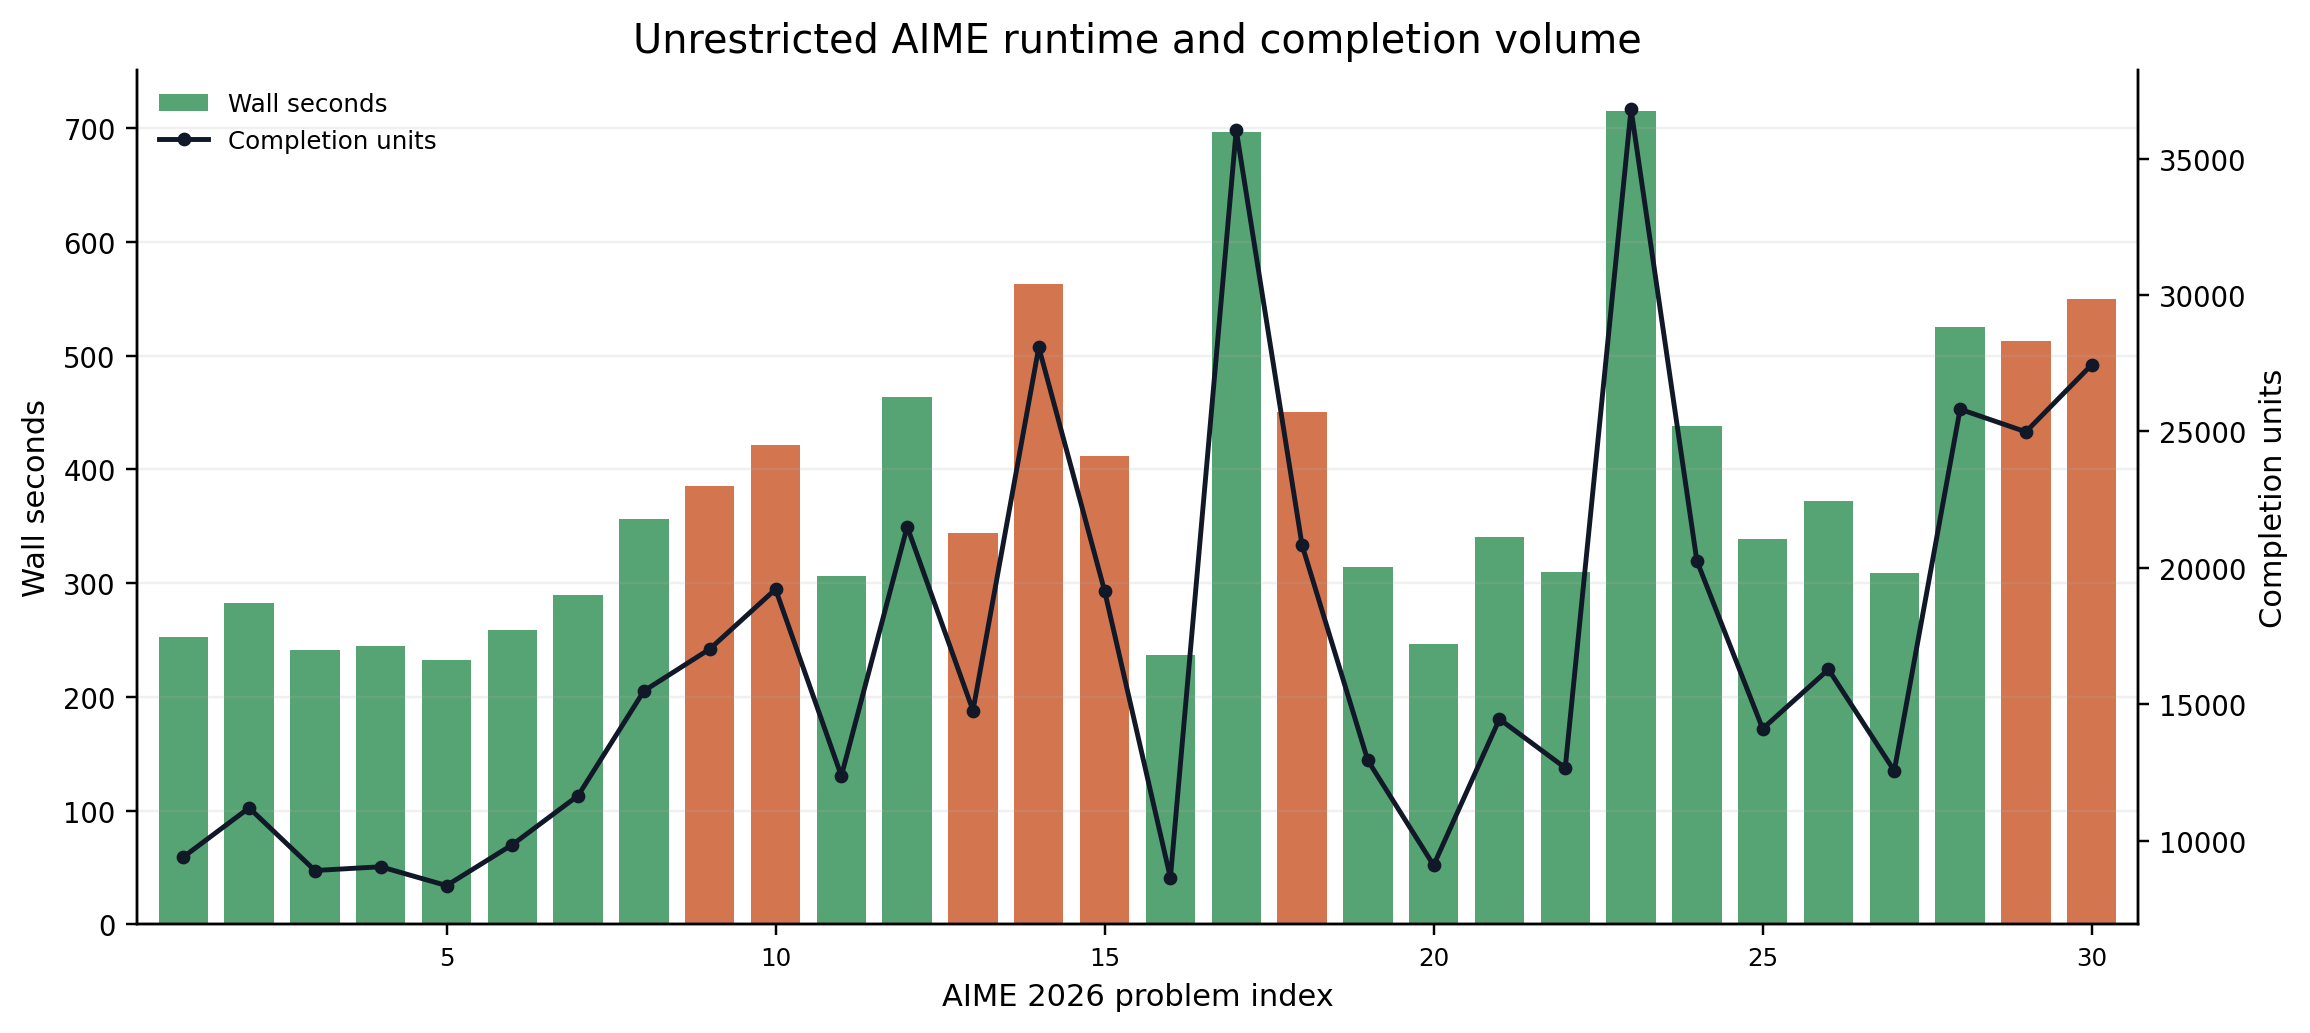
\includegraphics[width=\linewidth]{diagrams/aime2026_unrestricted_runtime_tokens.png}
\end{minipage}
\hfill
\begin{minipage}{0.46\linewidth}
\centering
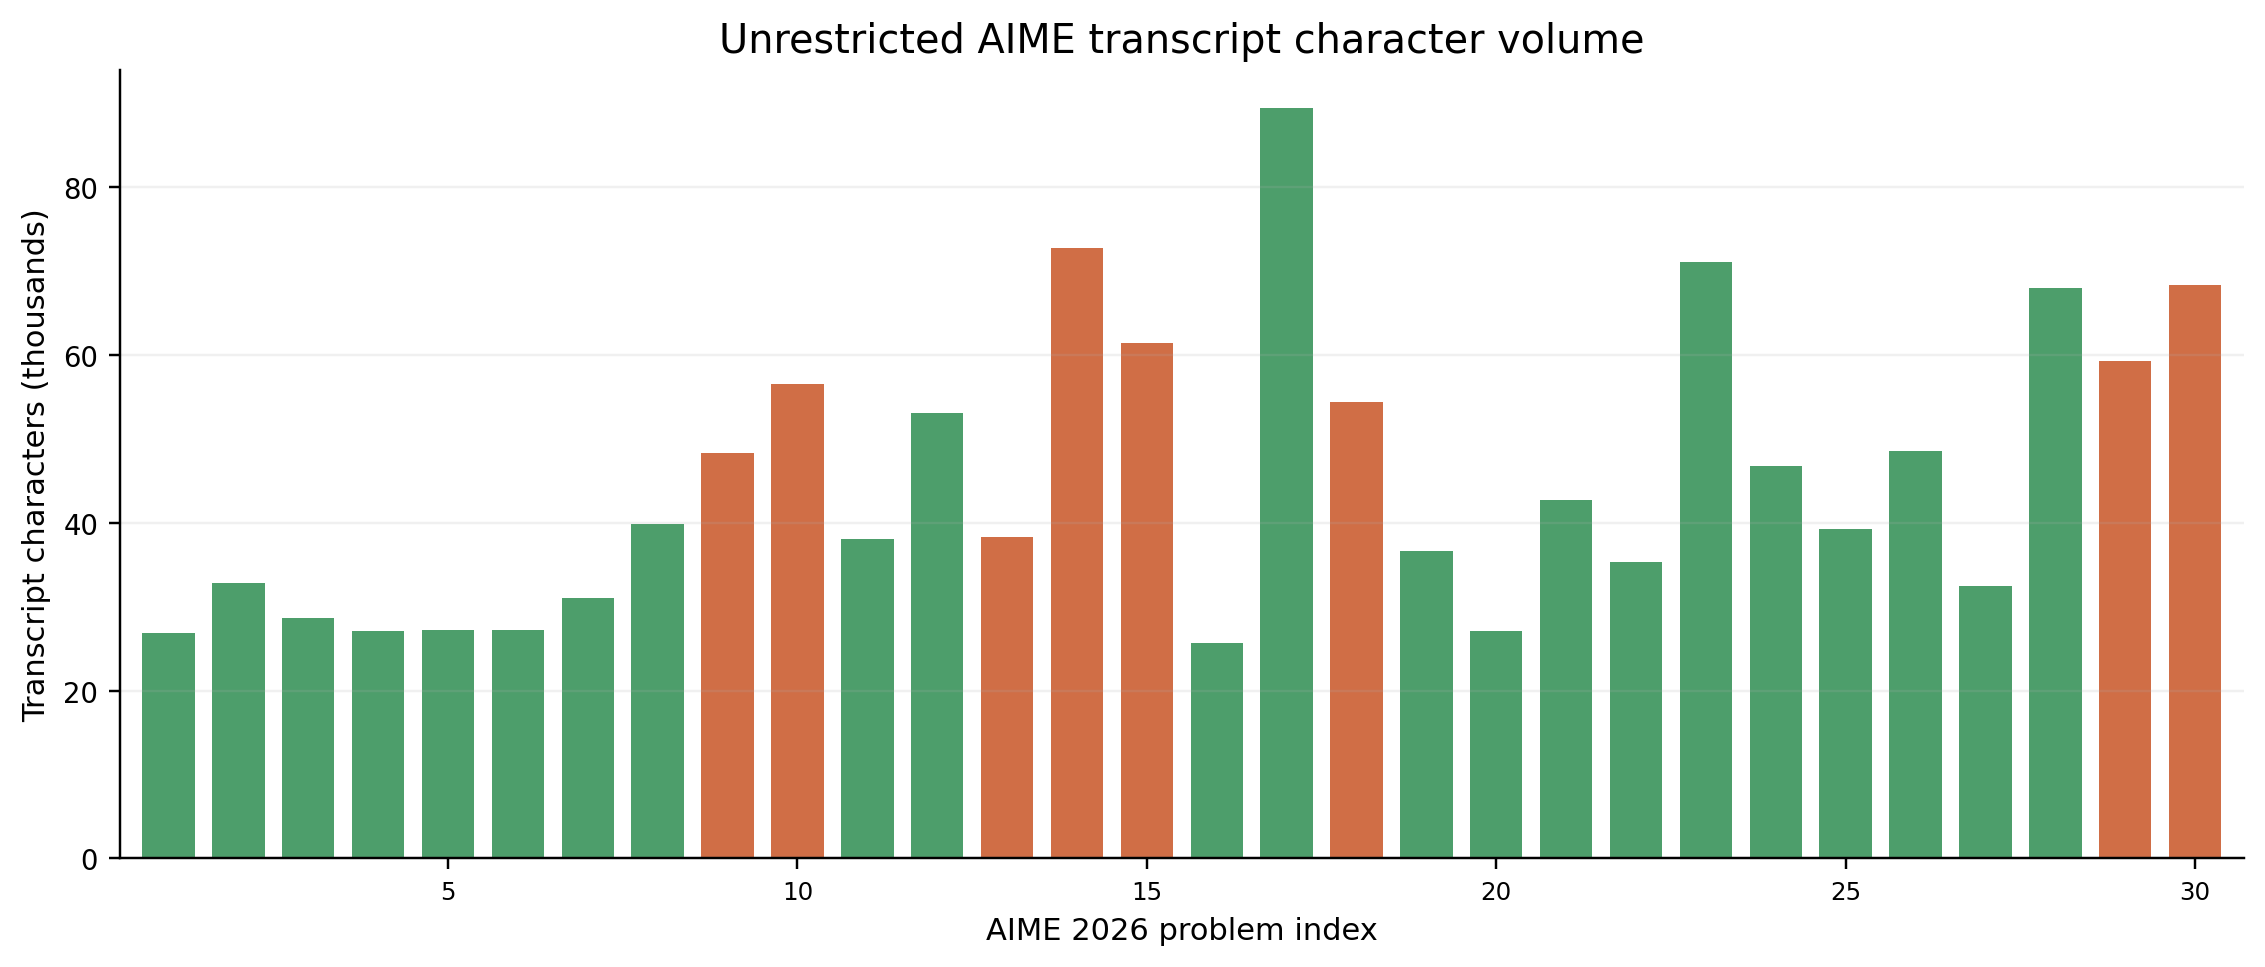
\includegraphics[width=\linewidth]{diagrams/aime2026_unrestricted_transcript_chars.png}
\end{minipage}
\caption{Unrestricted AIME runtime, completion volume, and transcript character volume. The chart records the cost of making the one-loop controller less compressed.}
\label{fig:aime2026-unrestricted-runtime-volume}
\end{figure}

\subsection{Comparison Between Frozen and Unrestricted AIME Runs}

The two AIME runs isolate a useful controller knob. The frozen run uses one loop with two peer exchanges and pruned caps; the unrestricted run keeps one loop but expands caps and adds a third peer exchange. Accuracy rises from 15/30 to 22/30. At the problem level, every frozen correct answer remains correct in the unrestricted run, seven frozen misses are recovered, and eight problems remain missed. No problem is lost by the unrestricted run.

\begin{figure}[H]
\centering
\begin{minipage}{0.46\linewidth}
\centering
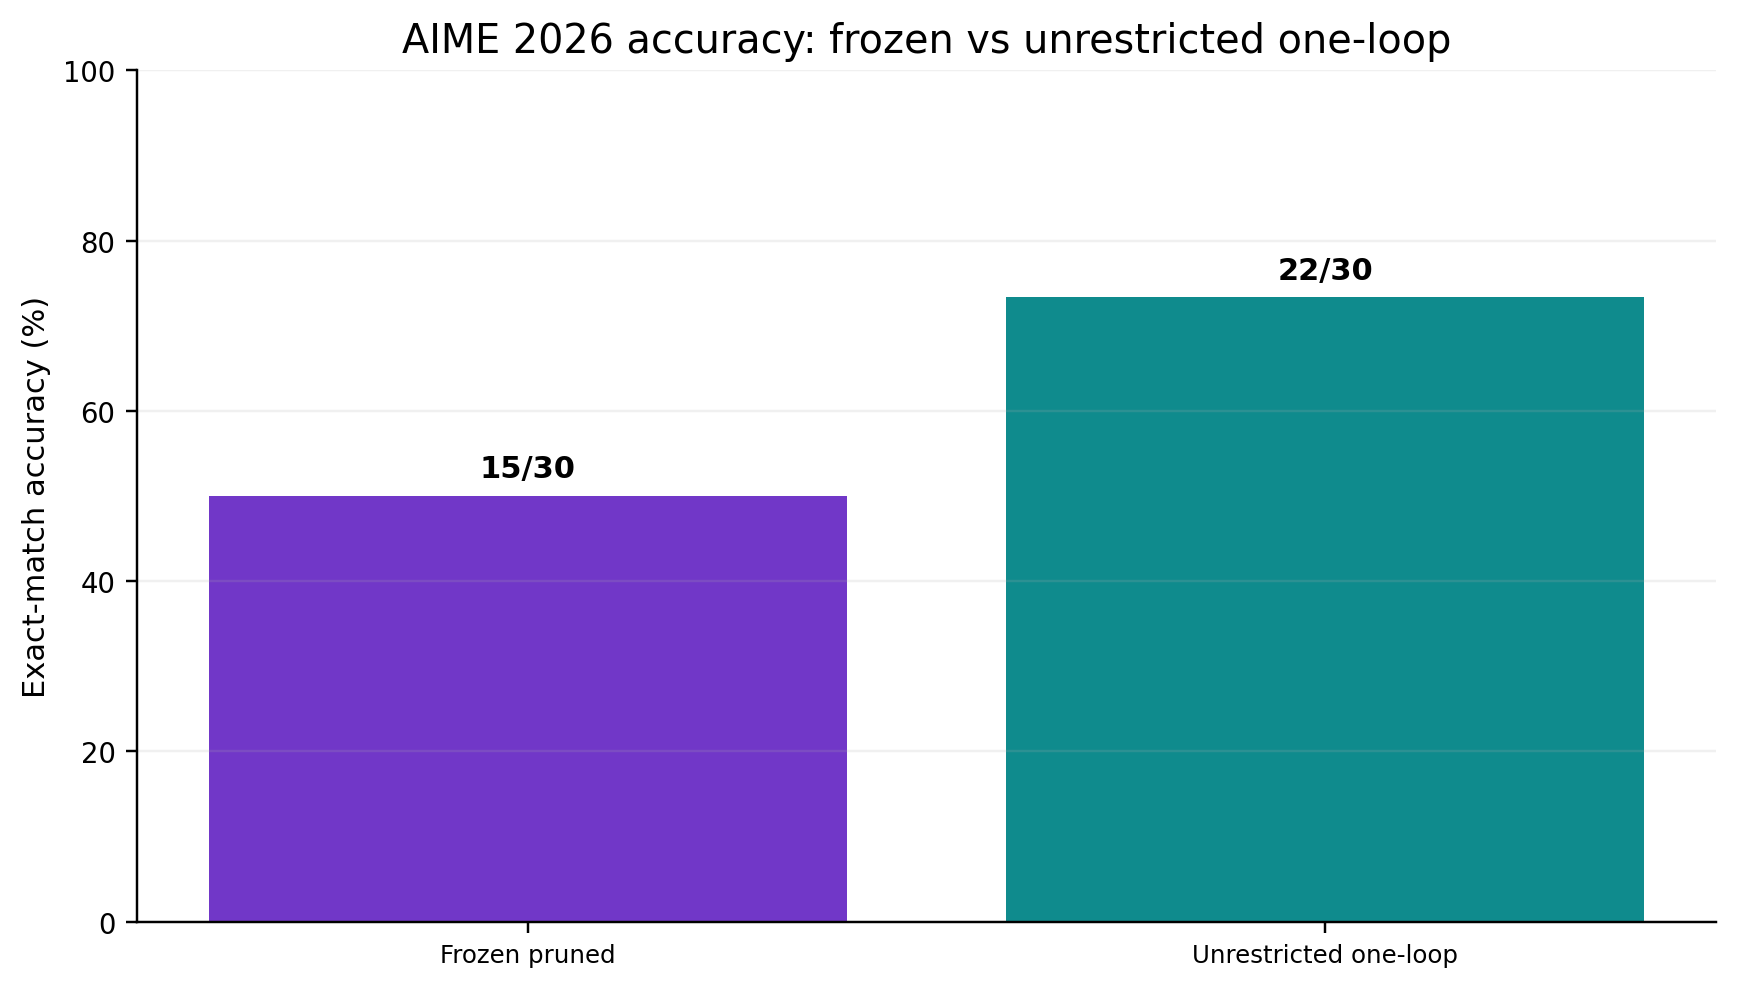
\includegraphics[width=\linewidth]{diagrams/aime2026_frozen_vs_unrestricted_accuracy.png}
\end{minipage}
\hfill
\begin{minipage}{0.50\linewidth}
\centering
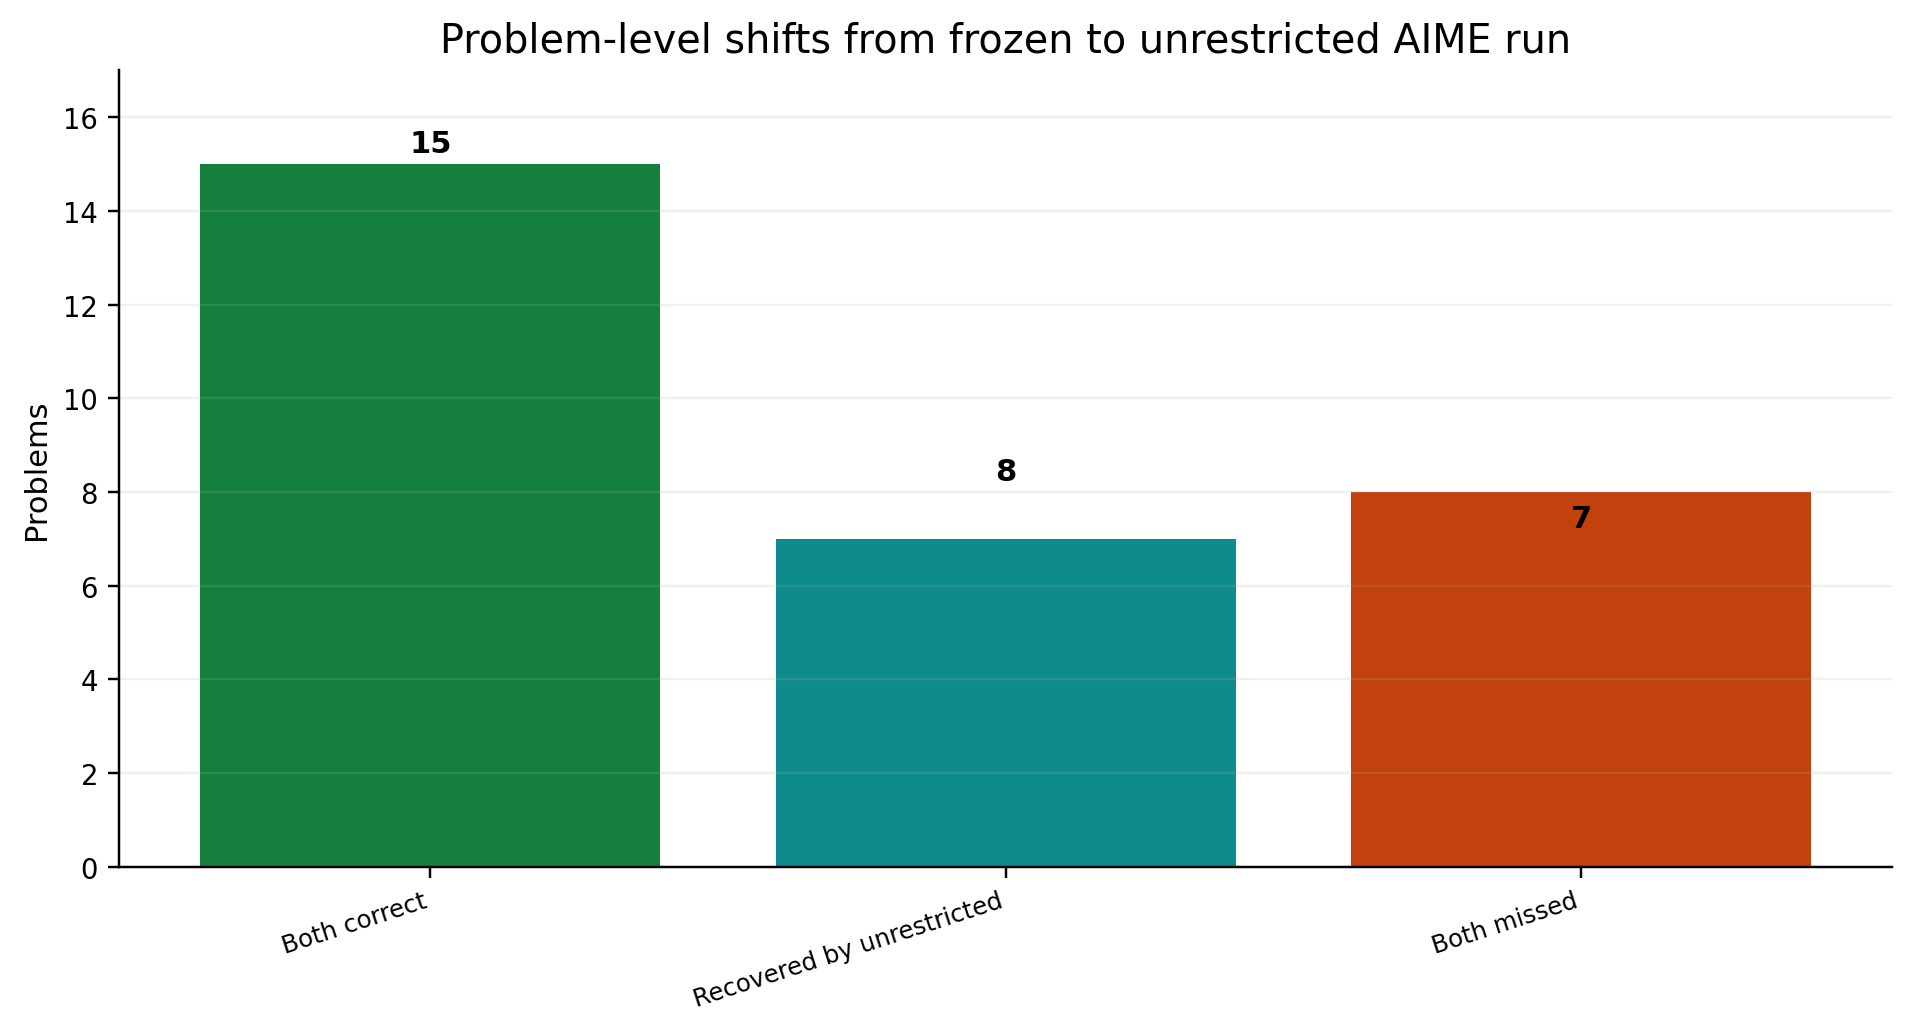
\includegraphics[width=\linewidth]{diagrams/aime2026_frozen_vs_unrestricted_problem_shifts.png}
\end{minipage}
\caption{AIME 2026 exact-match comparison. The unrestricted one-loop run improves from 15/30 to 22/30 and recovers seven frozen misses without losing any frozen correct problem.}
\label{fig:aime2026-frozen-vs-unrestricted-accuracy}
\end{figure}

The gain is concentrated where the frozen run was budget-limited. Figure~\ref{fig:aime2026-frozen-vs-unrestricted-band-closeout} shows improved middle and late bands and substantially improved majority-vote fallback calibration. The strict-consensus count remains stable, while the majority fallback becomes much more useful under the less compressed peer exchange.

\begin{figure}[H]
\centering
\begin{minipage}{0.48\linewidth}
\centering
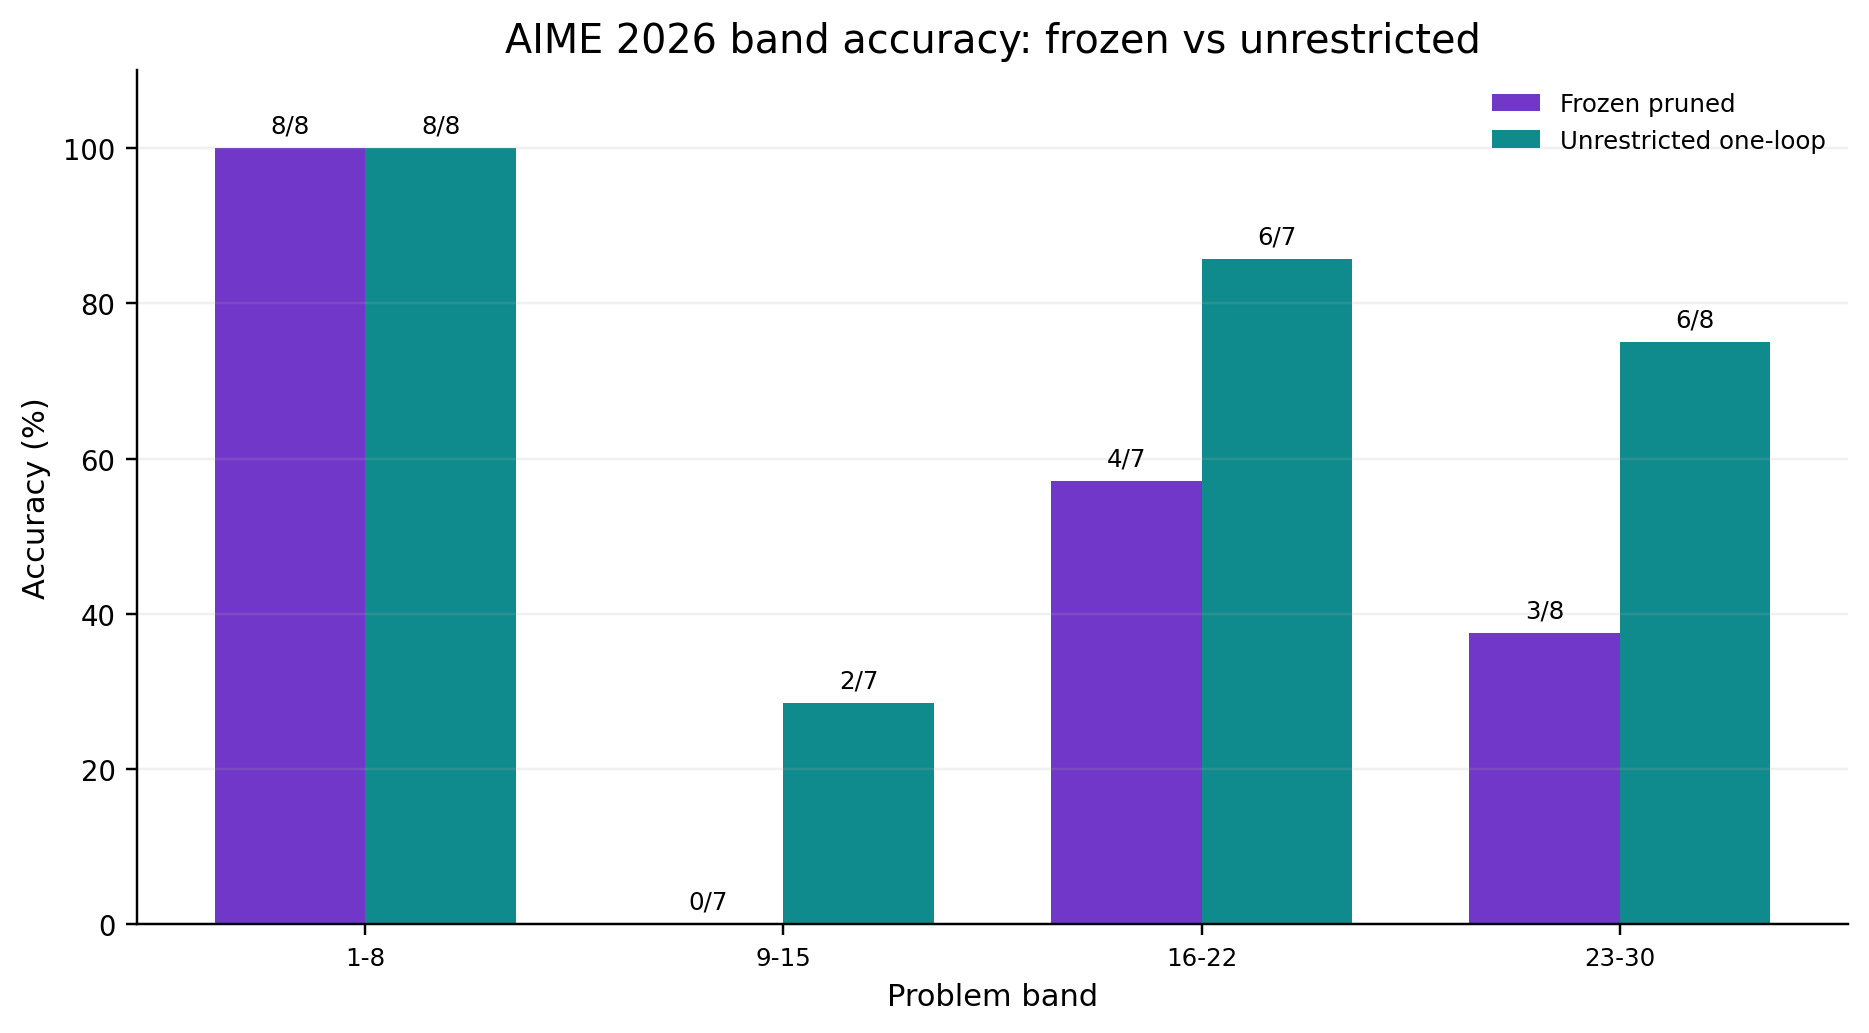
\includegraphics[width=\linewidth]{diagrams/aime2026_frozen_vs_unrestricted_band_accuracy.png}
\end{minipage}
\hfill
\begin{minipage}{0.48\linewidth}
\centering
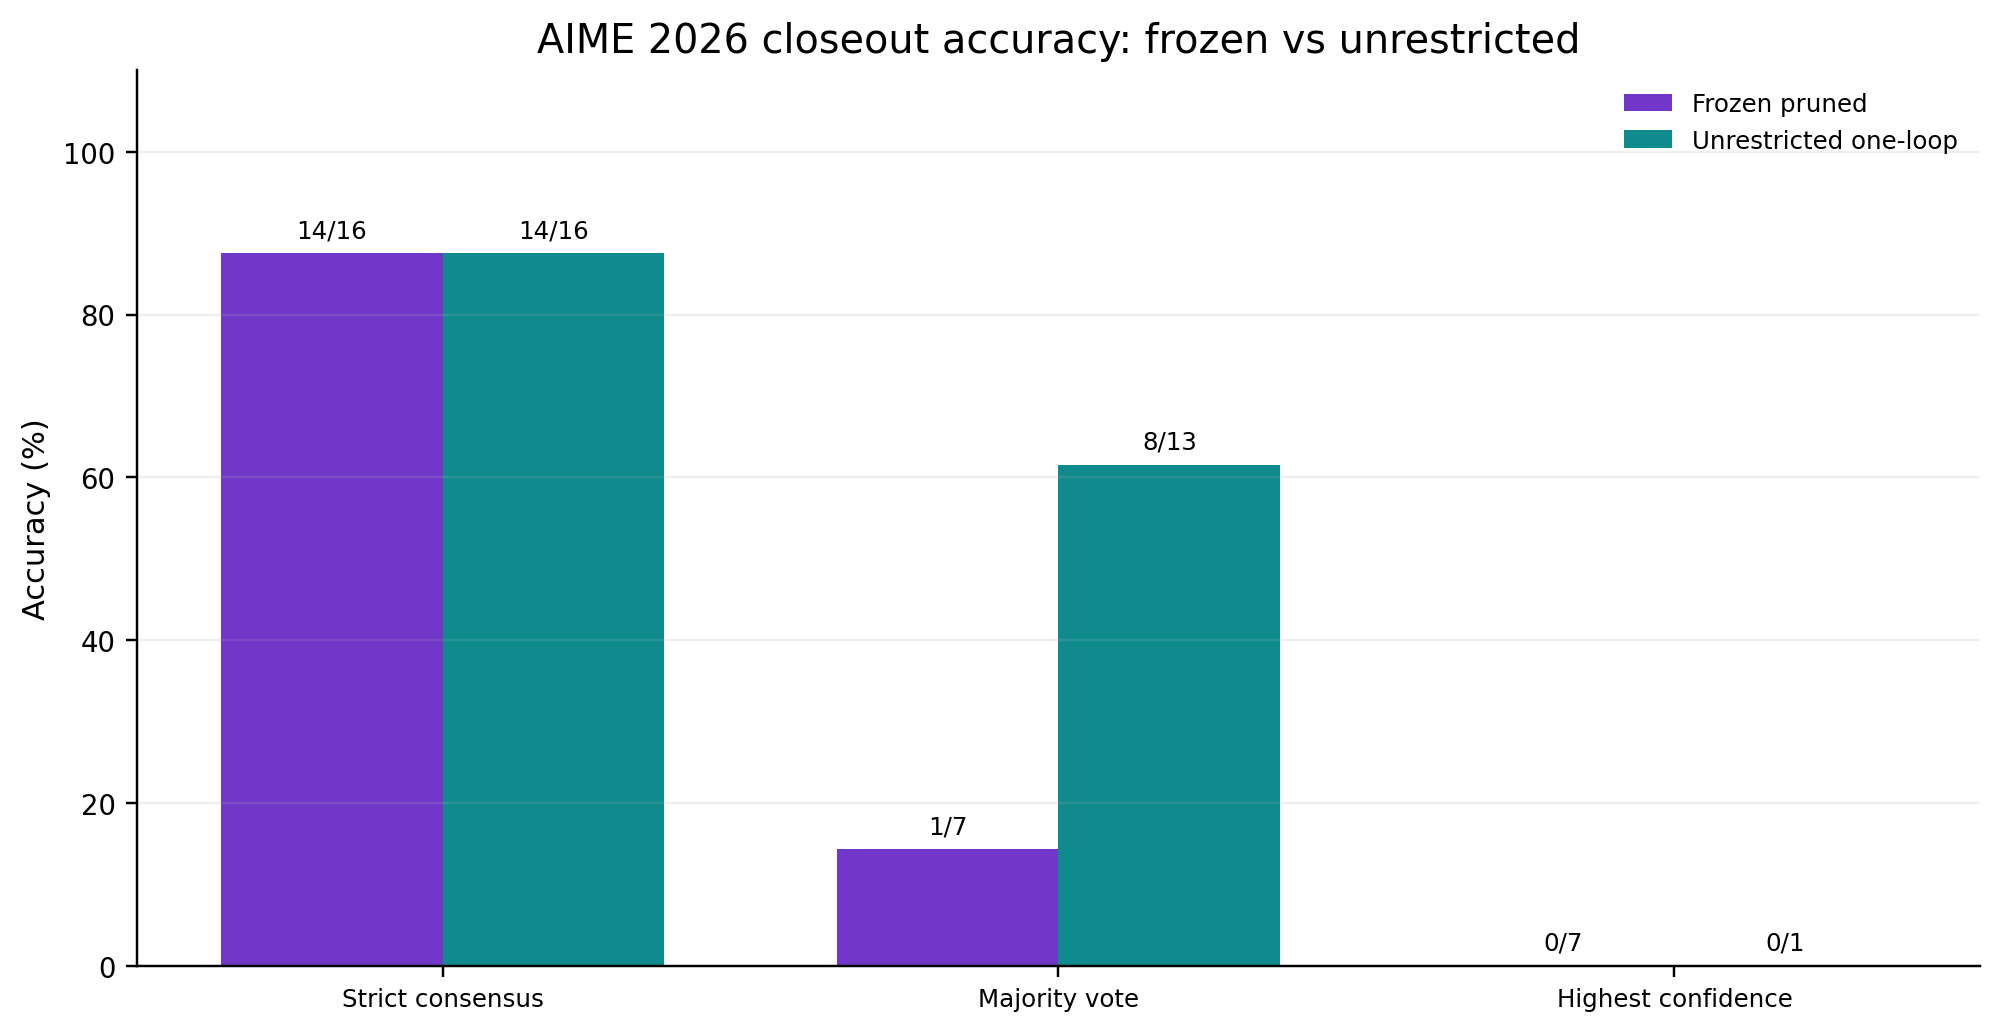
\includegraphics[width=\linewidth]{diagrams/aime2026_frozen_vs_unrestricted_closeout_accuracy.png}
\end{minipage}
\caption{Frozen versus unrestricted AIME band accuracy and closeout-mode accuracy. Expanded one-loop reasoning mainly improves the hard middle and late bands and makes majority fallback less brittle.}
\label{fig:aime2026-frozen-vs-unrestricted-band-closeout}
\end{figure}

The resource tradeoff is also explicit. The unrestricted run takes about \(2.08\times\) wall time per problem, \(2.19\times\) completion volume per problem, and \(2.30\times\) transcript character volume per problem relative to the frozen run. Figure~\ref{fig:aime2026-frozen-vs-unrestricted-resource} summarizes those multiples. Figures~\ref{fig:aime2026-frozen-vs-unrestricted-delta} then show where the extra completion and transcript volume was spent.

\begin{figure}[H]
\centering
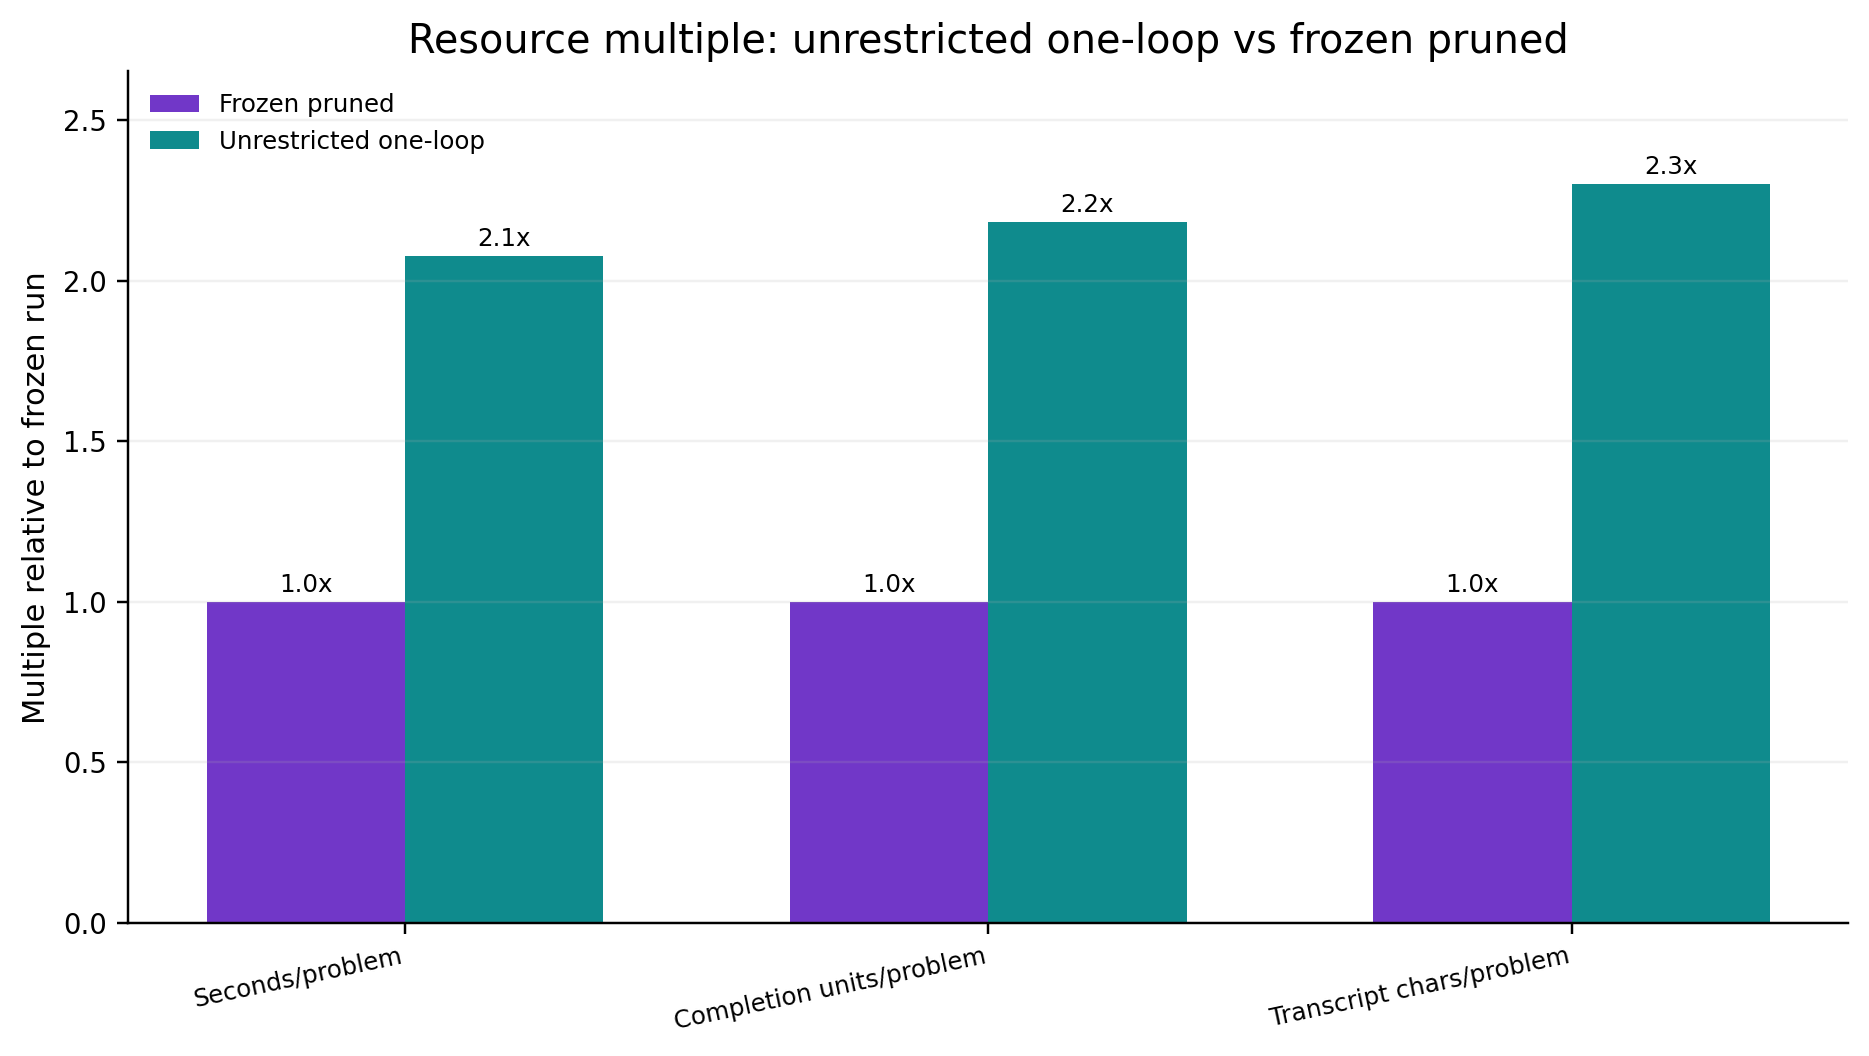
\includegraphics[width=0.82\linewidth]{diagrams/aime2026_frozen_vs_unrestricted_resource_multiple.png}
\caption{Resource multiple for unrestricted one-loop AIME relative to the frozen pruned run. The accuracy gain comes with roughly doubled wall time and generated/transcript volume.}
\label{fig:aime2026-frozen-vs-unrestricted-resource}
\end{figure}

\begin{figure}[H]
\centering
\begin{minipage}{0.50\linewidth}
\centering
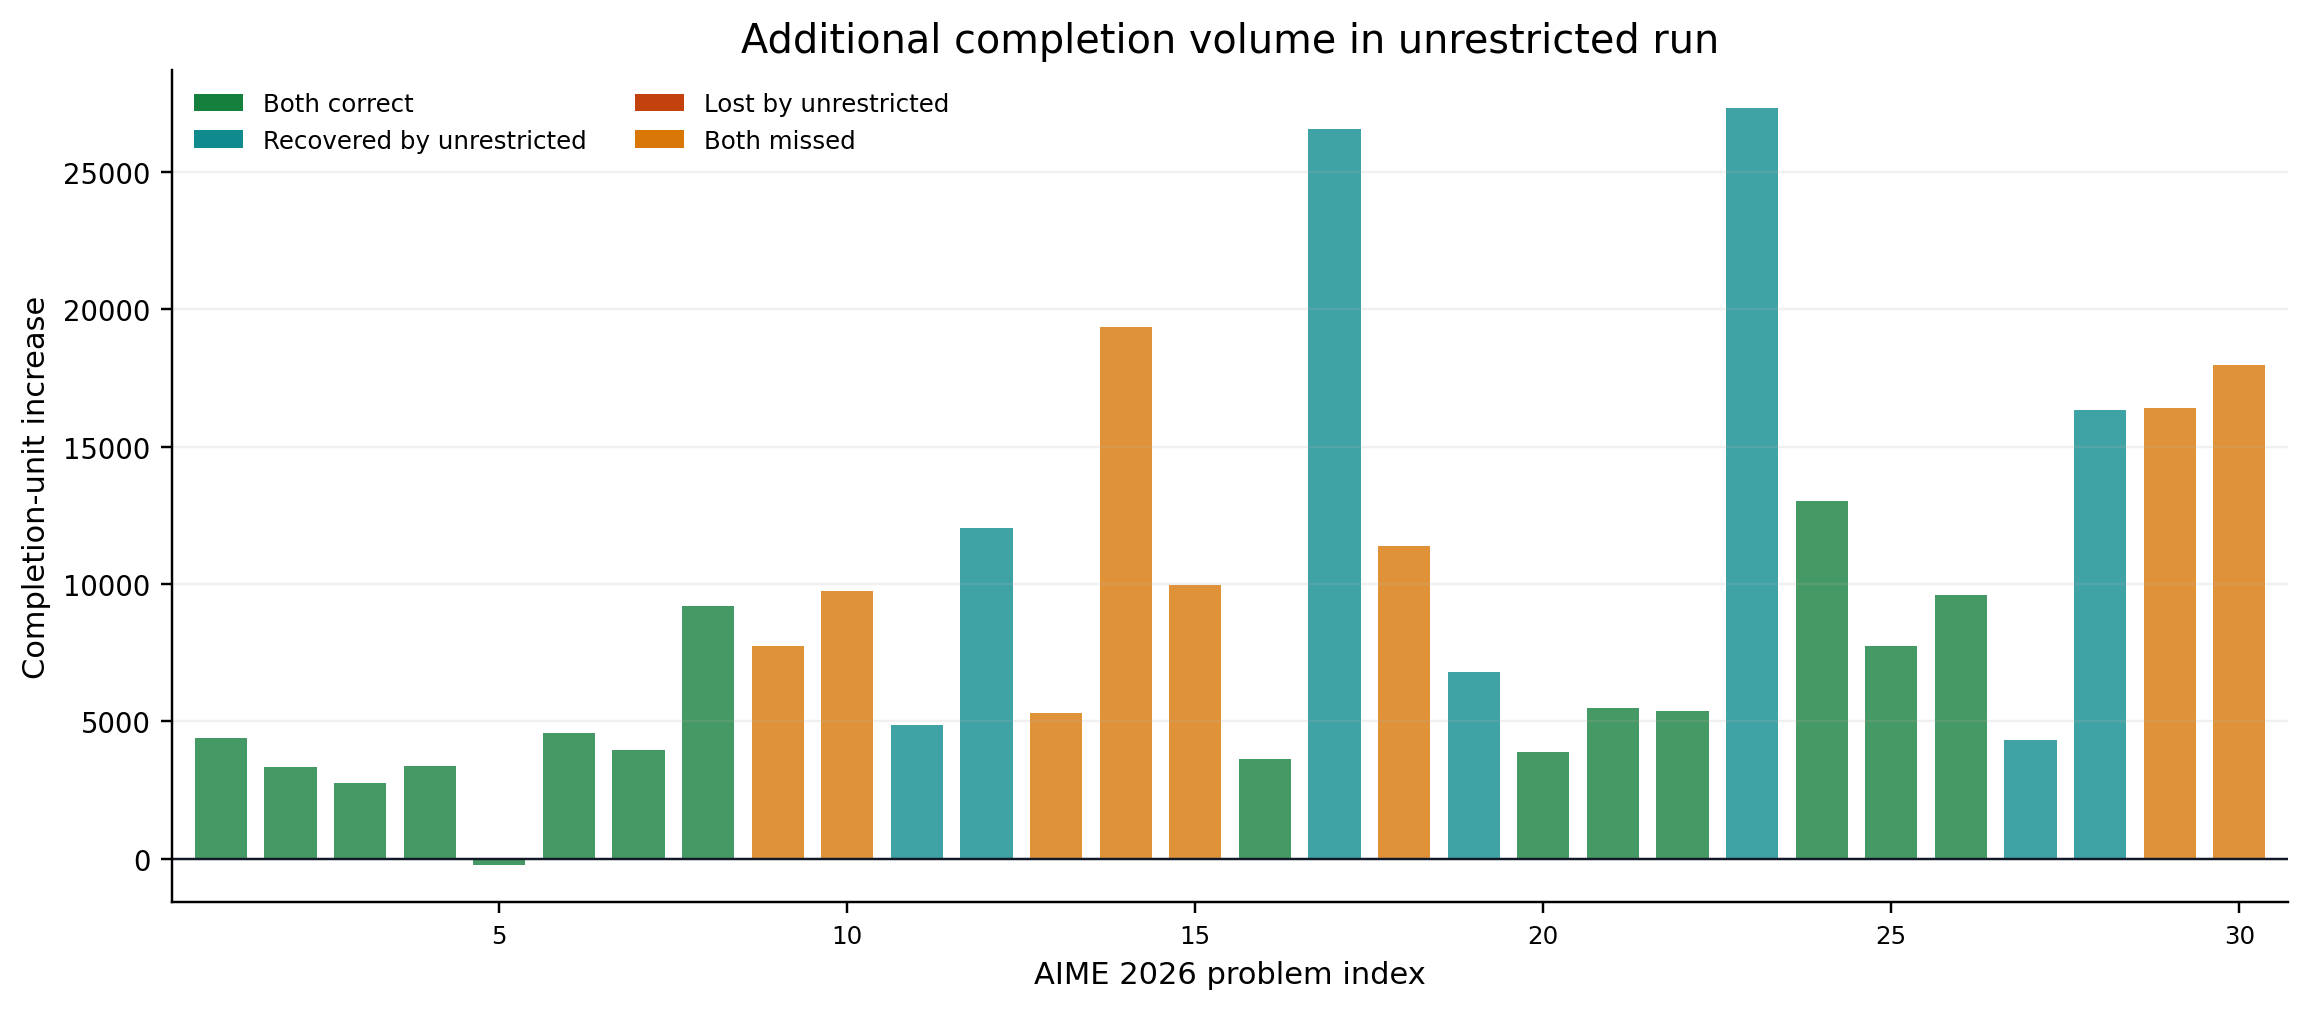
\includegraphics[width=\linewidth]{diagrams/aime2026_frozen_vs_unrestricted_completion_delta.png}
\end{minipage}
\hfill
\begin{minipage}{0.46\linewidth}
\centering
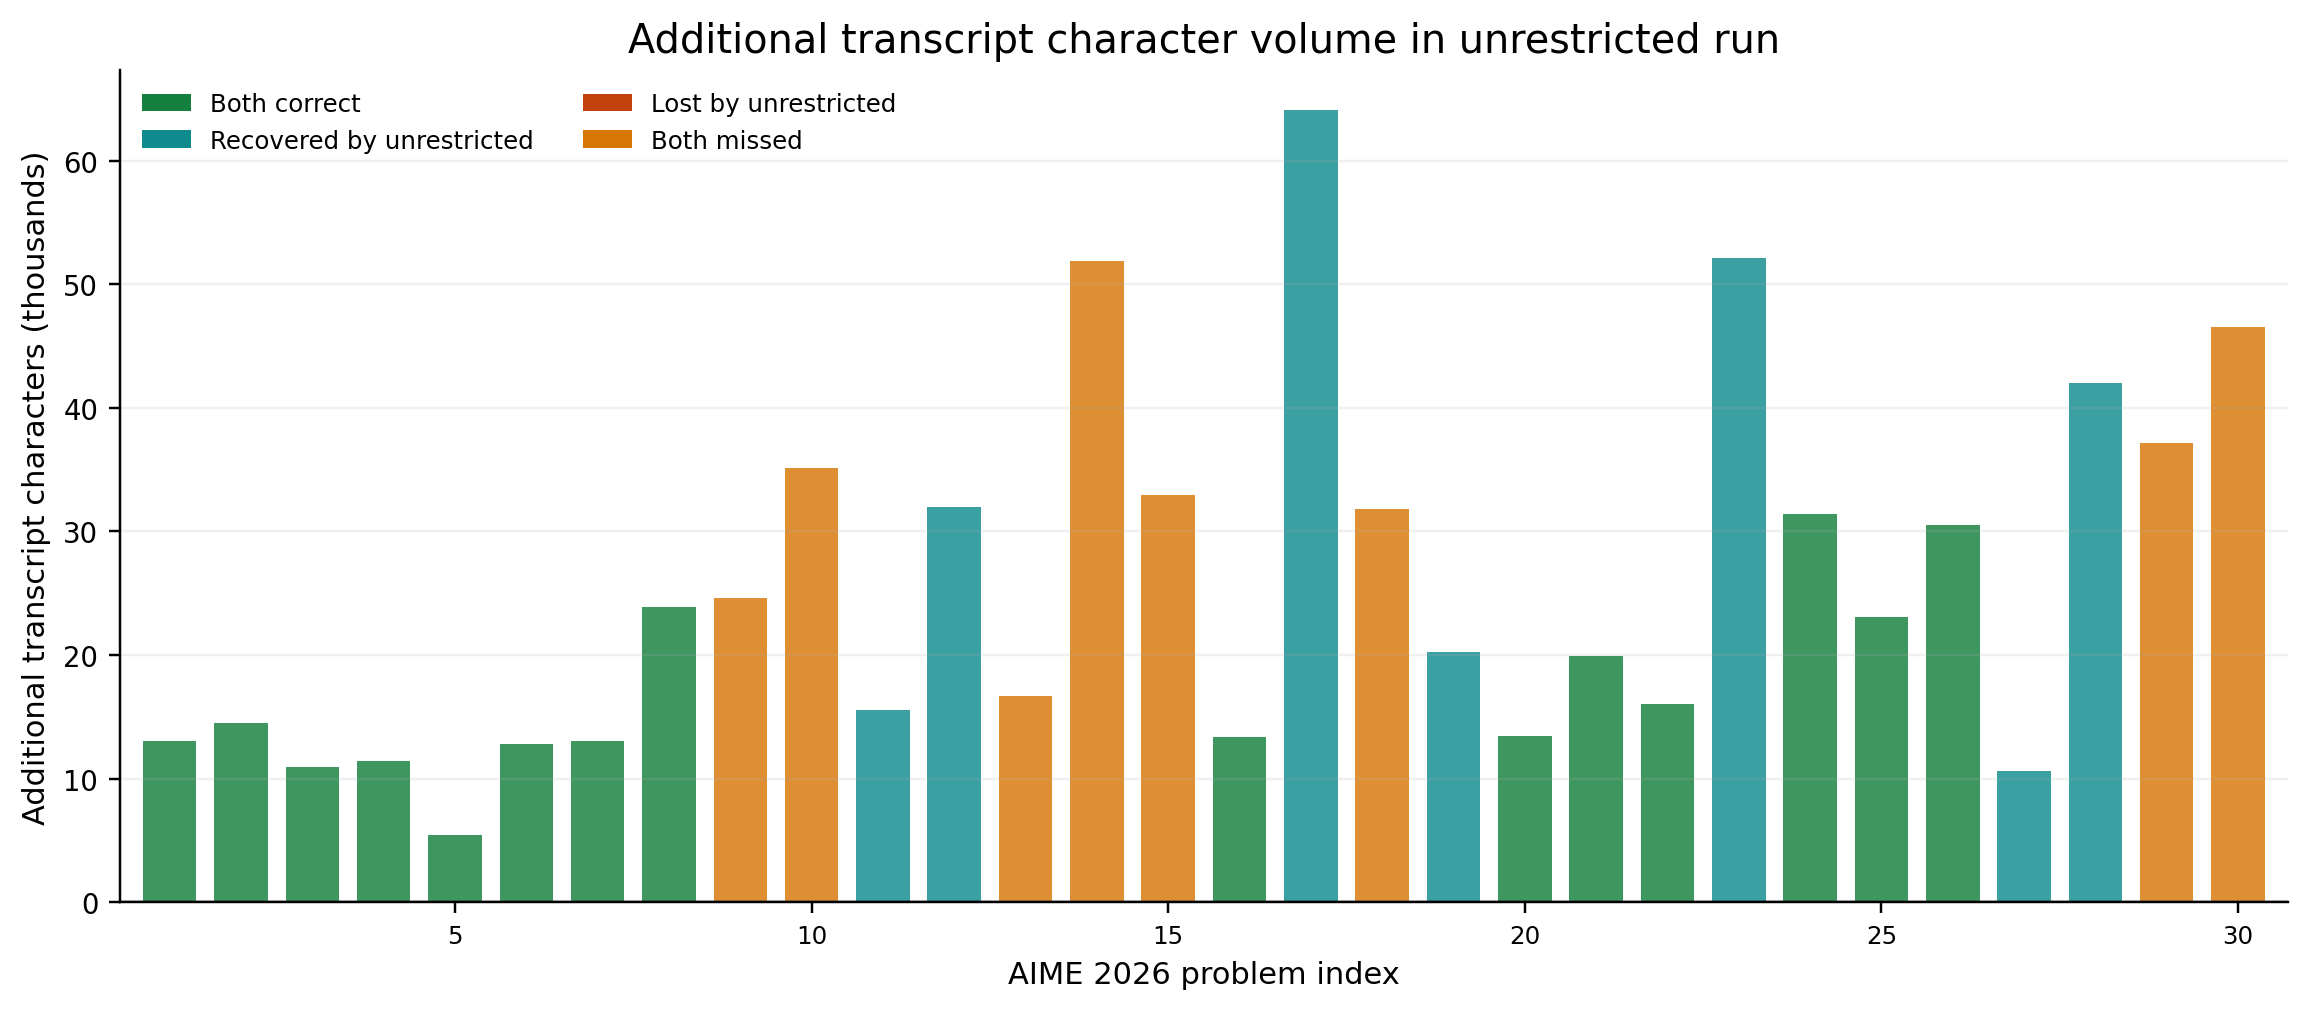
\includegraphics[width=\linewidth]{diagrams/aime2026_frozen_vs_unrestricted_transcript_delta.png}
\end{minipage}
\caption{Additional completion volume and transcript-character volume in the unrestricted AIME run. Teal bars mark problems recovered by the unrestricted setting.}
\label{fig:aime2026-frozen-vs-unrestricted-delta}
\end{figure}

The 22/30 unrestricted run is therefore an observed operating point, not an architectural ceiling. The stronger conclusion is that adding reasoning room changed the run materially while preserving the same controller algorithm and fixed model family. The next question is therefore not whether AEN has exhausted its design space, but how far the loop, exchange, and output-token budgets can be scaled before wall time, repetition, or fallback calibration become the binding constraint. Section~\ref{sec:scaling-plan} converts that question into explicit ceiling calculations and proposed sweeps.

\subsection{Proposed benchmark suite}

A larger evaluation should report, at minimum, the following:

\begin{itemize}
  \item \textbf{Mathematical accuracy}: exact-answer accuracy on held-out contest-style problems, with external, attached, or internal status stated separately.
  \item \textbf{Verification calibration}: frequency with which verified answers are correct, unverified answers are correct, and rejected answers would have been correct.
  \item \textbf{Finalization validity}: rate of schema-valid final answers, mismatch between transcript answer and emitted answer, and fallback mode distribution.
  \item \textbf{Contamination controls}: dataset provenance, boot-memory sanitization status, prompt audit status, and answer-bearing residual checks.
  \item \textbf{Resource profile}: wall time, graphics-processing-unit memory, token counts, context length, and per-role budget.
\end{itemize}

\section{Scaling Plan}
\label{sec:scaling-plan}

The AIME comparison shows that AEN has practical runtime knobs before any model weights are changed. The frozen run and the unrestricted run use the same one-loop controller family, but changing peer-exchange count and per-turn generation budgets moves exact accuracy from 15/30 to 22/30. The scaling plan should therefore combine a token-ceiling analysis with a controlled knob sweep rather than a single larger run. Each setting must preserve the same artifact trail: boot log, prompt budget, transcript, result payload, finalization mode, scoring file, and resource summary.

\subsection{Output-token ceiling analysis}

The first ceiling to quantify is the amount of model-generated reasoning text that the controller can permit. In the unrestricted AIME run, AEN used one loop, three Aria--Artemis exchange pairs, peer reports, Athena synthesis, and a short finalization turn. Let \(L\) denote the maximum loop budget and \(E\) denote the number of Aria--Artemis exchange pairs per loop. Under the recorded unrestricted caps, the configured output-token ceiling per problem is
\[
C_{\mathrm{cap}}(L,E)
=
L\bigl(4096 + 2E\cdot4096 + 2\cdot4096 + 2048\bigr) + 128.
\]
The terms correspond to Athena opening, Aria and Artemis exchange turns, Aria and Artemis reports, Athena synthesis, and the final one-line emission. This is a ceiling, not an observed consumption claim: it assumes every bounded generation turn reaches its cap.

The observed unrestricted run gives a second, data-anchored projection. Its mean Athena opening was 2876 tokens, the mean Aria--Artemis exchange pair was 3701 tokens, the two peer reports together used 2246 tokens, Athena synthesis used 735 tokens, and finalization used 12 tokens. The observed-rate projection is therefore
\[
C_{\mathrm{obs}}(L,E)
=
L\bigl(2876 + 3701E + 2246 + 735\bigr)+12.
\]
For the recorded setting \(L=1,E=3\), this reconstructs the measured unrestricted mean of approximately 16,972 completion tokens per problem. For a five-loop, ten-exchange study, the configured ceiling becomes 481,408 output tokens per problem, while the observed-rate projection is 214,366 output tokens. The latter number is not an accuracy forecast; it is a resource forecast showing that AEN can allocate a much larger reasoning trace when the runtime is allowed to focus on a hard problem. In a single-problem solve, a 214k-token observed-rate trace is comfortably below a one-million-token role-context reference. Even using the stricter configured ceiling, two such ceiling-sized hard-problem attempts occupy about 963k output tokens, leaving the scaling question as a scheduling and wall-time problem rather than an immediate context-cap impossibility.

\begin{figure}[p]
\centering
\begin{minipage}{0.49\linewidth}
\centering
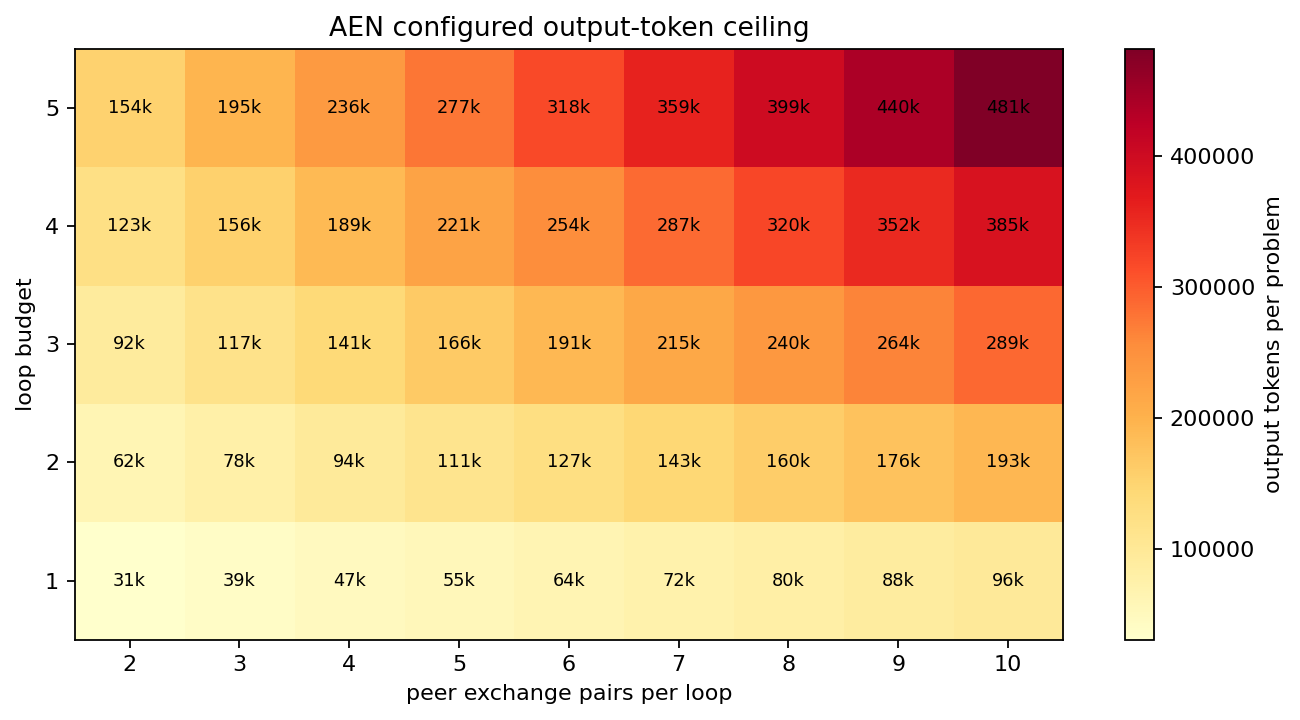
\includegraphics[width=\linewidth]{diagrams/aen_output_ceiling_heatmap.png}
\end{minipage}
\hfill
\begin{minipage}{0.49\linewidth}
\centering
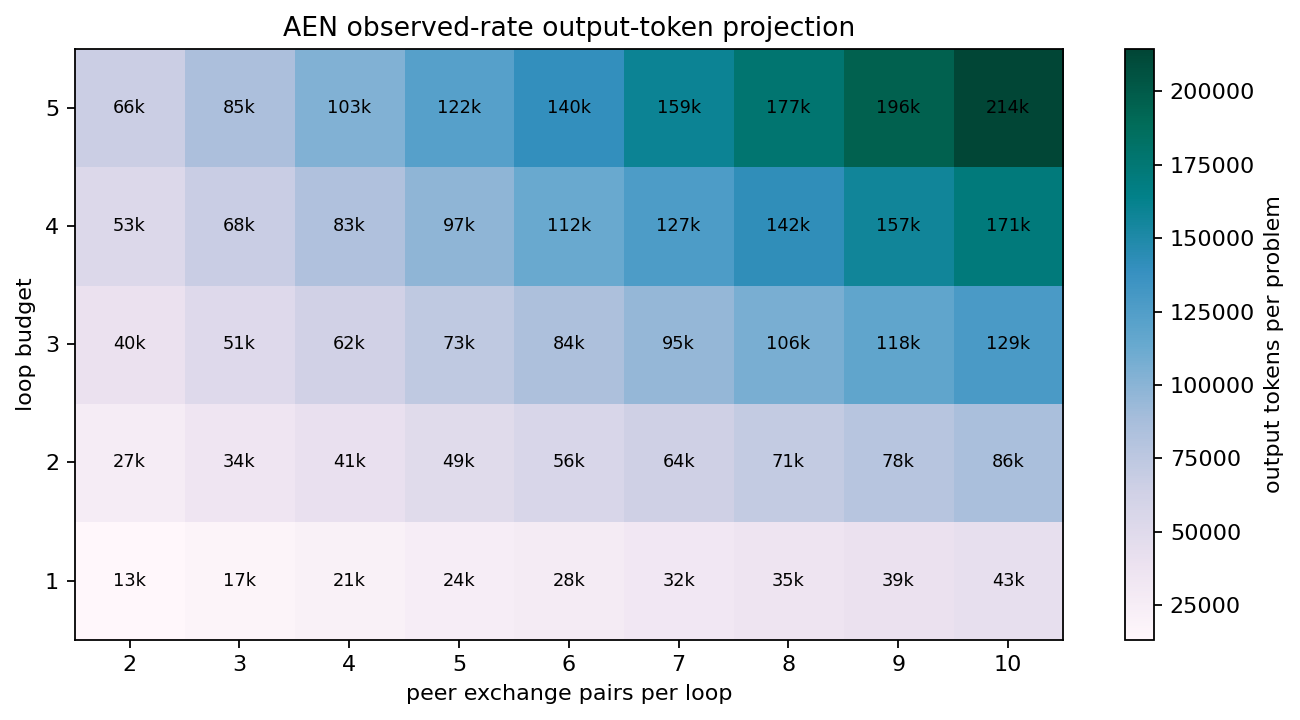
\includegraphics[width=\linewidth]{diagrams/aen_observed_projection_heatmap.png}
\end{minipage}
\caption{AEN output-token ceiling and observed-rate projection by loop budget and exchange count. The left panel is the configured cap envelope; the right panel uses the mean completion profile measured in the unrestricted AIME run. The top-right observed-rate point is the 214k-token hard-problem planning case discussed in the text.}
\label{fig:aen-output-ceiling}
\end{figure}

\begin{figure}[p]
\centering
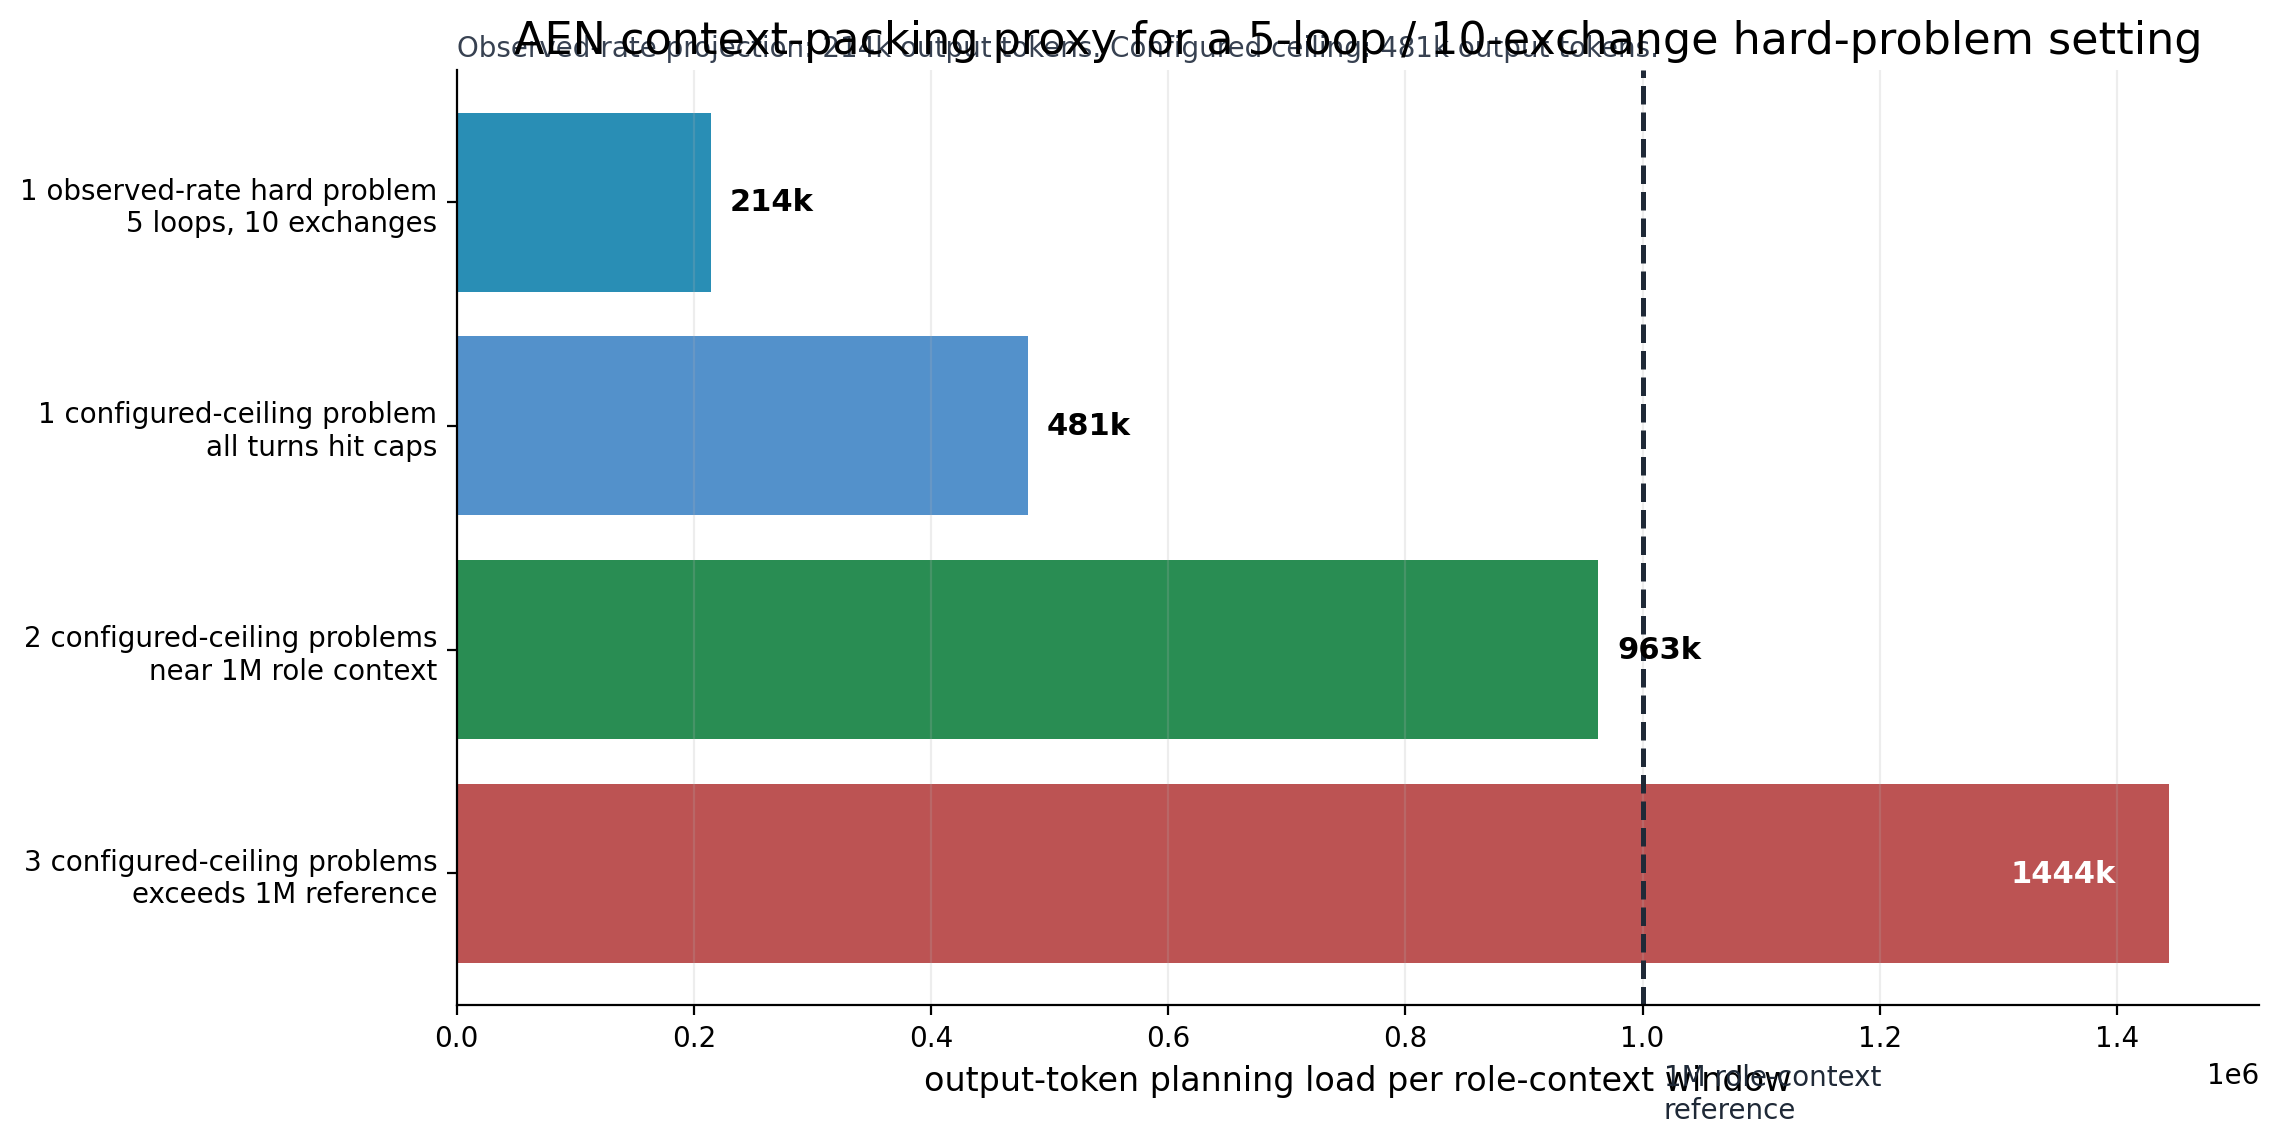
\includegraphics[width=0.92\linewidth]{diagrams/aen_context_packing_estimate.png}
\caption{Context-packing proxy for the five-loop, ten-exchange hard-problem setting. The observed-rate projection is 214k output tokens for one hard problem; the configured ceiling is 481k. Two ceiling-sized hard-problem attempts remain just under a one-million-token role-context reference, while three exceed it.}
\label{fig:aen-context-packing}
\end{figure}

This analysis explains why the unrestricted run should not be treated as a final ceiling. A Qwen-family long-context runtime gives the controller enough room to test materially larger reasoning schedules: more exchange pairs, more loops, and larger synthesis turns can be attempted without changing weights. The expected benefit is not automatic. It must come from additional proof construction, critique, self-consistency pressure, and repair opportunities rather than from token volume itself \citep{wang2022selfconsistency,madaan2023selfrefine}. The planning target is therefore an H100-class or comparable high-memory offline run that sweeps \(L\) and \(E\) while recording whether added output tokens produce new correct answers, repeated text, or merely longer incorrect routes.

\subsection{Controller knobs to scale}

The most direct knobs are the maximum loop count, peer-exchange count, per-role generation caps, synthesis budget, fallback eligibility, and memory-certification depth. A paper-scale run can set \texttt{max\_big\_loops} as high as 5, increase exchange budgets into the 2048--8192 range, and require stricter fallback evidence. The point is not to make models talk indefinitely; it is to measure how much additional reasoning room improves exact-answer accuracy before wall time and transcript volume become inefficient.

\begin{table}[t]
\centering
\small
\begin{tabularx}{\linewidth}{p{0.22\linewidth}X X}
\toprule
Runtime knob & Example sweep & Measurement \\
\midrule
Loop budget & \(L \in \{1,2,3,5\}\) & Accuracy gain, wall-time multiple, whether later loops change answers or only preserve consensus. \\
Peer exchanges & 2, 3, 4, or 5 exchange pairs & Recovery of hard problems, repetition rate, peer divergence before reports. \\
Athena opening budget & 1024, 2048, 4096, 8192 & Route completeness, first-turn cap hits, downstream peer quality. \\
Peer exchange/report budget & 1280, 2048, 4096, 8192 & Lemma construction, audit completion, repetition or echoing. \\
Athena synthesis budget & 768, 2048, 4096 & Whether synthesis closes routes before finalization. \\
Fallback eligibility & strict consensus, majority, confidence threshold, no-fallback & Verified-answer calibration and false-positive fallback rate. \\
\rab{} certification depth & line count and probe count per role & Recall reliability, boot time, and contamination risk. \\
\bottomrule
\end{tabularx}
\caption{Controller-scaling knobs for future AEN experiments. The ranges are proposed sweeps, not completed results.}
\label{tab:controller-scaling-knobs}
\end{table}

The minimum ablation set should include:

\begin{itemize}
  \item \textbf{Single-solver baseline}: \athena{} only, with the same finalization controller.
  \item \textbf{Solver plus audit}: \athena{} and \artemis{}, without \aria{}.
  \item \textbf{Solver plus alternate proof}: \athena{} and \aria{}, without \artemis{}.
  \item \textbf{Full triad}: \athena{}, \aria{}, and \artemis{} with \rab{} and controller-managed finalization.
  \item \textbf{No safe memory}: full triad with boot certification but no solve-time memory retrieval.
  \item \textbf{No boot gate}: full triad without \rab{} eligibility, included only if contamination and safety checks permit.
\end{itemize}

For each condition, the report should include accuracy, verified-answer accuracy, final-format validity, wall time, token use, prompt length, and transcript availability. If externally specified American Invitational Mathematics Examination-style test data becomes available, it should be reported separately from local attached tests. If only internal or attached datasets are used, the paper should say so plainly.

\subsection{High-compute unrestricted future work}

The output-token analysis above scales only the controller budget. A second scaling axis is model replacement. If sufficient compute, memory, and serving stability are available, the same controller algorithm can be tested with substantially larger Qwen-family role models rather than the current 9B-class configuration. A natural next experiment is a same-family high-capacity triad, for example replacing all three roles with a Qwen 122B-A10B-class checkpoint or the nearest available high-capacity Qwen-family model at evaluation time. The hypothesis is straightforward: larger role models should improve route selection, algebraic endurance, and peer critique quality while the controller continues to provide source-of-truth handling, transcript capture, role separation, and exact finalization.

The practical AIMO3 target is a fully unrestricted stress test instead of another compressed notebook diagnostic. The proposed configuration is three upgraded high-capacity Qwen-family models, \texttt{max\_big\_loops}=5, four inner Aria--Artemis exchange pairs per loop, 8192 generated tokens available to each substantive reasoning turn, and a strengthened \rab{} gate requiring 100/100 certification lines before ordinary solving begins. This is designed to test whether the AEN controller can approach a 47/50+ exact-answer target under a compute envelope closer to the architecture's intended ceiling. It is the next high-resource experiment implied by the observed movement from the frozen run to the unrestricted one-loop run.

This experiment is proposed for completion in the nearest future. If no external support is available, the expended funds will be treated as dedicated to the betterment of science, the advancement of open mathematical reasoning systems, and the long-term usefulness of auditable inference-time architecture. Scientifically, the important requirement remains unchanged: any future score must be reported with the model identifiers, loop and token budgets, hardware envelope, transcripts, scoring file, finalization modes, \rab{} certification summary, and artifact bundle needed to audit the claim.

\begin{table}[t]
\centering
\small
\begin{tabularx}{\linewidth}{p{0.23\linewidth}X}
\toprule
Report field & Minimum content \\
\midrule
Run identity & Notebook or script revision, model sources, dataset label, and timestamp. \\
Resource envelope & Graphics-processing-unit type, wall-clock budget, context/token budgets, and offline package state. \\
\rab{} state & Required roles, pass/fail status, run id, and safe-memory mode. \\
Accuracy & Exact-answer score with external/attached/internal status stated. \\
Auditability & Transcript availability, prompt audit status, finalization mode distribution. \\
Contamination control & Evidence that evaluation answers were not present in solve-time prompt memory. \\
\bottomrule
\end{tabularx}
\caption{Minimum report card for larger-resource AEN experiments.}
\label{tab:report-card}
\end{table}

\section{Limitations}

The evidence in this paper is intentionally bounded. Apart from Vault of Echoes, the paper reports one real contest-math evaluation surface: American Invitational Mathematics Examination 2026, measured under a frozen compressed notebook configuration and an unrestricted one-loop configuration. Those two runs are valuable because they compare the same problem surface under different controller budgets, but they do not yet constitute a broad benchmark suite, a private AIMO3 result, or a final AEN ceiling.

Vault of Echoes serves a different purpose. The fresh no-answer-memory run measures how the architecture behaves when it must reason from the puzzle statements and role discipline alone. The memory-loaded 25/25 run demonstrates that Runtime-at-Boot can place canonical solution material into active context and that the controller can recover and emit the correct answers from certified context recall. It should therefore be read as a successful recall and controller-finalization test, not as evidence that the system solved all 25 Vault of Echoes problems by pure reasoning.

The remaining limitations follow directly from that evidence boundary:

\begin{itemize}
  \item The AIME evidence is a single 30-problem contest-math surface, not a multi-benchmark evaluation.
  \item The unrestricted AIME run uses one loop; the five-loop and 8192-token settings are proposed scaling tests, not completed results.
  \item The output-token ceiling analysis estimates available generation room and wall-time pressure; it does not predict accuracy by itself.
  \item Runtime-at-Boot certification demonstrates active context recall of role memory and certified lines; it is not a standalone proof of mathematical intelligence.
  \item The 25/25 Vault of Echoes memory-loaded result depends on certified context recall of known canonical solutions and must not be collapsed into the no-answer-memory reasoning result.
  \item The proposed high-capacity Qwen-family replacement path remains a planned experiment until the model identifiers, hardware envelope, transcripts, scoring file, and artifact bundle are available.
\end{itemize}

The central claim is therefore precise: AEN makes mathematical reasoning an auditable runtime process by combining certified boot memory, role-separated critique, controller-owned finalization, and explicit token-budget control. This paper contributes one test dataset surface, three role-specific training datasets, three certification-pair surfaces for the training datasets, the Canon v2.1 YAML schema for machine-readable mathematical distillation, the Runtime-at-Boot certification procedure, the three-body controller algorithm, and the artifact discipline needed to audit exact-answer runs. The present results show that changing runtime budget and context availability can materially change exact-answer behavior without changing weights. The next scientific step is to test the same controller under larger models, larger loop budgets, 100/100 boot certification, and larger generation ceilings while preserving the same evidence trail.

\bibliographystyle{plainnat}
\bibliography{references}

\end{document}
